% ---- ETD Document Class and Useful Packages ---- %
\documentclass{ucetd}
%\usepackage{oneinchmargins}
\usepackage{times}
\usepackage{relsize}
\usepackage{enumerate}
\usepackage{graphicx}
\usepackage{url}
%\usepackage{color}
\usepackage[usenames,dvipsnames]{xcolor}
%\usepackage[pagebackref]{hyperref}
%\usepackage[bookmarks=false]{hyperref}

%\hypersetup{colorlinks=true,citecolor=OliveGreen,linkcolor=Maroon,urlcolor=NavyBlue}

%\hypersetup{colorlinks=true,
%citecolor=Maroon,
%linkcolor=Green,
%urlcolor=Maroon}

%\usepackage{breakurl}
\usepackage{setspace}
\usepackage{rotating}

\usepackage{floatflt}
\usepackage{wrapfig}
\usepackage{alltt}
\usepackage{epstopdf}
\usepackage{subfigure}

%\usepackage{listings}
%\usepackage{algorithm}
%\usepackage{algorithmic}

\usepackage{fancyvrb}
%\usepackage{ulem} % for strike out,  
% \em and \sout are now strikes, use \it for italic
% never do this because now all 
\renewcommand{\ttdefault}{cmtt}

%\usepackage{colortbl} % for table color
%\usepackage{pstricks} % for gray hline
%\input{colortab} % for gray hline (must include pstricks)
%\usepackage{array}



% make sure url bib break point does not
% give undefull hbox message and the break line 
% is really nice now
\usepackage{etoolbox}
\apptocmd{\thebibliography}{\raggedright}{}{}


% -----------------------------------------------------
\usepackage{rotating}

\usepackage{subfigure,epsfig,amsfonts}
\usepackage{natbib}
\usepackage{amsmath}
\usepackage{amssymb}
\usepackage{amsthm}


% ---------------------------------------------
% name abbrvs .. 
% ---------------------------------------------
\newcommand{\infokernel}{\mbox{infokernel}}
\newcommand{\unix}{{\sc Unix}}
\newcommand{\dare}{DARE}
\def \samc {\textsc{SamC}}
\def \sampro {\textsc{SamPro}}
\def \samzoo {\textsc{SamZoo}}
\def \sammr {\textsc{SamMr}}
\def \sammace {\textsc{SamMace}}
\def \samcass {\textsc{SamCass}}
\def \sameiger {\textsc{SamEiger}}
\def \modist {\textsc{Modist}}
\def \macemc {\textsc{MaceMC}}
\def \setsudo {\textsc{Setsudo}}
\def \prefail {\textsc{PreFail}}

\def \fate {\textsc{Fate}}
\def \late {\textsc{Late}}
\def \lights {\textsc{LigHTS}}

\def \phi {$\Phi$\xspace}

\def \taxdc {TaxDC}
\def \tdc {TaxDC}
\def \sck {\textsc{SCk}\xspace}
\def \cdb {\textsc{CbsDB}}
\def \cbs {CBS}

\def \prx {\textsc{PilRx}\xspace}

\newcommand{\ts}[1]{{\tt{\small#1}}}


\def \uuu {\textbf{\textcolor{Maroon}{\textbf{$\uparrow$}}}}
\def \uu {\textbf{\textcolor{Maroon}{\textbf{$\Uparrow$}}}}
% \def \nu {\textbf{\textcolor{Maroon}{\textbf{$\nearrow$}}}} % submission only

\def \sleep {\ts{sleep()}}

\newcommand{\num}[1]{\textcolor{red}{\textbf{#1}}}
\def \numOldDeepBugs {12} 
\def \numZkDeepBugs {7}   
\def \numMrDeepBugs {3}
\def \numCsDeepBugs {2}
\def \numZkNewBugs {1}
\def \numMrNewBugs {1}
\def \numNewBugs {2}
\def \numVersions {10}
\def \numLinesSamPro {10,886}
\def \numProtocols {7}
\def \numLinesRule {35}  
\def \numMaxBugSpeedUp {271x}  
\def \numAvgBugSpeedUp {33x}    
\def \numAvgExecTime {40}

\def \numMinRedRatio {37x}  
\def \numMaxRedRatio {166x}  
\def \numRedRatioExecs {3000}

%\newcommand{\mrb}[1]{MR-#1}
%\newcommand{\zkb}[1]{ZK-#1}
%\newcommand{\zk}[1]{ZooKeeper-#1}
%\newcommand{\mr}[1]{MapReduce-#1}
%\newcommand{\cs}[1]{Cassandra-#1}

\newcommand{\jira}[3]{\href{http://issues.apache.org/jira/browse/#1-#3}{#2-#3}}

\newcommand{\mrb}[1]{\jira{MAPREDUCE}{MR}{#1}}
\newcommand{\zkb}[1]{\jira{ZOOKEEPER}{ZK}{#1}}
\newcommand{\cab}[1]{\jira{CASSANDRA}{CA}{#1}}
\newcommand{\hbb}[1]{\jira{HBASE}{HB}{#1}}
\newcommand{\hdb}[1]{\jira{HDFS}{HD}{#1}}
\newcommand{\zk}[1]{\jira{ZOOKEEPER}{ZK}{#1}}
\newcommand{\mr}[1]{\jira{MAPREDUCE}{MR}{#1}}
\newcommand{\ca}[1]{\jira{CASSANDRA}{CA}{#1}}
\newcommand{\hb}[1]{\jira{HBASE}{HB}{#1}}
\newcommand{\hd}[1]{\jira{HDFS}{HD}{#1}}


\def \ll {\ts{L}}
\def \ff {\ts{F}}
\def \pri {\ts{pr}$_{i}$}
\def \prone {\ts{pr}$_{1}$}
\def \prtwo {\ts{pr}$_{2}$}
\def \prtri {\ts{pr}$_{3}$}

\def \ls {\ts{ls}}
\def \als {\ts{als}}
\def \rals {\ts{rals}}
\def \ralsi {\ts{rals}$_{i}$}
\def \ralsone {\ts{rals}$_{1}$}
\def \ralstwo {\ts{rals}$_{2}$}
\def \ralstri {\ts{rals}$_{3}$}
\def \rags {\ts{rags}}


\def \gs {\ts{gs}}
\def \ags {\ts{ags}}
\def \nn {\ts{N}}
\def \none {\ts{N1}}
\def \ntwo {\ts{N2}}
\def \ntri {\ts{N3}}
\def \nfour {\ts{N4}}
\def \mone {\ts{m}$_{1}$}
\def \mn {\ts{m}$_{n}$}
\def \mm {\ts{m}}
\def \fone {\ts{F1}}
\def \ftwo {\ts{F2}}
\def \ftri {\ts{F3}}
\def \ma {\ts{a}}
\def \mb {\ts{b}}
\def \mc {\ts{c}}
\def \md {\ts{d}}
\def \mx {\ts{m1}}
\def \my {\ts{m2}}
\def \xx {\ts{X}}
\def \pg {\ts{pg}}
\def \pl {\ts{pl}}
\def \pp {\ts{p}}
\def \pd {\ts{pd}}
\def \pi {\ts{pi}}
\def \pm {\ts{pm}}
\def \pc {\ts{pc}}

% ---------------------------------------------
% spaces
% ---------------------------------------------
\newcommand{\vtwenty}{\vspace{20pt}}
\newcommand{\vfifteen}{\vspace{15pt}}
\newcommand{\vten}{\vspace{10pt}}
\newcommand{\vfive}{\vspace{5pt}}
\newcommand{\vthree}{\vspace{3pt}}

\newcommand{\vmintwo}{\vspace{-2pt}}
\newcommand{\vminthree}{\vspace{-3pt}}
\newcommand{\vminfive}{\vspace{-5pt}}
\newcommand{\vminten}{\vspace{-10pt}}
\newcommand{\vminfifteen}{\vspace{-15pt}}
\newcommand{\vmintwenty}{\vspace{-20pt}}

% ---------------------------------------------
% overloaded commands
% ---------------------------------------------
\newcommand{\ub}[1]{\underline{{\bf #1}}}
\newcommand{\bquote}{\vspace{-0.25cm} \begin{quote}}
\newcommand{\equote}{\end{quote}\vspace{-0.2cm} }
\def \sec {Section }
\def \yes {$\surd$}

\def \nospace {
  \setlength{\itemsep}{0pt}
  \setlength{\parskip}{0pt}
  \setlength{\parsep}{0pt}
}


\newcommand{\supsection}[1]{\noindent{\Large{\bf #1}}\vten}

\newenvironment{enumerate2}{
  \begin{enumerate}
  \setlength{\itemsep}{1pt}
  \setlength{\parskip}{0pt}
  \setlength{\parsep}{0pt}
}{
  \end{enumerate}
}

\newenvironment{itemize2}{
  \begin{itemize}
 \renewcommand{\labelitemi}{-}
  \setlength{\itemsep}{1pt}
  \setlength{\parskip}{0pt}
  \setlength{\parsep}{0pt}
}{
  \end{itemize}
}

% \renewcommand\thesection{\Alph{section}}



% ---------------------------------------------
% note
% ---------------------------------------------
\newcommand{\hsg}[1]{\textcolor{red}{{\small {\bf (HSG: #1)}}}}
\newcommand{\tl}[1]{\textcolor{red}{{\small {\bf (TL: #1)}}}}
\newcommand{\pj}[1]{\textcolor{red}{{\small {\bf (PJ: #1)}}}}
\newcommand{\thanh}[1]{\textcolor{red}{{\small {\bf (THANH: #1)}}}}
\newcommand{\todo}[1]{\textcolor{red}{{\small {\bf (TODO: #1)}}}}
%\newcommand{\newtext}[1]{\textcolor{blue}{#1}}
\newcommand{\newtext}[1]{#1}
\newcommand{\bluetext}[1]{\textcolor{blue}{#1}}
\newcommand{\rbt}[1]{\textcolor{red}{\textbf{#1}}}
\newcommand{\notes}[1]{\textcolor{darkgray}{
{\footnotesize {\em (Notes: #1)}}}}






% ---------------------------------------------
% bullets
% ---------------------------------------------
\def \vvvnb {\vfifteen \noindent $\bullet$~}
\def \vvnb {\vten \noindent $\bullet$~}
\def \vnb {\vfive \noindent $\bullet$~}

\def \tb {\vspace{8pt}\nb}

\def \vvn {\vten \noindent}
\def \vn {\vfive \noindent}
\def \nb {\noindent $\bullet$~}
\def \ni {\noindent}



% ---------------------------------------------
% counters, steps, hypothesis, tasks
% ---------------------------------------------
\newcommand{\hypo}[1]{
\begin{quote}
\stepcounter{HYPO}{\bf Hypothesis \arabic{HYPO}:} 
{\em #1}
\end{quote}
}

\newcommand{\taskformat}[2]{#1\textsc{#2}}

\newcommand{\task}[3]{
\begin{quote}
\phantomsection
\hypertarget{task#1#2}{}
{\bf Task \taskformat{#1}{#2}:} 
{\em #3}
\end{quote}
}

\newcommand{\tasklink}[2]{\hyperlink{task#1#2}{\taskformat{#1}{#2}}}

\newcounter{HYPO}
\newcounter{TASK}

\newcommand{\rs}{{ResearchStaff$_1$}}
\newcommand{\raOne}{{\bf RA$_1$}}
\newcommand{\raTwo}{{\bf RA$_2$}}
\newcommand{\ndv}{{\bf NDV}}
\newcommand{\ug}{{\bf Undergrad$_1$}}


% ---------------------------------------------
% extra sections, pages
% ---------------------------------------------

\newcommand{\sssubsection}[1]{\vten\textbf{\large{\textsc{#1}}}}


\newcommand{\emptypage}{
\newpage
\thispagestyle{empty}
(empty page)
}


% ---------------------------------------------
% figs
% ---------------------------------------------
\newcommand{\myrotate}[1]{\begin{rotate}{90} {\bf #1} \end{rotate}}

\newcommand{\mycaption}[4][]{%
\ifthenelse{\equal{#1}{}}{
\begin{spacing}{0.95}
\caption{
\label{#2}
{\bf #3. } 
{\em #4}
}
\end{spacing}
}{
\begin{spacing}{0.95}
\caption[#1]{
\label{#2}
{\bf #3. } 
{\em #4}
}
\end{spacing}%
}}


% ---------------------------------------------
% general
% ---------------------------------------------
\newcommand{\eg}{\textit{e.g.}}
\newcommand{\ie}{\textit{i.e.}}
\newcommand{\etal}{\textit{et al.}}
\newcommand{\etc}{etc.}


\newcommand{\symstar}{$^{*}$}
\newcommand{\symtwostars}{$^{**}$}
\newcommand{\symthreestars}{$^{***}$}
\newcommand{\symdag}{$^{\dag}$}
\newcommand{\symddag}{$^{\ddag}$}


% ---------------------------------------------
% counters (\xxx\ cannot appear under figure caption)
% ---------------------------------------------
%\newcommand{\xxx}{{\bf XXX}} % --- no counter 
\newcounter{Xcounter}
\newcommand{\xxxreset}{\setcounter{Xcounter}{1}}
\newcommand{\xxx}{\textcolor{red}{\textbf{XXX$_{\arabic{Xcounter}}$}\stepcounter{Xcounter}}}

% settings
%\relscale{0.97}
%\setlength\parindent{0pt}
%\setlength\parskip{3pt}

\definecolor{fgray}{gray}{0.9}

%\newcommand{\hb}[1]{\jira{HBASE}{h}{#1}}
%\newcommand{\ca}[1]{\jira{CASSANDRA}{c}{#1}}

\newcounter{Fcounter}
\newcommand{\freset}{\setcounter{Fcounter}{1}}

\newcommand{\finding}[1]{
\begin{spacing}{1}
\findingTable{#1}
\end{spacing}
}

\newcommand{\findingTable}[1]{
%\vminfive
\begin{table}[h!]
\begin{center}
\begin{tabular}{|p{5in}|}
\hline
\rowcolor{fgray}
\findingBody{#1}\\
\hline
\end{tabular}
\end{center}
\end{table}
\vminfifteen
\vminfifteen
}

\newcommand{\findingBody}[1]{
\vfive
\begin{spacing}{1.5}
\textbf{Finding \#$\arabic{Fcounter}$:}
\stepcounter{Fcounter}
%\textit{#1}
#1 
\end{spacing}
\vminfifteen
}

\setcounter{Fcounter}{1}

\def \vvni {\vten \noindent}
\def \vni {\vfive \noindent}

\newcommand{\fev}[1]{\textcolor{Maroon}{\textit{#1}}}
\newcommand{\ev}[1]{\textcolor{gray}{\textbf{#1}}}

\newcommand{\bugbox}[1]{
\fbox{
\begin{minipage}{\textwidth}
\vspace{10pt}
\begin{quote}
#1
\end{quote}
\vspace{10pt}
\end{minipage}
}
}

%\newcommand{\codebox}[1]{
%\begin{table}[h!]
%\begin{center}
%\begin{tabular}{|p{3.5in}|}
%\hline
%\begin{spacing}{1.5}
%\vminfifteen
%\begin{alltt}
%#1
%\end{alltt} 
%\vminfifteen
%\vminfifteen
%\vminten
%\end{spacing} \\
%\hline
%\end{tabular}
%\end{center}
%\end{table}
%}

\newcommand{\hmina}{\hspace{-0.05in}}
\newcommand{\hminb}{\hspace{-0.2in}}


% pct prefix means percentage

% num prefix means total number

% MANUAL means manual approach to get the number

% AUTO means, we need to run the script in last minute to get
% the right number



% ================ BAR CHART LABELS (NOT NUMBERS) ==================

% timing conditions (section 3.1) -- TMC
\def \BTMC {\textsf{TC}} % a  -- 4 sub-bars as in Table 2

% input preconditions (section 3.2) -- IP
\def \BFLT  {\textsf{FLT}}  % b 
\def \BTO   {\textsf{TO}}   % c 
\def \BCR   {\textsf{CR}}   % d 
\def \BRB   {\textsf{RB}}   % e 
\def \BPROT {\textsf{PR}} % f 
\def \BBFG  {\textsf{B/F}} % g 

% triggering scope (section 3.3) -- TS
\def \BTSM {\textsf{TS-MSG}} % h 
\def \BTSN {\textsf{TS-ND}} % i 
\def \BTSP {\textsf{TS-PR}} % j 
\def \BTSU {\textsf{TS-UEv}} % k

% error (section 4.1) -- ERR
\def \BERR  {\textsf{ERR}}  % l -- 7 sub-bars as in Table 3
\def \BLG   {\textsf{ER-L/G}}  % m -- see protErrLoc vs. protErrGloba below
\def \BES   {\textsf{ER-E/S}}  % n -- see protErrExp vs. protErrImp below

% failure (section 4.2) -- FAIL
\def \BFAIL {\textsf{FAIL}} % o

% fix -- FIX
\def \BFIX  {\textsf{FIX}}  % p -- 3 sub-bars, FixTime, FixHandEasy, FixHandOt

% other stat -- WHR
\def \BWHR  {\textsf{WHR}}  % q -- 3 sub-bars FIELD, TEST, N/D

\def \B {\textsf{x}}

\def \Bx {\textsf{x}}




% ========================== MANUAL =========================

\def \numTotJiraIss {36,972}  % Hadoop, MapReduce, Yarn, HBase, ZK, Cass
\def \numDcBugs {104}      % total bugs we study
\def \numDcCA {19}
\def \numDcHB {30}
\def \numDcMR {36}
\def \numDcZK {19}

\def \numTagsAll {2,083}
\def \numDescLOC {4,528} % 4-indent space total 


\def \pctx {\xxx\%}
%\def \pctTrigAtom {\xxx\%}




% ===================== FROM AUTO TEX FILE ========================
% the numbers are from auto-generated tex file from stat.py which we can
% manually verify 

\def \totProtCA  {10} % number of unique-protocol-names in CA
\def \totProtHB  {13} % number of unique-protocol-names in HB
\def \totProtMR  {10} % number of unique-protocol-names in MR
\def \totProtZK  {6} % number of unique-protocol-names in ZK
\def \totProtAll {39} % number of unique-protocol-names total

\def \pctFaultYes {63\%}  % fault-* exists
\def \pctFaultTwo {35\%}  % fault-* >= 2
\def \pctFaultThree {12\%}  % fault-* >= 3

\def \pctProtMany {80\%}  % sum-prot >= 2
\def \pctProtTwo {29\%}  % sum-prot == 2
\def \pctProtThree {24\%}  % sum-prot == 3
\def \pctProtFour {8\%}  % sum-prot == 4

\def \pctProtBg {81\%} % at least one protocol is background (BG or Mix)

% trigger: total should be (a bit over) 100% (section 3)
\def \pctTrigOrder  {44\%} % only order
\def \pctTrigAtom   {20\%} % only atom
\def \pctTrigFR     {32\%}  % trigFault + trigReboot
\def \pctTrigMix    {4\%}  % have trigMsg And trigF/R

\def \pctTrigFault  {22\%}
\def \pctTrigReboot {12\%}

\def \pctTrigMsgOrder {69\%} % trigOrder / (trigOrder + trigAtom)
\def \pctTrigMsg    {64\%}  % trigOrder + trigAtom



% ...
\def \pctTrigScopeUnEvOne  {92\%}  % 


% error: total must be 100% (section 4.1)
\def \pctErrLocMem    {5\%} % 
\def \pctErrLocSem    {19\%} % 
\def \pctErrLocHang   {9\%} % 
\def \pctErrLocSil    {13\%} % 
\def \pctErrGlobWrong {29\%} % 
\def \pctErrGlobMiss  {9\%} % 
\def \pctErrGlobSil   {16\%} % 
%local explicit errors, should be \pctErrLocMem + \pctErrLocSem
\def \pctErrLocExp    {23\%} %

% local vs global (derived from above metrics)
\def \pctErrLoc       {46\%} % Loc*
\def \pctErrGlob      {54\%} % Glob*

% explict vs implicit (derived from above metrics)
\def \pctErrExp       {53\%} % LocMem + LocSem + GlobWrong
\def \pctErrImp       {47\%} % LocHang + LocSil + GlobMiss + GlobSil


% failure: total must be 100% (section 4.2)
\def \pctFailOp    {47\%} % i-opfail
\def \pctFailNode  {17\%} % i-down
\def \pctFailData  {28\%} % i-loss + i-corrupt + i-stale
\def \pctFailPer   {8\%} % i-perf





% fix types (total should be 100%)
\def \pctFixTime     {30\%}  % FixMsgTime* + FixFaultTime*
\def \pctFixHandEasy {40\%}  % MsgRet + MsgIgn + MsgAcc + FaultCancel
\def \pctFixHandOth  {30\%}  % 100% - (the two metrics above)



% other statistics (Section 7)
\def \stepMin  {4}
\def \stepTFP  {7}
\def \stepMed  {9}
\def \stepAvg  {10}
\def \stepSFP  {11}
\def \stepMax  {40}

\def \locMin  {1}
\def \locTFP  {44}
\def \locMed  {172}
\def \locAvg  {1,066}
\def \locSFP  {776}
\def \locMax  {28,843}

\def \ttrMin  {0}
\def \ttrTFP  {4}
\def \ttrMed  {14}
\def \ttrAvg  {67}
\def \ttrSFP  {48}
\def \ttrMax  {1,121}

\def \commMin  {1}
\def \commTFP  {12}
\def \commMed  {18}
\def \commAvg  {28}
\def \commSFP  {33}
\def \commMax  {168}

\def \pctWhrField  {46\%}
\def \pctWhrTest   {10\%}
\def \pctWhrNotDef {44\%}



% ======================== IGNORE FROM NOW ==================







% ======================== DEPRECATED ==================


\def \pctPlaneCtl {\xxx\%}

% fix (section 5.1), total is NOT 100%
\def \pctFixMsgTimeGlob {\xxx\%}  % 
\def \pctFixMsgTimeLoc  {\xxx\%}  % 
\def \pctFixMsgHandRet  {\xxx\%}  % 
\def \pctFixMsgHandIgn  {\xxx\%}  % 
\def \pctFixMsgHandAcc  {\xxx\%}  % 
\def \pctFixMsgHandOth  {\xxx\%}  % 

% fix (section 5.2), total is NOT 100%
\def \pctFixFaultTimeGlob {\xxx\%}  % 
\def \pctFixFaultTimeLoc  {\xxx\%}  % 
\def \pctFixFaultHandTO   {\xxx\%}  % 
\def \pctFixFaultHandMsg  {\xxx\%}  % 
\def \pctFixFaultHandCS   {\xxx\%}  % 
\def \pctFixFaultHandOth  {\xxx\%}  % 


% ========================== MESSAGE MACROS =========================


\newcommand \sub[1] {$_{\text{#1}}$}

\def \lbp {{\em b+}}
\def \lcp {c+}
\def \lap {a+}

\def \mm {{\em m}}
\def \mx {{\em x}}
\def \my {{\em y}}
\def \mxy {{\em xy}}

\def \mab {{\em ab}}
\def \mac {{\em ac}}
\def \mbc {{\em bc}}
\def \mcb {{\em cb}}
\def \mca {{\em ca}}
\def \mba {{\em ba}}
\def \mbd {{\em bd}}
\def \mcd {{\em cd}}

\def \sa {S$_1$}
%\def \sb {S$_2$}
\def \sc {S$_3$}
\def \sx {S$_x$}
\def \saa {A$_1$}
\def \sba {B$_1$}
\def \sbr {B$_r$}

\def \ss {$/$}

\def \nt {N$_T$}

\def \ua {$_1$}
\def \ub {$_2$}


\def \spone {$^{1}$}

\def \spa {$^{[a]}$}
\def \spb {$^{[b]}$}
\def \spc {$^{[c]}$}
\def \spd {$^{[d]}$}
\def \spe {$^{[e]}$}
\def \spf {$^{[f]}$}
\def \spg {$^{[g]}$}
\def \sph {$^{[h]}$}
\def \spi {$^{[i]}$}
\def \spj {$^{[j]}$}
\def \spk {$^{[k]}$}
\def \spl {$^{[l]}$}

\newcommand{\jirafootnote}[3]{\vminten\let\thefootnote\relax\footnote{Section \ref{#1}, Table \ref{#2}: #3}}


\newcommand{\jirafootnotable}[2]{\vminten\let\thefootnote\relax\footnote{Section \ref{#1}: #2}}

% numbers for sck


\def \numStudy {12} % total num bugs study
\def \numEval {7} % total num bugs evaluated

\def \maxCF {512}

\def \cfCass {\xxx}
\def \cfRiak {\xxx}
\def \cfVold {\xxx}

\def \numProt {5}
\def \numProtCass {3}
\def \numProtRiak {1}
\def \numProtVold {1}

\def \numVers {9}
\def \numVersCass {5}
\def \numVersRiak {2}
\def \numVersVold {2}


\def \locParser {1051}

\def \locCassTotal {5108}
\def \locRiakTotal {646}
\def \locVoldTotal {1413}


\def \locCassTool {2308}
\def \locRiakTool {429}
\def \locVoldTool {613}

\def \locCassMod {2874}
\def \locRiakMod {217}
\def \locVoldMod {800}




% bugs we reproduced here:

\def \caone {\cab{6127}\xspace}
\def \catwo {\cab{3831}}
\def \catri {\cab{3881}}
\def \cafour {\cab{5456}}


\def \voldonelink {\href{https://groups.google.com/forum/\#!msg/project-voldemort/3vrZfZgQp2Y/Uqt8NgJHg4AJ}{VO-1212}}
\def \riakonelink {\href{http://lists.basho.com/pipermail/riak-users_lists.basho.com/2011-April/003926.html}{RI-3926}}

\def \voldone {\voldonelink\xspace}
\def \riakone {\riakonelink\xspace}


% other bugs we study here


%\def \caa {\href{https://issues.apache.org/jira/browse/CASSANDRA-3831}{ca3831}}
%\def \cab {\href{https://issues.apache.org/jira/browse/CASSANDRA-3881}{ca3881}}
%\def \cac {\href{https://issues.apache.org/jira/browse/CASSANDRA-5456}{ca5456}}
%\def \cad {\href{https://issues.apache.org/jira/browse/CASSANDRA-6127}{ca6127}}
%\def \cae {\href{https://issues.apache.org/jira/browse/CASSANDRA-6345}{ca6345}}



%\def \cba {\href{https://issues.couchbase.com/browse/NCBC-1040}{cb1040}}
%\def \cbb {\href{https://issues.couchbase.com/browse/MB-8640}{cb8640}}
%\def \cbc {\href{https://issues.couchbase.com/browse/MB-15757}{cb15757}}
%\def \cbd {\href{https://issues.couchbase.com/browse/MB-16807}{cb16807}}


% vd
%\def \vda {\href{https://groups.google.com/forum/\#!msg/project-voldemort/3vrZfZgQp2Y/Uqt8NgJHg4AJ}{vd1212}}
%\def \vdb {\href{http://abc.com}{vd??}}
%\def \vdc {\href{http://abc.com}{vd??}}
%\def \vdd {\href{http://abc.com}{vd??}}

% rk 
%\def \rka {\href{http://lists.basho.com/pipermail/riak-users_lists.basho.com/2011-April/003926.html}{rk3926}}
%\def \rkb {\href{http://lists.basho.com/pipermail/riak-users_lists.basho.com/2012-January/007121.html}{rk7121}}
%\def \rkc {\href{http://abc.com}{rk??}}
%\def \rkd {\href{http://abc.com}{rk??}}

\def \totCass {9\xspace}
\def \totHDFS {13\xspace}
\def \totHBase {10\xspace}
\def \totHadoop {2\xspace}
\def \totRiak {1\xspace}
\def \totVold {1\xspace}
\def \totCouch {5\xspace}
\def \totAll  {41\xspace}

\def \mytitle {Unearthing Concurrency and Scalability Bugs in Cloud-Scale Distributed Systems}
%\usepackage[bookmarks=false]{hyperref}

%% Use these commands to set biographic information for the title page:
\title{\mytitle}
\author{Tanakorn Leesatapornwongsa}
\department{Computer Science}
\division{Physical Sciences}
\degree{Doctor of Philosophy}
\date{August 2017}

%% Use these commands to set a dedication and epigraph text
\dedication{\textit{To my family: father, mother, Louise, Fon, Nuch, and Nid}}
\epigraph{\textit{``Debugging is twice as hard as writing the code in the first place.
Therefore, if you write the code as cleverly as possible, you are, by
definition, not smart enough to debug it.''} \textemdash\ Brian Kernigham}


\begin{document}
%% Basic setup commands
% If you don't want a title page comment out the next line and uncomment the line after it:
\maketitle
%\omittitle

% These lines can be commented out to disable the copyright/dedication/epigraph pages
\makecopyright
\makededication
\makeepigraph


%% Make the various tables of contents
\tableofcontents
\listoffigures
\listoftables

\acknowledgments
This Ph.D. could not be accomplished, if I did not get supports from faculty,
family, and friends, which I would like to thank these individuals here.

The first person I need to thank is my adviser (and of course, also one of the
dissertation committee), Prof. Haryadi Gunawi. He guided me since the beginning
to the end. I have learned a lot from him from ``\textit{how to survive
Ph.D.?}'' to ``\textit{how to find a job?}''. It is my great pleasure to have him
as my adviser (and it is also a great experience to be his \textit{first}
student).

Next, I need to thank the other two committee members, Professor Shan Lu and
Professor Ravi Chugh that kindly help to be my committee. I appreciate their
time and their suggestions on my presentation (which is my job talk). I also had
a chance to work with Prof. Lu in one project which is one part in this
dissertation.  Working with Prof. Lu taught me many great lessons.

I also need to thank my colleagues (aka co-authors), Tiratat Patana-anake,
Mingzhe Hao, Pallavi Joshi, Riza Suminto, Thanh Do, Jeffrey Lukman, Huan Ke,
Cesar Stuardo, Daniar Kurniawan, and Bo Fu for their hard working; thank to
other UCARE students Shiqin Yan, Michael Tong, and Huaicheng Li to make UCARE
group lively; and thank to all my friends, department faculty and staff that
helped me many things when I was working on the dissertation.

And also I want to give big thanks to my family. The first most important one is
my mother, the woman who always supports me throughout my life, without her,
there would not be this Tanakorn. The second one is Louise, my wife; she always
helps and supports me during my hard time. The other three are my lovely
sisters, Fon, Nuch, and Nid; they always make me feel good every time I talk with
them. Lastly, I want to thank my father, a man who is my motivations for many
things including this Ph.D.



\abstract
In the era of cloud computing, users move their data
and computation from local machines to cloud,
thus the services are expected to be 24/7 dependable. Cloud services must be
accessible anytime and anywhere, not lose or corrupt users data, and scale as
user base continues to grow.  Unfortunately, guaranteeing cloud services'
dependability is challenging because these cloud services are backed by large
sophisticated distributed systems such as scalable data stores, data-parallel
frameworks, and cluster management systems. Such cloud-scale distributed systems
remain difficult to get right because they need to address data races among
nodes, complex failures in commodity hardware, tremendous user requests, and
much more. Addressing these cloud-specific challenges makes the systems
more complex and new intricate bugs continue to create dependability problems.

This dissertation tries to answer a vital question of cloud dependability:
``{\em how can we make cloud-scale distributed systems more dependable?}'' We
try to answer this question by focusing on the problems of distributed
concurrency bugs and scalability bugs. We focus on these two problems because
they are novel issues that occur in cloud-scale environment only and not many
works addressing them.

Distributed concurrency bug (DC bug) is one unsolved reliability problem in
cloud systems. DC bugs are caused by non-deterministic order of distributed
events such as message arrivals, machine crashes, and reboots. Cloud systems
execute multiple complicated distributed protocols concurrently. The possible
interleavings of the distributed events are beyond developer's anticipations and
some interleavings might not be handled properly that can lead to catastrophic
failures.
%
To combat DC bugs, we make two contributions. First, we conduct a formal study
on DC bugs to gain foundation knowledge for DC-bug combating research. We study
104 DC bugs from various widely-deployed cloud-scale distributed systems in
many characteristics along several axes of analysis such as the triggering
timing condition, input preconditions, error and failure symptoms, and fix
strategies. We present the first complete taxonomy of DC bugs, \taxdc, along
with many findings on DC bugs that can guide future research.

Second, we advance state of the art of distributed system model checking by
introducing ``{\em semantic-aware model checking}'' (SAMC). Distributed system
model checkers (dmck) are used to test system reliability of real systems.
Existing dmcks however rarely exercise multiple faults due to the state-space
explosion problem, and thus do not address present reliability challenges of
cloud systems in dealing with complex faults. SAMC pushes the boundary of dmcks
by introducing a white-box principle that takes simple semantic information of
the target system and incorporates that knowledge into state-space reduction
policies.  We show that SAMC can find deep bugs one to two orders of magnitude
faster compared to state-of-the-art techniques. 

And for the second aspect of system dependability, we focus on scalability bugs.
Scale surpasses the limit of a single machine in meeting users' increasing
demands for computing and storage. On the negative side, scale creates new
development and deployment issues. Developers must ensure that their algorithms
and protocol designs to be scalable. However, until real deployment takes place,
unexpected bugs in the actual implementations are unforeseen. This new era of
cloud-scale distributed systems has given birth to ``scalability bugs'', latent
bugs that are scale-dependent, and only surface in large scale.

To address scalability bugs, we conduct a study on scalability bugs to
understand how they manifest and what their root causes are, and introduce \sck,
a methodology that enables developers to {\em scale-check} distributed systems
and find scalability bugs economically on one machine. \sck\ helps developers
identify potential buggy code and allows developers to colocate a large number
of nodes to test the potential buggy code without sacrificing accuracy. We
remove a problem of hardware contentions (\ie,\ CPU, memory, and thread) with
four novel strategies, and we successfully integrate \sck\ to Cassandra, Riak,
and Voldemort. With \sck, we achieve a high colocation factor (500 nodes), and
can reproduce six scalability bugs and identify two new hidden bugs.


\mainmatter
\chapter{Introduction}
\label{chp-intro}

%``\textit{Cloud computing}'' has been given many definitions from many companies
and experts \cite{TwentyoneCloudDef, IBMCloudDef, PCMagCloudDef,
Foster+08-CloudAndGrid}. These definitions are different in details, but they
have some common characteristics; they are on-demand internet-based services
that can scale to fit increasing users' requirements, and users pay only for
their use. Cloud computing comes in three models: (1) Software as a Service
(SaaS) which is applications that run on Internet, (2) Platform as a Service
(PaaS) which provide computing environment over internet to run services or
applications, and (3) Infrastructure as a Service (Iaas) which provide computing
resources to build platforms and services.
%
Cloud computing help users (from end users to organizational users) reduce the
capital investment in hardware and can make busisness move faster (\xxx{need
citation}). We see a trend that users are moving their data and computation from
local machines and in-house datacenters to the cloud \cite{AdobeCloudStat,
AWSCustomer, GmailStat, GoogleDriveStat, DropboxStat, FacebookStat} \xxx{add
more citation from scientific world}.

This trend makes client-side software get thinner and more heavily rely on the
capability, reliability, and availability of cloud services, thus the services
are expected to be 24/7 dependable. Cloud services must be accessible anytime
and anywhere and not lose or corrupt users data (reliability), and scale as user
base continues to grow (scalability). 
%
Unfulfilled dependability is costly. Some researchers estimate that 568 hours of
downtime at 13 well-known cloud services since 2007 to 2012 had an economic
impact of more than \$70 million \cite{Essers12-70Million}. Others predict
worse: for every hour it is not up and running, a cloud service can take a hit
between \$1 to 5 million \cite{Linthicum13-InfoworldCostOutages}.

Unfortunately, proving cloud services' dependability is challenging. Behind the
cloud computing, it is backed by large sophisticated distributed software stack
\cite{Burrows06-Chubby, Chang+06-BigTable, Chapin+95-Hive, Corbett+12-Spanner,
DeanGhemawat04-MapReduce, DeCandia+07-Dynamo, Ghemawat+03-GoogleFS,
Hunt+10-ZooKeeperPaper,  Lakshman+09-Cassandra, Melnik+10-DremelInteractive,
Zaharia+12-RDD} that is running on top of large-scale cluster \xxx{citation}.
Such cloud distributed systems remain difficult to get right because they need
to address data races among machines, complex failures that randomly happen,
massive user requests, and much more issues that caused from cloud stack.
Addressing these cloud-specific issues makes the systems getting more complex,
and new intricate bugs continue to happen and create dependability problems.

Data races are a fundamental problem in any concurrent software systems. Unlike
non-distributed software, cloud distributed systems are subject to not only
local concurrency bugs, which basically come from thread interleaving, but also
distributed concurrency bugs, which come from inter-node message interleaving. 
Moreover, cloud hardware is built from commodity hardware that failures can
happen at anytime and can be very complex. The timing of these hardware failures
plus message interleaving makes concurrency bugs in cloud systems more complex.

\xxx{talk about massive user request}

\if 0

As more data and computation move from local to cloud settings, cloud-scale
distributed systems such as scale-out storage systems \cite{Chang+06-BigTable,
DeCandia+07-Dynamo, Ghemawat+03-GoogleFS, Nightingale+12-FlatFDS}, computing
frameworks \cite{DeanGhemawat04-MapReduce, Murray+13-NaiadTimelyDataflow},
synchronization services \cite{Burrows06-Chubby, Hunt+10-ZooKeeperPaper}, and
cluster management services \cite{Hindman+11-Mesos, Kumar+13-Yarn} have become a
dominant backbone for many cloud services. Client-side software is getting
thinner and more heavily relies on the capability, reliability, and availability
of cloud systems. Users demand 24/7 dependability of cloud computing systems.
They must be accessible anytime and anywhere and not lose or corrupt users'
data, which means they must be reliable; they have to provision fast and stable
response time, which means they need stable performance; and while user base
continues growing, they must be scalable also.

Unfulfilled dependability is costly. Some researchers estimate that 568 hours of
downtime at 13 well-known cloud services since 2007 to 2012 had an economic
impact of more than \$70 million~\cite{Essers12-70Million}. Others predict
worse: for every hour it is not up and running, a cloud service can take a hit
between \$1 to 5 million~\cite{Linthicum13-InfoworldCostOutages}.
Unfortunately, such cloud-scale distributed systems remain difficult to get
right. 
%
Cloud-scale distributed systems are getting more and more complex. New intricate
bugs continue to create dependability issues that cause major economic loss.
Guaranteeing dependability has proven to be challenging in these systems
\cite{Gunawi+11-FateDestini, Guo+11-Demeter, Wang+14-Exalt, Yang+09-Modist}.

%\section{Dependability Research}

In this proposal, we attempt to improve dependability of cloud-scale distributed
systems. We are tackling this challenge by answering these 2 questions, (1) What
bugs that harm the dependability?, and (2) how do we test the systems to unearth
these bugs so developers can fix them? 
%
The first question is motivated by that we do not have comprehensive knowledge
about the bugs in distributed systems. There are many bug studies on
single-machine softwares \cite{Jin+12-PerformanceBugs,
Lu+08-ConcurrencyBugStudy, Palix+11-FaultsInLinux,
Sahoo+10-StudyBugsServerSoftware}, yet there are few formal bug studies on
distributed-systems softwares; they did not study in a great number and across
multiple types of systems \cite{Li+13-ScopeBugStudy, Xiao+14-NonDetMR}. We
believe that we need comprehensive understanding about cloud bugs to combat
them.

For the second question, we are motivated by the fact that in the past decade,
systems community has developed many testing techniques
\cite{Gunawi+11-FateDestini, Guo+11-Demeter, Wang+14-Exalt, Yang+09-Modist} to
find bugs in distributed systems, but these techniques still have limitations.
For example, \fate\ \cite{Gunawi+11-FateDestini} tests reliability of systems by
injecting faults, but it does not address concurrency in distributed systems.
\modist, which is a model checker, addresses concurrency, but it cannot work in
reasonable time when injecting multiple faults. Or Exalt, which is a framework
to test scalability, cannot be applied to CPU-intensive systems. 

We choose to start dependability research on two aspects, reliability and
scalability.
%
For reliablity, we find that one unsolved reliability problem in cloud systems
is ``{\em distributed concurrency (DC) bugs}''. DC bugs are caused  by
non-deterministic order of distributed events such as message arrivals, faults,
and reboots. Cloud systems execute multiple complicated distributed protocols
concurrently (\eg, serving users' requests, operating some background tasks, and
combined with untimely hardware failures). The possible interleavings of the
distributed events are not completely envisioned by developers and some
interleavings might not be handled properly. The buggy distributed interleavings
can cause catastrophic failures such as data loss, data inconsistencies and
downtimes. Our effort to tackle reliability issues will concentrate on DC
bugs.

And for scalability, we see that most of the work \cite{Calotoiu+13-ApmScaleBug,
Laguna+15-DebugAtScale, Shudler+15-ExascaleLib, Wang+14-Exalt, Zhou+11-Vrisha,
Zhou+13-Wukong} focuses on the data path, mainly to validate the scalability of
read/write operations (linear throughput or stable latency as the cluster
scales). But scalability correctness however is not merely about the data path.
Distributed systems are full of ``control paths'' such as bootstrapping,
rebalancing, and adding/decommissioning nodes (scaling out/down). These
management protocols must modify cluster-wide metadata that lives in each
node in the system (\eg, ring partition table) to decide how data flows in
the cluster. Unfortunately, control path correctness is often overlooked, so we
aim our attention to ``{\em control-plane scalability bugs}'' in this proposal.

We propose how to further the current testing techniques beyond the limitations
in this proposal. The proposal is arranged in this order: chapter \ref{chp-bg}
explains the problem being solved in detail and discusses related work, chapter
\ref{chp-detail} shows our research in detail, and chapter \ref{chp-con} gives a
conclusion.
%
The proposal is a fusion of our previous work and our on-going work. It includes
cloud bug studies \cite{Gunawi+14-Cbs, Leesatapornwongsa+16-TaxDC},
semantic-aware model checking \cite{Leesatapornwongsa+14-Samc}, and scale check
methodology.

\fi

%
% samc
In this thesis, we present semantic-aware model checking (SAMC;
pronounced ``Sam-C''), a white-box principle that takes simple semantic
information of the target system and incorporates that knowledge in
state-space reduction policies.    In our
observation, existing dmcks treat every target system as a complete
black box, and therefore many times perform message re-orderings and
crash/reboot injections that lead to the same conditions that have
been explored in the past.  These {\em redundant executions} must be
removed significantly to tame the state-space explosion problem.  
We find that simple semantic knowledge can
scale dmck greatly.

% main challenge
The main challenge of SAMC is in defining {\em what} semantic
knowledge can be valuable for reduction policies and {\em how} to
extract that information from the target system.  We find that useful
semantic knowledge can come from {\em event processing semantic}
(\ie, how messages, crashes, and reboots are processed by the
target system).  To help testers extract such information from
the target system, we provide {\em generic event processing patterns},
patterns of how messages, crashes, and reboots are processed by
distributed systems in general.


% policies and users
With this method, we introduce four novel semantic-aware reduction
policies.  First, {\em local-message independence} (LMI) reduces
re-orderings of concurrent intra-node messages.  Second, {\em
crash-message independence} (CMI) reduces re-orderings of crashes
among outstanding messages.  Third, {\em crash recovery symmetry}
(CRS) skips crashes that lead to symmetrical recovery
behaviors.  Finally, {\em reboot synchronization
symmetry} (RSS) skips reboots that lead to symmetrical
synchronization actions.  Our reduction policies are {\em generic};
they are applicable to many distributed systems.  SAMC users
(\ie, testers) only need to feed
the policies with short {\em protocol-specific rules} that
describe event independence and symmetry specific to their target
systems.


% systematic
SAMC is purely systematic; it does not incorporate randomness or
bug-specific knowledge.  Our policies run on top of sound model
checking foundations such as state or architectural
symmetry~\cite{Clarke+98-SymReduct, Prasad+00-SymBasedMc} and
independence-based dynamic partial order reduction
(DPOR)~\cite{Flanagan+05-Dpor, Godefroid+96-Dpor}.  Although these
foundations have been around for a decade or more, its application to
dmck is still limited; these foundations require testers to define
{\em what} events are actually independent or symmetrical.  With SAMC,
we can define fine-grained independence and symmetry.


% c3) integration, and also policies, protocols !!!!!!
We have built a prototype of SAMC (\sampro) from scratch for a total
of \numLinesSamPro\ lines of code.  We have integrated \sampro\ to
three widely popular cloud systems,
ZooKeeper~\cite{Hunt+10-ZooKeeperPaper},
Hadoop/Yarn~\cite{Kumar+13-Yarn}, and
Cassandra~\cite{Lakshman+09-Cassandra} (old and latest stable
versions; \numVersions\ versions in total).  We have run \sampro\
on \numProtocols\ different protocols (leader election, atomic
broadcast, cluster management, speculative execution, read/write,
hinted handoff, and gossiper).  The protocol-specific rules are
written in only \numLinesRule\ LOC/protocol on average.  This shows
the simplicity of applying SAMC reduction policies across different
systems and protocols; all the rigorous state exploration and
reduction are automatically done by \sampro.

% evaluation, 3 crashes, 3 reboots ... 
To show the power of SAMC, we perform an extensive evaluation of
SAMC's speed in finding deep bugs.  We take \numOldDeepBugs\ old
real-world deep bugs that require multiple crashes and reboots (some
involve as high as 3 crashes and 3 reboots) and show that SAMC can
find the bugs 
% up \numAvgBugSpeedUp\ faster on
% to \numMaxBugSpeedUp\ faster (
one to two orders of magnitude faster compared to state-of-the-art
techniques such as black-box DPOR, random+DPOR, and pure random.  We
show that this speed saves tens of hours of testing time.  More
importantly, some deep bugs cannot be reached by non-SAMC approaches,
even after 2 days; here, SAMC's speed-up factor is potentially much
higher.  We also found \numNewBugs\ new bugs in the latest version of
ZooKeeper and Hadoop.


% summarize
To the best of our knowledge, our work is the first solution that
systematically scales dmck with the inclusion of failures.  We believe
none of our policies have been introduced before.  Our prototype is
also the first available dmck for our target systems.  Overall, we
show that SAMC can address deep reliability challenges of cloud
systems by helping them discover deep bugs faster.

% the rest
The rest of the thesis is organized as follows.  First, we present a
background and an extended motivation (\sec\ref{sec-mot}).  Next, we
present SAMC and our four reduction policies (\sec\ref{sec-samc}).
Then, we describe \sampro\ and its integration to cloud systems
(\sec\ref{sec-impl}).  Finally, we close with evaluations
(\sec\ref{sec-eval}), related work (\sec\ref{sec-related}),
conclusion (\sec\ref{sec-conclude}), and future 
work(\sec\ref{sec-future}).



\chapter{Background and Related Work}
\label{chp-bg}

This chapter provides the background of this dissertation. We briefly discuss
about cloud computing and cloud backend in Section \ref{bg-cloud}, cloud bugs
in Section \ref{bg-bugs}, DC bugs in detail in Section \ref{bg-dc}, and
scalability bugs in Section \ref{bg-sc}. 
%
%We also discuss about related work to combat DC bugs and scalability bugs at the
%end of this chapter (Section \ref{bg-related}).

\section{Cloud Computing and Cloud-Scale Distributed Systems}
\label{bg-cloud}

\subsection{Cloud Computing}

In the past decade, \textit{cloud computing} has become widespread buzzword
that IT people often talk about. However, there is few agreement on what it
really means; many companies and experts have given many definitions
\cite{TwentyoneCloudDef, IBMCloudDef, PCMagCloudDef, Foster+08-CloudAndGrid}
that are different in details, but they share some common characteristics: cloud
computing is on-demand internet-based services that can scale to serve growing
users' requests, and users \textit{pay as they go}.

% probably write about 3 models of cloud SaaS, PaaS, IaaS

%benefit of cloud computing
Cloud computing can attract a number of users to move their data and
computation from local machines and private datacenters to the cloud
\cite{AdobeCloudStat, AWSCustomer, GmailStat, GoogleDriveStat, DropboxStat,
AstroInCloud, FacebookStat, Luo+16-BigDataBioResearch}.
It provides many benefits as shown below:
\begin{itemize}
\item Users can access their computing resources and data any time and any
where. For example, Google Doc allows users to create/modify their documents on
one machine and access them later on mobile devices. This advantage also
enables new classes of applications, especially, mobile applications
\cite{DropboxWebsite, GmailWebsite, GoogleDriveWebsite, iCloudWebsite,
SiriWebsite} 

\item Users can cut the cost of hardware investment, but can get immedate access
to computing resources. Moreover, this will help improve hardware utilization
because users do not need to pay while they are not using the resources
\cite{Marston+11-CloudBusiness}.

\item Most importantly, cloud computing help users to scale their services in a
convenient manner. When their workload is growing up, they can just purchase
more computing power from their cloud service providers.
\end{itemize}

\subsection{Cloud-Scale Distributed Systems}

Behind the cloud computing, it is sophisticated distributed systems running on
large-scale clusters. Unlike traditional computing, when the number of users or
workload increase, we do not upgrade hardware specification, but add more
machines to the systems. Thus, cloud-scale distributed systems are designed to
be scalable to handle tremendous users' requests. Moreover, the cluster is
built from commodity machines which hardware failures are not optional and can
be very complex (\eg multiple machine failures, disk failures, and network
partitions), so cloud systems must be able to handle these complex failures
\cite{Abadi09-Cloud, Gunawi+11-FaaS-TR, Hamilton07-Deploying}.  We will discuss
some types of cloud-scale distributed systems below as these systems are
systems that we work on in this dissertation.

\begin{itemize}

\item \textit{Distributed file systems}: these are file systems that stores
files across machines in clusters (however, some systems cannot be mounted as
other traditional file systems, and some users consider them as data store
\cite{HadoopStorage}). Distributed file systems do replication or erasure coding
across machines in order to be fault tolerant, and to increase performance via
data aggregation. Exmaples of these systems are GFS from Google
\cite{Ghemawat+03-GoogleFS}, and HDFS from Apache \cite{Shvachko+10-HDFSPaper}
which is an open-source version of GFS.

\item \textit{Data-parallel framework}: these frameworks process \textit{big
data} by leveraging parallelism. It eases parallel computing by enabling users
to increase computing power by just adding more machines without changing their
programs.  One of well-known data-parallel frameworks is MapReduce from Google
\cite{DeanGhemawat04-MapReduce}.  As its name states, MapReduce is a
programming model that consist of \textit{map} and \textit{reduce} functions.
Map functions process key-value pairs of data and generate intermediate
key-value pairs, which reduce functions will values of data with the same keys.
Apache also has open-source framework, which is similar to Google MapReduce,
called Hadoop MapReduce \cite{HadoopWeb}.

\item \textit{NoSQL data stores}: These are data stores that are not relational
database. Storing and accessing data do not have strict tabular relations like
in relational database, and are not done by SQL query (some systems support SQL
query but not fully), such as key-value stores, document stores, and object
stores. Most NoSQL stores adopt the concept of ``eventual consistency'' to
improve availablity during network partition (favoring ``C'' in CAP theorem). An
example of NoSQL is Dynamo from Amazon \cite{DeCandia+07-Dynamo}. Dynamo is
decentralized distributed key-value store. Its open-source counterpart from
Apache is Cassandra \cite{Lakshman+09-Cassandra}.

\item \textit{Synchronization services}: These are utility services that support
other large distributed systems. They help nodes in other systems synchronize
some metadata such as global locking, configuration maintaining, and naming.
Examples of the synchronization services are Chubby from Google
\cite{Burrows06-Chubby} and ZooKeeper from Apache \cite{Hunt+10-ZooKeeperPaper}.

\end{itemize}
 % talk about cloud-scale distributed systems
\section{Cloud Bugs}
\label{bg-bugs}
 % talk about cloud bugs
\section{Distributed Concurrency}
\label{bg-dc}

\subsection{Local Concurrency and Distributed Concurrency}


\begin{figure}
\bugbox{
{\bf ZooKeeper Bug \#1264:}
\enumerate{
\item \fev{Follower F crashed} in the past,
\item \fev{F reboots} and joins the cluster; then \fev{F synchronizes data} with Leader L
\item F sends FOLLOWERINFO message to L [synchronization message]
\item L sends LEADERINFO message to F [synchronization message]
\item F sends ACKEPOCH message to L [synchronization message]
\item L sends SNAP message to F [synchronization message]
\item L sends data tree snapshot to F [synchronization message]
\item L sends NEWLEADER message to F [synchronization message]
\item \fev{Client C sends a request} to update data with Tx-\#15 to L; L does atomic broadcast to update all followers
\item L sends update proposal message for Tx-\#15 to F [broadcast message]
\item F sends update ack message for Tx-\#15 to L [broadcast message]
\item \fev{L sends update commit message} for Tx-\#15 to F [broadcast message]
\item \fev{F applies the update} for Tx-\#15 to in-memory data tree, but not to on-disk log (because F has not received UPTODATE message)
\item \fev{L sends UPTODATE message} to F [synchronization message]
\item C sends a request to update data with Tx-\#16 to L
\item L sends update proposal for Tx-\#16 to F
\item F sends update ack for Tx-\#16 to L
\item L sends update commit for Tx-\#16 to F
\item F applies the update for Tx-\#16 to in-memory data tree and on-disk log
\item \fev{F crashes} (before \fev{F does snapshot})
\item F reboots and joins the cluster again
\item L synchronized data with F by sending update starting from Tx-\#17
\item F loses the update for Tx-15 C did in step 9
}
}
\mycaption[ZooKeeper-1264 bug]{fig-zk1264}{ZooKeeper-1264 bug}{A concurrency bug in ZooKeeper that
is caused from a mix of untimely message arrivals and crash timing. This bug
surfaces when a follower receives update commit message (step 12) in the middle
of an atomic operation (step 3-14) and the follower crashes before it does
snapshot (step 20)}
\end{figure}


\if 0
\begin{figure}[t]
\centering
%\footnotesize
\begin{tabular}{|p{3.2in}|} 
% ---------------------------------------------------- Sample
\hline
{\bf \zk{1264}:}
\ev{(1)} \fev{Follower F crashed} in the past,
\ev{(2)} \fev{F reboots} and joins the cluster,
\ev{(3)} Leader L sync data with F and send snapshot, 
\ev{(4)} \fev{In the middle of step 3-6},
% Before syncing finishes (in step 6), 
client updates data with Tx-\#15; L forwards the update to F,
\ev{(5)} F applies the update in memory only, due to a concurrent sync,
\ev{(6)} L tells F syncing is finished, % \fev{after step 5},
\ev{(7)} Client updates data with Tx-\#16; F writes update to disk correctly,
\ev{(8)} \fev{F crashes},
\ev{(9)} \fev{F reboots} and joins the cluster again,
\ev{(10)} L sync data with F, but this time L sends only ``diff'' starting with Tx-\#17
\ev{(11)} F permanently \fev{loses data} from Tx-\#15,
inconsistent with L and other followers!
% \ev{(12)} Violaton: permanent data inconsistency as F does not have data from txid \#15,
\\ \hline
% ----------------------------------------------------
\end{tabular}
%---------------------------------
\vminfive
\mycaption{fig-zook}{A DC bug in ZooKeeper}{}
\end{figure}
\fi


A well-known concurrency that developers most familiar with is from thread
execution interleaving in multi-threaded software or what we call in this
dissertation ``local concurrency''. Multi-threaded software has become common in
the age of multi-core processor, however, building multi-threaded software is
hard. Developers need to handle all possible interleaving of multiple threads
that are accessing to same data properly, otherwise concurrency bugs will
happen. These bugs are timing-related and non-deterministic, and they are
extremely difficult to test and debug.

For distributed systems, other than local concurrency, the systems are also
subject to ``distributed concurrency'' that is caused from interleaving of
computations in multiple nodes. Nodes in distributed systems do not have shared
memory and they access data in other nodes via network communication, so
basically, distributed concurrency comes from concurrent message arrivals and
internal computations in running nodes.

Other than timing of message arrivals and local computations, concurrent bugs in
distributed systems are caused from timing of failures as well. Cloud software
is often deploy on commodity hardware for horizontal scaling purpose (Section
\ref{bg-sc-type}). This commodity hardware is unreliable, and hardware failures
are not an option \xxx{citation as Thanh did}. Cloud distributed systems need to
response to these failures, they need to detect and recover from the failures
and makes sure that users's data will not be lost or corrupted. Gauranteeing
this correctness is proven to be hard \xxx{cite FATE, Thanh's disser},
cloud-scale distributed systems need to handle failures that can happen at any
time and at any state of the systems. Some ordering of message arrivals could
make systems into state that developers never anticipate and is prone to error
when failure happens.

Consider hardware failures, concurrency bugs in cloud-scale distributed systems
is not only about interleaving of message arrivals and local computations, but
also timing of hardware failures as well. Figure \ref{fig-zk1264} shows an
example of a concurrency bug that happens because of untimely ordering of
message arrivals and node crashes. This bugs surfaces only if a follower
receives an UPTODATE message (step 14) after a commit message (step 12), and the
follower crashes before it does snapshot (step 20); only untimely message
arrivals or the timing of follower crash is not enough for bug to surface.

\subsection{Distributed Systems Model Checker (DMCK)}
\label{sec-bg-dmck}

In order to unearth DC bugs the question we have to answer is: ``{\em can we
exercise necessary conditions (\ie workloads and faults) and test different
event re-ordering to hit the bugs?}''. This is the job of distributed system
model checkers (dmck), which are gaining popularity recently
\cite{Guo+11-Demeter, Killian+07-LifeDeathMaceMC, Simsa+10-Dbug,
Yang+09-Modist}. Dmck works by intercepting distributed events and permuting
their ordering, and hereby pushing the target system into corner-case situations
and unearthing hard-to-find bugs. However, the more events included, the more
scalability issues will arise due to state-space explosion.




\begin{figure}[t]

\centerline{
%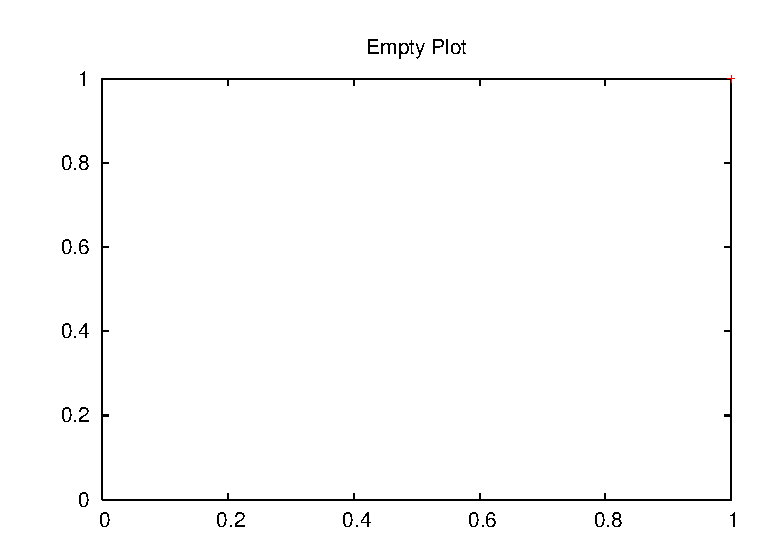
\includegraphics[height=1in]{F/empty.eps}
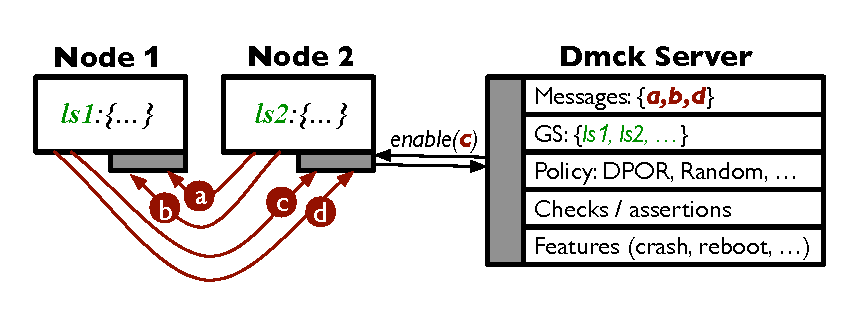
\includegraphics[height=2in]{F/dmck/dmck.eps}
}
\vminfive
\mycaption[Distributed System Model Checker]{fig-dmck}{DMCK}{The figure illustrates a typical framework
of a distributed system model checker (dmck).
}
%\vminten
\end{figure}

\if 0
The figure shows a dmck server model checking
a target distributed system containing two nodes.  
Communications in the target system are interposed 
\fi


The last ten years have seen a rise of software model checker that checks
distributed systems directly at the implementation level.  Figure~\ref{fig-dmck}
illustrates a dmck integration to a target distributed system, a simple
representation of existing dmck frameworks~\cite{Guo+11-Demeter,
Killian+07-LifeDeathMaceMC, Simsa+10-Dbug, Yang+09-Modist}.  The dmck inserts an
interposition layer in each node of the target system with the purpose of
controlling all important events (\eg, network messages, timeouts) and
preventing the target system to process the events until the dmck enables them.
A main dmck mechanism is the permutation of events; the goal is to push the
target system into all possible ordering scenarios.  For example, the dmck can
enforce \ts{abcd} ordering in one execution, \ts{bcad} in another, and so on.

\subsection{Symbolic Execution}
% symbolic execution ...
Symbolic execution is another powerful formal method to verify systems
correctness.  Symbolic execution also faces an explosion problem, specifically
the path explosion problem.  A huge body of work has successfully addressed the
problem and made symbolic execution scale to large (non-distributed) software
systems \cite{Bucur+11-ParallelSymEx, Cadar+08-KLEE, Chipounov+11-S2e,
Cui+13-RuleDirectedSymExec, Zamfir+10-Synthesis}.  Symbolic execution and model
checking can formally be combined into a more powerful
method \cite{Burch+92-SymbolicMC}, however this concept has not permeated the
world of distributed systems; it is challenging to track symbolic values across
distributed nodes.

\subsection{Fault Injector}
% fault injector
Reliability bugs are often caused by incorrect handling of
failures \cite{Gunawi+11-FateDestini, Gunawi+08-EIO}.  Fault-injection testing
however is challenging due to the large number of possible failures to inject.
This challenge led to the development of efficient fault-injection testing
frameworks.  For example, AFEX \cite{Banabic+12-Blackbox} and
LFI \cite{Marinescu+10-ExtensibleLFI} automatically prioritize ``high-impact
targets'' (\eg, unchecked system calls).  These novel frameworks target
non-distributed systems and thus the techniques are different than ours.

% distributed systems
Similarly, recent work highlights the importance of testing faults in cloud
systems (\eg, \fate \cite{Gunawi+11-FateDestini}, \setsudo
\cite{Joshi+13-SetsudoTesting}, \prefail \cite{Joshi+11-PreFail}, and OpenStack
fault-injector \cite{Ju+13-FaultResOpenStack}). However, these frameworks are
not a dmck; they cannot re-order concurrent messages and failures and therefore
cannot catch distributed concurrency bugs systematically.


\section{Scalability}
\label{bg-sc}

\subsection{Vertical Scaling vs Horizontal Scaling} 
\label{bg-sc-type}

When systems' workload grows (the number of users raises or individual users'
requests increase), developers need to scale the systems to add more capability
and keep users satisfied. Two traditional approaches to scale system are used as
we show below \cite{Michael+07-ScaleUpXScaleOut}:
\begin{itemize}

\item \textbf{Vertical scaling or scale-up}: this approach expands system
capabilities by adding more resources (\eg, CPU, memory, and storage) to a
single node to boost its performance, and make software to leverage additional
resources. For example, run more processes of applications in the node.

\item \textbf{Horizontal scaling or scale-out}: this approach enhance the
capability by adding more nodes to current distributed systems to yeild higher
aggregate capability; mostly, the nodes that we are adding are low-cost
machines.

\end{itemize}

In the past, vertical scaling was widely favored by many companies.
Multiprocessor with higher clock rate can satisfy computing power need of
largest companies \cite{Michael+07-ScaleUpXScaleOut}. Vertical scaling requires
less human effort than horizontal scaling; it does not need more administrative
effort because the number of machines and systems administrators need to handle
is still the same. The disadvantages of vertical scaling are the upgradability
is limited by existing hardware manufacturing, and the upgrade cost is
expensive.

Because of the upgradability and price issues, nowadays, the trend goes to
horizontal scaling. Many cloud service companies adopt this approache (\eg,
Google, Facebook, Amazon, \etc). The cost of horizontal scaling is much more
cheaper than the vertical scaling and there is not limitation for hardware to
scale out infinitely (the limitations are posed by software stack)
\cite{ScaleUpVsScaleOut}. In addition, hardware manufaturers try to facilitate
scale-out approach \cite{Michael+07-ScaleUpXScaleOut}.

\subsection{Scalability Testing}

As we discussed in \ref{bg-sc-type}, horizontal scaling or scale-out is a trend
now because it does not expose hardware limitation. The limitation is in
software stack so developers need to invent scalable algorithms and protocols,
however, before real deployment, if they do not have a large cluster to test
their implementations, there could be ``scalability bugs'' hide there.

We now discuss popular approaches (simulation, extrapolation, and emulation) for
unearthing scalability bugs that avoid acquiring a number of machines, because
testing on such deployments is costly.
% ......
First, simulation approaches test system/application models in different scales
\cite{Calotoiu+13-ApmScaleBug, Laguna+15-DebugAtScale}, However, a model can
look scalable but the actual implementation can contain unforeseen bugs. Later
in Section \ref{chp-scb}, we will show our observations from \textit{real world}
scability bugs that simulation cannot detect them.

Second, extrapolation monitors system behaviors in ``mini clusters'' and
extrapolates them to larger scales (\sec2.1 in \cite{Wang+14-Exalt}). However,
mini clusters tend to be order(s) of magnitude smaller than real deployments.
Most importantly, system behaviors do not always extrapolate linearly
\cite{Wang+14-Exalt}. 

Finally, real-scale emulation checks real implementations in an emulated
environment \cite{Gupta+08-DieCast, Wang+14-Exalt}. This approach emulates real
large-scale system in a single machine. For example, a naive way to achieve this
is just colocating multiple processes/VMs on one machine. The limitation here is
emulation consumes real resources (CPU, memory, and storage), so with limited
resources, we can not emulate \textit{really large} deployment (\eg, can test up
to 50-node deployment). Some works try to resolve this resource contention issue
\cite{Gupta+08-DieCast, Wang+14-Exalt}. We will discuss them in related work
(Section \ref{xxx}).

\subsection{Scalability Benchmarking}

Scalability benchmarking (\eg, YCSB~\cite{Cooper+10-YCSB}) is a standard method
to check throughput/latency scalability.  The results are useful for
advertising system capabilities, and thus acquiring a large number of machines
is justifiable.  Debugging code however is a different matter; for every
scalability bug, developers need to debug the code in tens/hundreds of
iterations.  A single-machine debugging approach is valuable.

%\section{Related Work}
\label{bg-related}

\section{Conclusion}

In this chapter, we discuss about cloud-scale distributed systems, software
backend for the cloud computing. We show what the current trend of the systems
is and how they are design. We also discuss about distributed concurrency and
scalability, the two important aspects of cloud-scale distributed systems that
could threaten dependability of the systems. We briefly discuss how system
community address issues from the concurrency and scalability. Unfortunately,
distributed concurrency bugs are still an unsolved problem, and scalability bugs
are novel and not many works address about them.



\chapter{\taxdc: A Taxonomy of Non-Deterministic Concurrency Bugs in Cloud
Distributed Systems}

%\section{Introduction}
%\label{sec-intro}

Concurrency bugs are one notorious type of software bugs that happen in
concurrency systems. These timing-related bugs manifest non-deterministically,
and hence are extremely difficult to detect, diagnose, and fix. A huge body of
work exists in this space that focuses on ``local'' concurrency (LC) bugs in
single-machine multi-threaded software, caused by incorrect interleaving of
memory accesses. And for cloud-scale distributed systems, the reliability is
also severely threatened by non-deterministic concurrency bugs as well, which we
refer as {\em distributed concurrency (DC) bugs}. Distributed systems execute
many complicated distributed protocols on hundreds/thousands of machines with no
common clocks, and must face a variety of random hardware failures
\cite{Do+13-Limplock, Gunawi+14-Cbs}. This combination makes distributed
systems prone to DC bugs caused by non-deterministic timing of distributed
events such as message arrivals, node crashes, reboots, and timeouts. These DC
bugs cannot be directly tackled by LC bug techniques, and they cause fatal
implications such as operation failures, downtimes, data loss and
inconsistencies.

Fighting DC bugs is challenging, particularly given the preliminary
understanding of real-world DC bugs.  To make progress, a comprehensive bug
study is needed. Past studies have closely examined bugs in various software
systems \cite{Chou+01-Empirical, Lu+13-FsEvolution, linux.asplos11}, which have
motivated and guided many aspects of reliability research.
%
There are few bug studies on cloud-scale distributed systems
\cite{Gunawi+14-Cbs, Li+13-ScopeBugStudy}, but they did not specifically dissect
DC bugs. There was an internal bug study dissecting network-failure-related DC
bugs to be a foundation to combat those bugs, but it was not published
\cite{Joshi+13-SetsudoTesting}, and one recent work analyzed non-determinism in
MapReduce programs but only discussed five bugs \cite{Xiao+14-NonDetMR}.
%
Thorough studies have also been conducted for LC bugs \cite{study.dsn10,
Lu+08-ConcurrencyBugStudy} with many follow-up work to date, yet {\em there is
no comprehensive study on real-world distributed concurrency bugs}. We fill this
void in this chapter by presenting our in-depth analysis of \numDcBugs\ DC bugs.
The bugs came from four popular datacenter distributed systems: Cassandra
\cite{CassandraWeb}, HBase \cite{HBaseWeb}, Hadoop MapReduce \cite{HadoopWeb},
and ZooKeeper \cite{ZooKeeperWeb}.
%
We introduce \taxdc, a comprehensive taxonomy of real-world DC bugs across
several axes of analysis such as the triggering timing condition and input
preconditions, error and failure symptoms, and fix strategies, as shown in
detail in Table \ref{tab:tax}.



\section{TaxDC}
\label{sec-taxdc}

In this formal study on DC bugs, we do in-depth analysis of \numDcBugs\ DC
bugs.  The bugs came from four popular cloud distributed systems: Cassandra
\cite{CassandraWeb}, HBase \cite{HBaseWeb}, Hadoop MapReduce \cite{HadoopWeb},
and ZooKeeper \cite{ZooKeeperWeb}.
%
We introduce \taxdc, a comprehensive taxonomy of real-world DC bugs across
several axes of analysis such as the triggering timing condition and input
preconditions, error and failure symptoms, and fix strategies, as shown in
detail in Table \ref{tab:tax}.

As the main contribution, \tdc\ will be the first large-scale DC-bug benchmark.
In the last six years, bug benchmarks for LC bugs have been released
\cite{Jalbert11-RADBench, jieyu}, but no large-scale benchmarks exist for DC
bugs.  Researchers who want to evaluate the effectiveness of existing or new
tools in combating DC bugs do not have a benchmark reference.  \tdc\ provides
researchers with more than 100 thoroughly taxonomized DC bugs to choose from.
Practitioners can also use \tdc\ to check whether their systems have similar
bugs.  The DC bugs we studied are considerably general, representing bugs in
popular types of distributed systems.

As a side contribution, \tdc\ can help open up new research directions. In the
past, the lack of understanding of real-world DC bugs has hindered researchers
to innovate new ways to combat DC bugs.  The state of the art focuses on three
lines of research: monitoring and postmortem debugging \cite{Geels+07-Friday,
Liu+08-D3S, Liu+07-WiDS, Reynolds+06-Pip}, testing and model checking
\cite{Guo+11-Demeter, Killian+07-LifeDeathMaceMC,
Simsa+10-Dbug, Yang+09-Modist}, and verifiable language frameworks
\cite{Desai+13-PLang, Wilcox+15-Verdi}.  We hope our study will not only improve
these lines of research, but also inspire new research in bug detection tool
design, runtime prevention, and bug fixing, as elaborated more in Section
\ref{sec-less}.




\section{Methodology}
\label{sec-met}

%\myquote{``I'm suspecting there is a race condition.'' --- \zk{1496}}


% -------------------------------------------------
\vfifteen
\subsection{Basic Definitions}
\label{met-def}

A {\em distributed concurrency (DC) bug} is a 
concurrency bug in distributed
systems caused by distributed events that can occur in
non-deterministic order.  An {\em event} can be a message arrival/sending, 
local computation, fault, and reboot.
%
A {\em local concurrency (LC) bug} is a 
concurrency bug that happens locally
within a node due to thread interleaving.
%
In our model, a {\em distributed system} is a collection of
shared-nothing nodes.  Each node can run multiple protocols in
multiple threads.
%


% -------------------------------------------------
\subsection{Target Systems and Dataset}
\label{met-data}


Our study examined bugs from four widely-deployed
open-source datacenter distributed
systems that represent a diverse set of system architectures: Hadoop
MapReduce (including Yarn) \cite{HadoopWeb} representing distributed
computing frameworks, HBase \cite{HBaseWeb} and Cassandra
\cite{CassandraWeb} representing distributed key-value stores (also
known as NoSQL systems), and ZooKeeper \cite{ZooKeeperWeb}
representing synchronization services.
%
They are all fully complete systems containing many complex concurrent
protocols.  Throughout the chapter, we will present short examples of DC
bugs in these systems.  Some detailed examples are illustrated in Figure
\ref{fig-zook}, \ref{fig-paxos} and \ref{fig-hbase}.

The development projects of our target systems are all hosted under
Apache Software Foundation wherein organized issue repositories (named
``JIRA'') are maintained.  To date, across the four systems, there are
over 30,000 issues submitted.  One major challenge is that issues
pertaining to DC bugs do not always contain plain terms such as
``concurrency'', ``race'', ``atomicity'', \etc\ Scanning all the
issues is a daunting task.  Thus, we started our study from an open
source cloud bug study (CBS) database \cite{CBSWeb}, which already
labels issues related to concurrency bugs.  However, beyond simple
labeling, the CBS work did not differentiate DC from LC bugs and did
not dissect DC bugs further.

From CBS, we first filtered out LC bugs, then exclude 
DC bugs that do not contain clear description, and finally
randomly picked \numDcBugs\ samples
from the remaining detailed DC bugs, specifically \numDcCA\
Cassandra, \numDcHB\ HBase, \numDcMR\ Hadoop MapReduce, and \numDcZK\
ZooKeeper DC bugs, reported in January 2011-2014 (the time range of
CBS work).  
We have seen much fewer clearly explained DC bugs in CBS from 
Cassandra and ZooKeeper than those from HBase and Hadoop MapReduce, which 
may be related to the fact that they are different types of distributed
systems.  For example,  ZooKeeper, as a
synchronization service, is quite robust as it is built on the
assumption of event asynchrony since day one. Cassandra was built on
eventual consistency, and thus did not have many complex transactions,
until recently when Cassandra adopts Paxos.  We still see new DC bugs
throughout 2014-2015 (some pointed to us by the developers); they can
be included into \tdc\ in the future.




% ---------------------------------
\subsection{Taxonomy}
\label{met-tax}


\definecolor{Gray}{gray}{0.75}
\begin{table}[!htb]
%\footnotesize
\centering
\begin{tabular}{lp{5.5in}}
\toprule
%\rowcolor{Gray}
\multicolumn{2}{c}{{\bf Triggering} }\\
\midrule
\multicolumn{2}{l}{\it What is the triggering timing condition?}\\
&{Message arrives unexpectedly late/early}\\
&{Message arrives unexpectedly in the middle}\\
&{Fault (component failures) at an unexpected state}\\
&{Reboot at an unexpected state}\\
\multicolumn{2}{l}{\it What are the triggering inputs preconditions?}\\
 & {Fault, reboot, timeout, background protocols, and others}\\ 
%&{\scriptsize Node/Job crash}\\
%&{\scriptsize Node/Job restart after crash}\\
%&{\scriptsize Node/Job shut-down}\\
%&{\scriptsize Node/Job start-up}\\
%&{\scriptsize Time out}\\
%&{\scriptsize Others (e.g., client requests)}\\
\multicolumn{2}{l}{\it What is the triggering scope?}\\
&{\it How many nodes/messages/protocols are involved?}\\
\midrule
%\rowcolor{Gray}
\multicolumn{2}{c}{{\bf Errors \& Failures} }\\
\midrule
\multicolumn{2}{l}{\it What is the error symptom?}\\
&{Local memory exceptions}\\
&{Local semantic error messages \& exceptions}\\
&{Local hang}\\
&{Local silent errors (inconsistent local states) }\\
&{Global missing messages}\\
&{Global unexpected messages}\\
&{Global silent errors (inconsistent global states)}\\
\multicolumn{2}{l}{\it What is the failure symptom?}\\
&{Node downtimes, data loss/corruption, operation failures, slowdowns}\\
\midrule
%\rowcolor{Gray}
\multicolumn{2}{c}{{\bf Fixing} }\\
\midrule
\multicolumn{2}{l}{\it What is the fix strategy?}\\
&{Fix Timing: add global synchronization}\\
&{Fix Timing: add local synchronization}\\
&{Fix Handling: retry message handling at a later time}\\
&{Fix Handling: ignore a message}\\
&{Fix Handling: accepting a message without new computation logics}\\
&{Fix Handling: others}\\
\bottomrule
\end{tabular}
\mycaption[Taxonomy of DC Bugs]{tab:tax}{Taxonomy of DC Bugs}{}
\end{table}


We study the characteristics of DC
bugs along three key stages: triggering, errors \& failures, and
fixing (Table \ref{tab:tax}).
%
{\it Triggering} is the process where software execution states
deviate from correct to incorrect under specific conditions.  At the
end of this process, the manifestation of DC bugs changes from
non-deterministic to deterministic.
%
{\it Errors and failures} are internal and external software
misbehaviors.
%
{\it Fixing} shows how developers correct the bug.  We
will discuss in detail these categories in their respective sections.

% -----------------------------------------
\subsection{Threats to Validity}
\label{met-valid}

For every bug, we first ensure that the developers marked it as a real bug (not
a false positive).  We also check that the bug description is clear. Finally, We
then {\em re-enumerate} the full sequence of operations (the ``{\em steps}'') to
a clearer and more concise description such as the ones in Figure
\ref{fig-zook}. 
%
Our study cannot and does not cover DC bugs not fixed by the developers.  Even
for fixed bugs, we do not cover those that are not described clearly in the bug
repositories, a sacrifice we had to make to maintain the accuracy of our
results.  

Readers should be cautioned not to generalize the statistics we report as each
distributed system has unique purpose, design and implementation.
%
For example, we observe 2:1 overall ratio between order and atomicity violations
\sec\ref{trig-time}, however the individual ratios are different across the four
systems (\eg\ 1:2 in ZooKeeper and 6:1 in MapReduce).  
%
Like all empirical studies, our findings have to be interpreted with our
methodology in mind.

%\vfive % for good spacing

% -----------------------------------------
\subsection{TaxDC Database}
\label{met-db}

We name the product of our study \tdc\ database.  \tdc\ contains in
total \numTagsAll\ classification labels and \numDescLOC\ lines of
clear and concise re-description of the bugs (our version, that we
manually wrote) including the re-enumeration of the steps, triggering
conditions, errors and fixes.
%
We release \tdc\ to the public
\footnote{\url{http://ucare.cs.uchicago.edu/project/taxDC}}.  We believe \tdc\
will be a rich ``bug benchmark'' for researchers who want to tackle distributed
concurrency problems.  They will have sample bugs to begin with, advance their
work, and do not have to repeat our multi-people-year effort.


\vfive % for good spacing

% -----------------------------------------
\subsection{Detailed Terminologies}
\label{met-pres}

% ----------------- state
Below are the detailed terminologies we use in this chapter.
% basics
We use the term ``state'' to interchangeably imply {\em local state}
(both in-memory and on-disk per-node state) or {\em global state}
(a collection of local states and outstanding messages).
%
A {\em protocol} (\eg, read, write, load balancing) creates a chain of
events that modify system state.
%
User-facing protocols are referred as {\em foreground} protocols while
those generated by daemons or operators are referred
as {\em background} protocols.


% ------------------- fault
We consider four types of {\em events}: message, local computation,
fault and reboot.  The term {\em fault} represents component failures
such as crashes, timeouts, and disk errors.
%
A {\em timeout} (system-specific) implies a network disconnection
or busy peer node.
%
A {\em crash} usually implies the node experiences a power failure. %and does
%not come back up.
%
A {\em reboot} means the node comes back up.


% ---------------------------- DC bug presentation
Throughout the chapter, we present bug examples by abstracting
system-specific names.  As shown in Figure \ref{pat}, we use capital
letters for nodes (\eg, A, B), two small letters for a message between
two nodes (\mab\ is from A to B).  Occasionally, we attach
system-specific information in the subscript (\eg, A\sub{AppMaster}
sends \mab\sub{taskKill} message to B\sub{NodeManager}).
%
We use \underline{`` \textbf{/} ''} to imply concurrency
(\mac\ss\mbc\ implies the two messages can arrive at C in different
orders, \mac\ or \mbc\ first).
%
A dash, \underline{`` {\bf --} ''}, means causal relation of two
events (\mab-\mbc\ means \mab\ causally precedes\ \mbc).
%
Finally, we use \underline{``N{\bf *}''} to represent crash,
\underline{``N{\bf !}''} reboot, and \underline{``N{\bf +}''} local
computation at N.


% -------------------------- issue citation
We cite bug examples with clickable hyperlinks (\eg, \mr{3274}).
%
To keep most examples uniform, we use MapReduce examples whenever
possible.
%
%For interested readers, we cite more examples in the 
%footnotes (\eg, \spa\spb\spc).
%
%
We use the following abbreviations for system names:
``c/CA'' for Cassandra,
``h/HB'' for HBase, 
``m/MR'' for Hadoop MapReduce, and
``z/ZK'' for ZooKeeper;
% 
and for system-specific components:
``AM'' for application master,
``RM'' for resource manager,
``NM'' for node manager, 
``RS'' for region server, and
``ZAB'' for ZooKeeper atomic broadcast.



\section{Trigger}
\label{sec-trig}

DC bugs often have a long triggering process, with many local and
global events involved.  To better reason about this complicated process,
we study them from two
perspectives:

\begin{enumerate}

\item
{\em Timing conditions} (\sec\ref{trig-time}): For every DC bug, we
identify the smallest set of concurrent events $E$, so that a specific
ordering of $E$ can guarantee the bug manifestation.  This is similar
to the interleaving condition for LC bugs.



\item
{\em Input preconditions} (\sec\ref{trig-input}): In order for those
events in $E$ to happen, regardless of the ordering, certain inputs or
fault conditions (\eg, node crashes) must occur.  This is similar to the
input condition for LC bugs.

\end{enumerate}
%
Understanding the triggering can help the design of testing tools
that can proactively trigger DC bugs, bug detection tools that 
can predict which bugs can be triggered through program analysis,
and failure prevention tools that can  sabotage the triggering
conditions at run time.






% ===============================================
\subsection{Timing Conditions (TC)}
\label{trig-time}


Most DC bugs are triggered either by untimely delivery of messages,
referred to as {\it message timing bugs}, or by untimely faults or
reboots, referred to as {\it fault timing bugs}.  Rarely DC bugs are
triggered by both untimely messages and untimely faults, referred to
as {\it message-fault bugs}.  Table \ref{tab:trig} shows the
per-system breakdown and Figure \ref{bars}a (\BTMC) the overall
breakdown.  Since a few bugs are triggered by more than one type of
timing conditions
(\sec\ref{trig-scope}), the sum of numbers in Table \ref{tab:trig} is
slightly larger than the total number of DC bugs.

% ----------------------------
\paragraph{Message Timing Bugs.}

The timing conditions can be abstracted to two categories:


\begin{enumerate}[label=\alph*.]
%\begin{enumerate}

\item 
{\em Order violation} (\pctTrigOrder\ in Table \ref{tab:trig}) means 
a DC bug manifests
whenever a message comes earlier (later) than another event, which is
another message or a local computation, but not when the message comes
later (earlier).

\item
{\em Atomicity violation} (\pctTrigAtom\ in Table \ref{tab:trig}) 
means a DC bug manifests
whenever a message comes in the middle of a set of events, which is a
local computation or global communication, but not when the message
comes either before or after the events.

\end{enumerate}
%
LC and DC bugs are similar in that their timing conditions can both be
abstracted into the above two types. However, the subjects in these
conditions are different: shared memory accesses in LC and message
deliveries in DC. The ratio between order violation and atomicity
violation bugs are also different:
previous study of LC bugs showed that
atomicity violations are much more common than order violations in practice
%
\cite{Lu+08-ConcurrencyBugStudy}; 
our study of DC bugs 
shows that this relationship does not apply or even gets reversed
in several representative distributed systems.
%
%
%




\begin{table}[t]
\small
\centering
\begin{tabular}{lcccc}
\toprule
   & Ordering & Atomicity & Fault & Reboot \\
\midrule
CA &  4  & 4 & 6 & 5 \\
HB &  13  & 9 & 8 & 1 \\
MR & 25  & 4 & 5 & 3 \\
ZK &  4  & 8 & 7 & 5 \\
\midrule
All &  46  & 25 & 26 & 14 \\
\bottomrule
\end{tabular}

\mycaption{tab:trig}{\#DC bugs triggered by timing conditions
(\sec{\ref{trig-time}})}{The total is more than \numDcBugs\ because some bugs
require more than one triggering condition. More specifically, 46 bugs 
(\pctTrigOrder) are caused {\em only} by 
ordering violations, 21 bugs (\pctTrigAtom) 
{\em only} by atomicity violations, and 4 bugs (\pctTrigMix) by multiple timing 
conditions (as also shown in Figure \ref{bars}a).}

\end{table}

 %----tab


\if 0
\jirafootnote{trig-time}{tab:trig}{
\spa \ca{5631}, \hb{4015}, \mr{3006}, \zk{1144};  % order violation
\spb \ca{1011}, \hb{4729}, \mr{5198}, \zk{1496};  % atomicity violation
\spc \ca{6415}, \hb{5806}, \mr{4819}, \zk{1653};  % crash timing
\spd \ca{2083}, \hb{6317}, \mr{5489}, \zk{975}.  % reboot timing
%
--- These examples are clickable hyperlinks pointing to 
\href{https://issues.apache.org/jira/browse/MAPREDUCE-3006}{https://issues.apache.org/jira/browse/S-NUM} where ``S'' and
``NUM'' are the system name and the issue number respectively.
For example, \mr{3006} points to 
\href{https://issues.apache.org/jira/browse/MAPREDUCE-3006}{https://issues.apache.org/jira/browse/MAPREDUCE-3006}.
}
\fi



% message-message
An order violation can originate from a race between two messages
({\em message-message race}) at one node.  The race can happen between
two message arrivals.  For example, Figure \ref{pat}a illustrates
\mac\ss\mbc\ race at node C in \mr{3274}.  Specifically, B\sub{RM}
sends to C\sub{NM} a task-init message (\mbc\sub{init}), and soon
afterwards, A\sub{AM} sends to C\sub{NM} a task-kill preemption
message (\mac\sub{kill}), however \mac\sub{kill} arrives {\em before}
\mbc\sub{init} and thus is incorrectly ignored by C.  The bug would
not manifest if \mac\sub{kill} arrives {\em after} \mbc\sub{init}
(Figure \ref{pat}b).
%
Message-message race can also happen between a message arrival and a
message sending.  For example, the \mab\ss\mbc\ race in Figure
\ref{pat}c depicts \hb{5780}.  In this bug, B\sub{RS} sends to
C\sub{Master} a cluster-join request (\mbc\sub{join}) unexpectedly
{\em before} a security-key message (\mab\sub{key}) from A\sub{ZK}
arrives at B, causing the initialization to abort.

Interestingly, message-message race can also occur concurrently across
two nodes.  For example, Figure \ref{pat}d illustrates
\mab\ss\mba\ race crisscrossing two nodes A and B in
\mr{5358}.  Specifically, A\sub{AM} sends \mab\sub{kill} to a backup
speculative task at B\sub{NM} because the job has completed, but
concurrently the backup task at B sends \mba\sub{complete} to A,
creating a double-complete exception at A.  If \mab\sub{kill} arrives
early at B, \mba\ will not exist and the bug will not manifest (Figure
\ref{pat}e).

% message-compute
An order violation can also originate from a race between a message
and a local computation ({\em message-compute race}).  For example,
Figure \ref{pat}f illustrates \mab\ss\lbp\ race in \mr{4157}.  First,
B\sub{AM} was informed that a task has finished and B plans to close
the job and remove its local temporary files (\lbp). However, just
{\em before} \lbp, A\sub{RM} sends to B a kill message (\mab) and
hence the files are never removed, eventually creating space issues.
To prevent the failure, the kill message has to arrive after the local
cleanup (Figure \ref{pat}g).


% atomicity violations
An atomicity violation, as defined above, originates when a message
arrives in the middle of a supposedly-atomic local computation or
global communication.
%
For example, Figure \ref{pat}h illustrates \mr{5009}.
When B\sub{NM}
is in the middle of a commit transaction, transferring task output
data (\mbc) to C\sub{HDFS},  A\sub{RM} sends a kill
preemption message (\mab) to B, preempting the task without resetting
commit states on C.
The system is never able to finish the commit --- when B
later reruns the task and tries to commit to C (\mbc'), C throws a
double-commit exception.  This failure would not happen if the kill
message (\mab) comes before or after the commit transaction
(\mbc).





\begin{figure}[t]

\centerline{
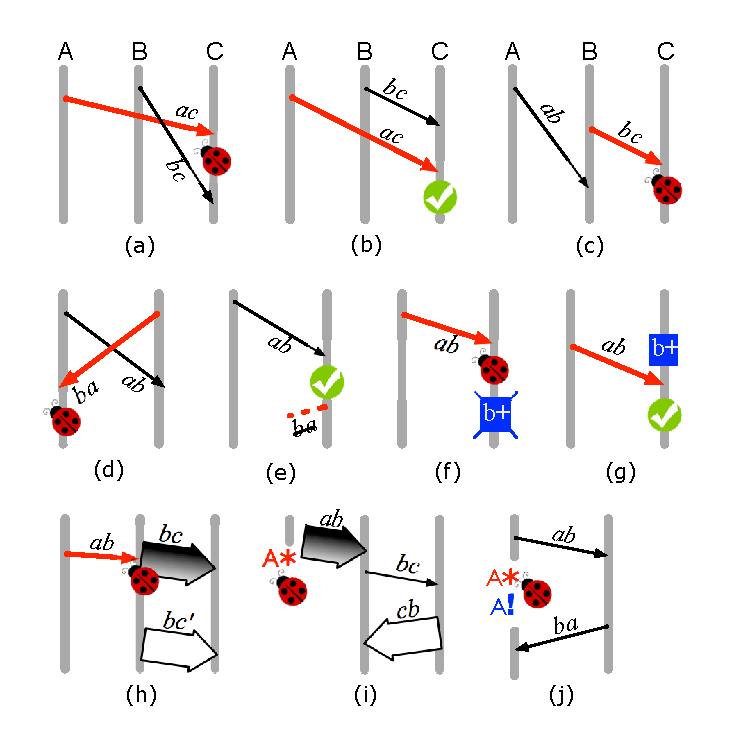
\includegraphics[width=3.5in]{F/patterns/basics.eps}
%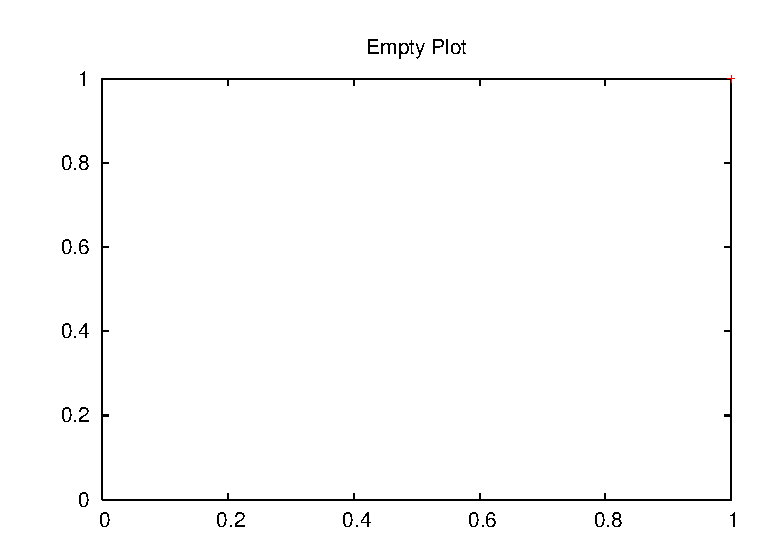
\includegraphics[width=0.5\textwidth]{F/empty.eps}
}
\vminten
\mycaption{pat}{Triggering patterns (\sec{\ref{trig-time}})}
{The three vertical lines represent the timeline of nodes A, B and C.
An arrow with \ts{xy} label implies a message from X to Y.  A square
box with label \ts{x+} implies a local state-modifying computation at
node X.  A thick arrow implies a set of messages performing an atomic
operation.  \ts{X*} and \ts{X!} implies a crash and reboot at node X
respectively (\sec\ref{met-pres}). All figures  are discussed in
\sec{\ref{trig-time}}}

\end{figure}



\if 0
\newtxt{The three lines represent
timeline of nodes A's, B's, and C's events (\ie\ sending/receiving
messages, local computations, crashes/reboots). Arrow lines ac mean
messages from A to C. Square boxes b+ mean local computations in B.
Thick arrows mean a set of messages doing an atomic operation. A*
means a crash of A, and A! means a reboot of A.  Figure (a)
illustrates an order violation pattern due to a race of two message
arrivals on node C (\ie\ messages ac/bc), which the bug would not
manifest if C receives the messages as in figure (b). Figures (c) and
(d) illustrate order violations between a message arrival and a
message sending (\ie\ ab/bc in (c), and ab/ba in (d)) which the bugs
would not happen if B receives the message ab before it sends a
message as in figure (e). Figure (f) illustrates an order violation
pattern between a message arrival and a local computation (\ie\ ab/b+)
which the bug would not manifest, if ab arrives after B has finished
b+ computation as in figure (g). Figure (h) illustrates an atomicity
violation that a message ab comes during B is doing an atomic
operation. Figure (i) illustrates a fault-timing pattern that A
crashes during an atomic operation (\ie\ A*/ab). Figure (j)
illustrates a reboot timing pattern that A crashes and reboots during
B processing a message ab, and A does not expect a message ba; the bug
would not happen if B tries to send ba and finds out A is dead. } }
\fi
 %----fig



% -------------------------
\paragraph{Fault and Reboot Timing Bugs.}

Fault and reboot timing bugs (\pctTrigFR\ in Table \ref{tab:trig})
manifest when faults and/or
reboots occur at specific global states $S$\sub{i}; the bugs do not
manifest if the faults and reboots happen at different global states
$S$\sub{j}. 

Figure \ref{pat}i illustrates a fault-timing bug in \mr{3858}.  Here,
A\sub{NM1} is sending a task's output to B\sub{AM} (\mab) but A
crashes in the middle (A*) leaving the output half-sent. 
The system is then unable to recover from this untimely crash --- B
detects the fault and reruns the task at C\sub{NM2} (via \mbc) and
later when C re-sends the output (\mcb), B throws an exception.  This
bug would not manifest, if the crash (A*) happens before/after
the output transfer (\mab).

Figure \ref{pat}j depicts a reboot-timing bug in \mr{3186}.  Here,
A\sub{RM} sends a job (\mab) to B\sub{AM} and while B is executing the
job, A crashes and reboots (A*, A!)  losing all its in-memory job
description.  Later, B sends a job-commit message (\mba) but A throws
an exception because A does not have the job information.  The bug
would not manifest if A reboots later: if A is still down when B sends
\mba\sub{commit} message, B will realize the crash and cancel the job before
A reboots and A will repeat the entire job assignment correctly.






%\newcommand{\fev}[1]{\textcolor{Maroon}{\textit{#1}}}
%\newcommand{\ev}[1]{\textcolor{gray}{\textbf{#1}}}


\begin{figure}[t]
\centering
\footnotesize
\begin{tabular}{|p{3.2in}|} 
% ---------------------------------------------------- Sample
\hline
{\bf \zk{1264}:}
\ev{(1)} \fev{Follower F crashed} in the past,
\ev{(2)} \fev{F reboots} and joins the cluster,
\ev{(3)} Leader L sync data with F and send snapshot, 
\ev{(4)} \fev{In the middle of step 3-6},
% Before syncing finishes (in step 6), 
client updates data with Tx-\#15; L forwards the update to F,
\ev{(5)} F applies the update in memory only, due to a concurrent sync,
\ev{(6)} L tells F syncing is finished, % \fev{after step 5},
\ev{(7)} Client updates data with Tx-\#16; F writes update to disk correctly,
\ev{(8)} \fev{F crashes},
\ev{(9)} \fev{F reboots} and joins the cluster again,
\ev{(10)} L sync data with F, but this time L sends only ``diff'' starting with Tx-\#17
\ev{(11)} F permanently \fev{loses data} from Tx-\#15,
inconsistent with L and other followers!
% \ev{(12)} Violaton: permanent data inconsistency as F does not have data from txid \#15,
\\ \hline
% ----------------------------------------------------
\end{tabular}
%---------------------------------
\vminfive
\mycaption{fig-zook}{A DC bug in ZooKeeper}{}
\end{figure}



%\ev{(5)} L forwards the update request txid \#15 to F,

% ---------------------------------------------------- CA simple
% ---------------------------------------------------- CA complex
% ---------------------------------------------------- HBase simple
% ---------------------------------------------------- HBase complex
% ---------------------------------------------------- MR simple
% ---------------------------------------------------- MR complex
% ---------------------------------------------------- ZK simple
% ---------------------------------------------------- ZK complex




\paragraph{Message-Fault Bugs.}
Four DC bugs are caused by a combination of messages and faults. 
For example, in Figure
\ref{fig-zook}, a message (step 4) arrives in the middle of some
atomic operation (step 3-6). This message atomicity violation leads
to an error that further requires a fault timing (step 8) to become an
externally visible failure.



\finding{DC bugs are triggered mostly by 
\textit{untimely messages} (\pctTrigMsg\ in Table \ref{tab:trig}) 
and % $\sim$70\%
sometimes by \textit{untimely faults/reboots} (\pctTrigFR), % $\sim$30\% 
and occasionally by a \textit{combination} of both (\pctTrigMix). % $<$5\%
Among untimely messages, two thirds commit order violations 
% Some untimely messages commit order violations (\pctTrigMsgOrder), %\sim$60
due to message-message or message-computation race on the node they arrive;
%(Figure\ref{pat}a--g);
the others commit atomicity violations.}
%(Figure\ref{pat}h).}

%These patterns provide
%important guidance to future research in combating DC bugs
%(\ref{sec-sol}).
%}




% ===============================================
\subsection{Input Preconditions (IP)} 
\label{trig-input}


The previous section presents simple timing conditions that can be
understood in few simple steps.  In practice, many of the conditions
happen ``deep'' in system execution.  In other words, the triggering
path is caused by complex input preconditions (IP) such as faults, reboots,
and multiple protocols.  Let's use the same example in Figure
\ref{fig-zook}.
%
First, a fault and a reboot (step 1-2) and a client request (step 4)
must happen to create a path to the message atomicity violation (step
4 interfering with step 3-6).
%
Second, conflicting messages from two different protocols (ZAB and
NodeJoin initiated in step 2 and 4) have to follow specific
bug-triggering timing conditions.
%
Even after the atomicity violation (after step 6), the bug is not
guaranteed to lead to any error yet (\ie, a benign race).
%
Finally, the follower experiences an untimely fault (step 8), such
that after it reboots (step 9), a global replica-inconsistency error
will happen (step 11).
%
Put it in a reverse way, before step 8, the global state is $S$\sub{i}
and $S$\sub{i}$+$crash$\rightarrow$error, and the only way for the
system to reach $S$\sub{i} is from complex preconditions such as a
fault, a reboot, and some foreground and background protocols.



Statistically, Figure \ref{bars}b (\BFLT) shows that \pctFaultYes\ of
DC bugs must have at least one fault.  In more detail, Figure
\ref{bars}c-e (\BTO, \BCR, \BRB) shows the percentage of issues that
require timeouts, crashes and reboots respectively, including how many
instances of such faults must be there; the rest is other faults such
as disk errors (not shown).


Figure \ref{bars}f (\BPROT) shows how many ``protocol initiations''
mentioned in the bug description.  For example, if the system needs to
perform one execution of background protocol and also three concurrent
calls to the \ts{write} protocol, then we label it with four protocol
initiations.  Up to 3 protocol initiations covers three quarters of
DC bugs.
%
When we count the number of {\em unique} protocols involved in all the
bugs we study, we record \totProtCA\ Cassandra, \totProtHB\ HBase,
\totProtMR\ MapReduce, \totProtZK\ ZooKeeper unique protocols, or
\totProtAll\ protocols in total.  This again highlights the complexity
of fully complete systems.
%
Figure \ref{bars}g (\BBFG) shows our categorization of protocols that
are concurrently running into foreground only,
background only, and foreground-background (mix)
categories.  More than three quarters of the bugs involve some
background protocols and about a quarter involves a mix of foreground
and background protocols.

\finding{Many DC bugs need \textit{complex input preconditions}, 
such as faults
(\pctFaultYes\ in Figure \ref{bars}b), multiple protocols
(\pctProtMany\ in Figure \ref{bars}f), and background protocols 
(\pctProtBg\ in Figure \ref{bars}g) .}




\begin{figure}

\centerline{
\begin{tikzpicture}[font=\sffamily\footnotesize]
\begin{axis}[
xbar stacked,
y=0.8cm,
%width=5in,
width=\columnwidth,
%height=120pt,
xmin=0,
xmax=100,
bar width=12pt,  
%xmajorgrids=true,
%ylabel={Categorizations},
symbolic y coords={RB, CR, TO, FLT},
ytick=data,
yticklabels={{(d) RB, (c) CR, (b) TO, (a) FLT}},
every axis y label/.style={at={(ticklabel cs:0.5)},rotate=90,anchor=near ticklabel},
xticklabels={,,},
axis x line*=none,
x axis line style={opacity=0},
axis y line*=right
]
\input{data-bars}
\end{tikzpicture}
%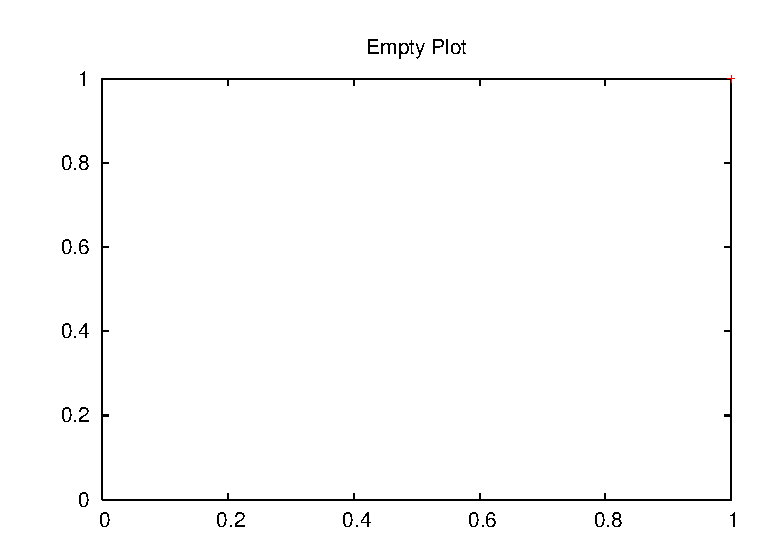
\includegraphics[width=1.8in]{F/empty.eps}
}
\vminten
\mycaption{bars}{Statistical overview of DC bugs}{}
% \vten

\end{figure}


%
\if 0
nodes (TSN), 
protocols (TSP), 
background (BR), 
triggering messages (TSM), 
local-message race (LM), 
timeout (TO),
crashes (CR),
reboots (RB),
errorMessage (EM),
reported (REP),  
implication (IMP),
control/data plane (CDP), 
\fi







\begin{figure*}[t]

\centerline{
%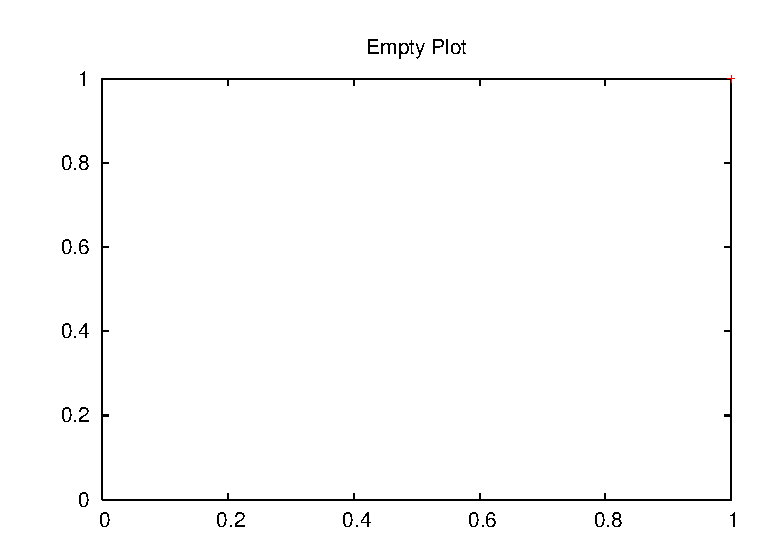
\includegraphics[width=6.5in]{F/empty.eps}
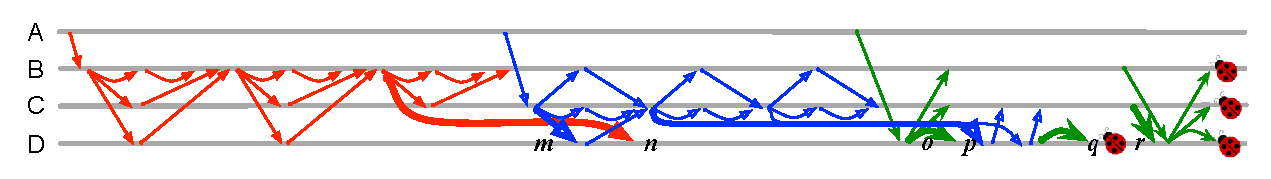
\includegraphics[width=7.0in]{F/paxos/paxos.eps}%
}
\vminfive
\mycaption{fig-paxos}{A Cassandra's Paxos bug}{In \ca{6023}, 
three key-value updates 
(different arrow types)
concurrently execute the Paxos protocol on four nodes
(we simplify from the actual six nodes).
The bug requires three message-message race conditions:
(1) \emph{m} arrives before \emph{n}, 
(2) \emph{o} before \emph{p}, and
(3) \emph{q} before \emph{r}, which collectively
makes D corrupt the data and propagate the corruption
to all replicas after the last broadcast.
Note that the bug would not surface if any of the conditions
did not happen. 
It took us one full day to study this bug.
}
\vten
\end{figure*}

 % --

\if 0
\pctProtMany\ \xxx\ of the bugs must
have at least two different protocols running.  A protocol sometimes
must also be triggered multiple times (\eg, three clients concurrently
run the \ts{write} protocol), but currently we do not track this
number.  
\fi


\vten


% ===============================================
\subsection{Triggering Scope (TS)}
\label{trig-scope}


We now analyze the triggering scope (TS), which is a complexity measure of
DC-bug timing conditions.  We use four metrics to measure the scope:
message count (\BTSM), node (\BTSN), protocol (\BTSP), and untimely
event (\BTSU) counts as shown in Figure \ref{bars}h-k.  This statistic
is important with respect to the scalability of model checking, bug
detection and failure diagnostic tools
(\sec\ref{less-dmck}-\ref{less-diagnose}).

Message count implies the minimum
number of messages involved in $E$ as defined in the beginning of
section \ref{sec-trig}.  Figure \ref{bars}h (\BTSM) shows that one or two
triggering messages are the most common, with 7 messages as the
maximum.  Informally, zero implies fault timing bugs without any
message-related races, one implies message-compute race, two implies
message-message as in Figure \ref{pat}a, and three implies a scenario
such as \mac/(\mab-\mbc) race where \mab\ and \mac\ are concurrent or
non-blocking message sending operations.

The node and protocol scopes present how many nodes and protocols are
involved within the message scope.  Figure \ref{bars}i-j (\BTSN\ and
\BTSP) shows that the scale of node and protocol triggering scope is
also small, mostly two or three nodes and one or two protocols.

The untimely events count implies the total number of order
violations, atomicity violations, untimely faults and reboots in the
triggering timing condition of a bug.  Figure \ref{bars}k
(\BTSU) shows that only eight bugs require more than one untimely
events.  Four of them are message-fault bugs, each 
requiring one untimely message and one
untimely fault to trigger (\eg, step 4 and 8 in 
Figure \ref{fig-zook}).  Three are fault-reboot timing bugs,
each requiring one untimely fault and one untimely reboot.
The last one is \ca{6023}, shown in Figure \ref{fig-paxos}, requiring
three message-message order violations to happen.

%TODO
% --- after the occurrence of 
%the one untimely event, the first error will deterministically propagate to
%failures

\finding{The \textit{timing conditions} of most DC bugs only involve 
\textit{one to three} messages, nodes, and protocols ($>$90\% in
Figure \ref{bars}h-j).  Most DC bugs are mostly triggered by 
only \textit{one} untimely event (\pctTrigScopeUnEvOne\ in Figure 
\ref{bars}k).}
%, which
%is a positive finding for the scalability of
%future bug finding tools (\sec\ref{less-bft}).
%Furthermore, more focus on interactions between foreground
%and background protocols that involve control logic should
%be exercised. 






\section{Errors and Failures}
\label{sec-err}

\subsection{Error Symptoms}
\label{err-err}

% goal
From the triggering conditions, we then scrutinize the {\em first}
error that happens immediately after.  First errors are the pivotal
point that bridges the triggering and error-propagation process.
Identifying first errors help failure diagnosis get closer to
disclosing bug triggering and root causes and help bug detection get
closer to accurately predict failures (\sec\ref{sec-less}).




% our category
We categorize first errors into {\em local} errors and {\em global}
errors, based on whether they can be observed from the triggering node
\nt\ alone.  Here, \nt\ is the node where triggering ends.  It is the
receiver node of untimely messages (\eg, node C in Figure \ref{pat}a)
or the node with untimely fault (\eg, node A in Figure \ref{pat}i).
For each error, we also check whether it is an {\it explicit} or {\em
  silent} error.  
Table \ref{tab:error} and Figure \ref{bars}l
(\BERR) show the per-system and overall breakdowns
respectively. 
Some MapReduce bugs caused multiple concurrent first errors of different types.

\if 0
\jirafootnote{err-err}{tab:error}{
\spa \ca{5925}, \hb{6375}, \mr{5198};  % local memory exception
\spb \hb{4540}, \mr{4607}, \zk{1046};           % local state machine/semantic
\spc \hb{5606}, \mr{4252}, \zk{1144};           % local hangs 
\spd \ca{2590}, \hb{6227}, \mr{4099}, \zk{1382};    % local silent (other than hang)
\spe \ca{1011}, \hb{4015}, \mr{2953};  % global wrong
\spf \ca{5393}, \hb{6060}, \mr{4819};  % global miss
\spg \ca{6023}, \hb{6070}, \zk{962}; % global silent
}
\fi


% local
First, DC bugs can manifest into both local explicit errors and local
silent errors. The former includes
%
{\em memory exceptions} such as null-pointer exceptions
(\pctErrLocMem\ in Table \ref{tab:error}) and {\em semantic errors} 
such as wrong state-machine transition exceptions thrown by 
the software (\pctErrLocSem).
%
Local silent errors include
%
{\em hangs}, such as forever waiting for certain states to change
or certain messages to arrive which are typically observed implicitly
by users (\pctErrLocHang),
%
and {\em local silent} state corruption, such as half-cleaned
temporary files (\pctErrLocSil).




\begin{table}[t]
\small
\centering
\begin{tabular}{lcccccccc}
\toprule
   & \multicolumn{4}{c}{Local Errors} && \multicolumn{3}{c}{Global Errors}\\
\cmidrule{2-5}
\cmidrule{7-9}
   & Mem & Sem & Hang & Sil &    & Wrong & Miss & Sil \\
%   & \spa & \spb & \spc & \spd &    & \spe & \spf & \spg \\
\midrule
CA &  2  & 0 & 0 & 4 & & 3 & 3 & 7  \\
HB &  1  & 2 & 1 & 2 & & 15 & 3 & 6  \\
MR &  2  & 13 & 7 & 4 & & 14 & 4 & 0  \\
ZK &  0  & 6 & 2 & 5 & & 1 & 0 & 5  \\
\midrule
All &  5  & 21 & 10 & 15 & & 33 & 10 & 18  \\
\bottomrule
\end{tabular}
\mycaption{tab:error}{First error symptoms of DC bugs (\sec{\ref{err-err}})}
{Some bugs cause multiple concurrent first errors.}
\end{table}


\if 0
The
abbreviations are the following.
Mem: memory error, Sem: semantic,
Sil: silent,  Miss: missing message, and Wrong: wrong message.
\fi


% global
When local error is non-obvious in \nt, we analyze if the error is
observable in other nodes communicating with \nt.  Many
DC bugs manifest into explicit global errors through {\em wrong
messages} (\pctErrGlobWrong\ in Table \ref{tab:error}). Specifically, 
the communicating
node receives an incorrect message from \nt, and throws an exception
during the message handling.  However, a few DC bugs still lead to
silent global errors. These include {\em missing messages}, where
\nt\ never sends a reply that the communicating node is waiting for
in the absence of timeout (\pctErrGlobMiss), and {\em global
  silent} state corruption such as replica inconsistencies
between \nt\ and the other nodes (\pctErrGlobSil).


\finding{\textit{Local} and \textit{global} first errors are about
equally common; \pctErrLoc\ vs. \pctErrGlob\ in Figure \ref{bars}m
(\BLG).  About half of the DC bugs generate \textit{explicit} first
errors (\pctErrExp), including local exceptions and global wrong
messages, and the remaining DC bugs lead to \textit{silent} errors
(\pctErrImp), as shown in Figure \ref{bars}n (\BES). 
%
Some of them immediately lead to hangs in the triggering node $N_T$
(\pctErrLocHang) or a node communicating with $N_T$
(\pctErrGlobMiss).  }








% =========================================
\subsection{Failure Symptoms}
\label{err-fail}






Figure \ref{bars}o (\BFAIL) shows that errors from DC bugs will
eventually lead to a wide range of fatal failures including
%
node downtimes (\pctFailNode),
data loss/corruption/inconsistencies (\pctFailData),
operation failures (\pctFailOp),
and performance degradation (\pctFailPer).
%
A node downtime happens when the node either crashes or
hangs (\ie, it may still be heartbeating).
It happens to both master/leader nodes and worker/follower nodes
in our study.
%Developers often have a hard
%time in debugging fail-silent behaviors and prefer fail-stop
%behaviors \cite{mr-3634}.
%
Data-related failures and performance problems are an artifact of
incorrect state logic induced from DC bugs.  For example, in HBase,
concurrent region updates and log splittings can cause data loss.
In Cassandra, some dead nodes are incorrectly listed as alive causing
unnecessary data movement that degrades performance.
% 
Node downtimes and data-related failures could also cause some operations
to fail.  To avoid double counting,
we consider a bug as causing operation failures only when it does not cause
node downtimes or data-related failures.

\if 0
\jirafootnotable{err-fail}{
\spa \hb{6153}, \mr{5198}, \zk{1144}; % node down
\spb \ca{2083}, \hb{6227}, \mr{4819}, \zk{1154}; % data loss / stale / corrupt
\spc \ca{5631}, \hb{5780}, \mr{4833}, \zk{1291}; % opfail
\spd \ca{3626}, \hb{5606}, \zk{975}; % perf degrade
}
\fi








\chapter{SAMC: Semantic-Aware Model Checking for Fast Discovery of DC bugs in Cloud Distributed Systems}

%State of the art does not help.

As we discuss in Section \ref{sec-bg-dmck}, a recent popular approach to unearth
DC bugs is adopting distributed system model cheker or dmck. However, due to the
complexity of DC bugs that we discussin Chapter \ref{chp-taxdc} (\eg,
interactions of multiple protocols, and various and multiple faults), the state
of the art of dmcks still cannot work effectively \xxx{cite Modist, dbug,
demeter, macemc}. We observe that the existing systematic reduction policies
cannot find bugs quickly, and cannot scale with the inclusion of fault events.

In this chapter, we discuss how to advance the state of the art by leveraging
semantic awareness to assist model checking, and introduce ``Semantic-Aware
Model Checking'' (SAMC), a white-box model checking approach that takes semantic
knowledge of how events (\eg, messages, crashes, and reboots) are processed by
the target system and incorporates that information in reduction policies. We
first discuss background of dmck and the state of the art in Section \ref{dmck}

%To show the intuition
%behind SAMC, we first give an example of a simple leader election protocol.
%Then, we present SAMC architecture and our four reduction policies.

\section{Semantic Awareness}

In a simple leader election protocol, every node broadcasts its vote to reach a
quorum and elect a leader.  Each node begins by voting for itself (\eg, \ntwo\
broadcasts \ts{vote=2}).  Each node receives vote broadcasts from other peers
and processes every vote with this simplified code segment below.  As depicted
in the code segment below, if an incoming vote is less than the node's current
vote, it is simply discarded.  If it is larger, the node changes its vote and
broadcasts the new vote.

\begin{alltt}
if (msg.vote < myVote) \{
  discard;
\} else \{
  myVote = msg.vote; broadcast(myVote);
\}
\end{alltt}

Let's assume \nfour\ with \ts{vote=4} is receiving three concurrent messages
with votes \ts{1}, \ts{2}, and \ts{3} from its peers.  Here, a dmck with a
black-box DPOR approach must perform 6 (3!) orderings (\ts{123}, \ts{132}, and
so on).  This is because a black-box DPOR does {\em not} know the {\em message
processing semantic} (\ie, how messages will be processed by the receiving
node).  Thus, a black-box DPOR must treat all of them as dependent
(\sec\ref{mot-state}); they must be re-ordered for soundness.  However, by
knowing the processing logic above, a dmck can soundly conclude that all
orderings will lead to the same state; all messages will be discarded by \nfour\
and its local state will not change.  Thus, a semantic-aware dmck can reduce the
6 redundant executions to just 1 execution.

The example above shows a scalability limitation of a black-box dmck.
Fortunately, simple semantic knowledge has a great potential in removing
redundant executions.  Furthermore, semantic knowledge can be incorporated on
top of sound model checking foundations such as DPOR and symmetry, as we
describe next.




\section{Architecture}
\label{sam-arch}





% figure, 3 mechanisms: abstractions (via history table), 
Figure~\ref{fig-samc} depicts the three levels of SAMC: sound
exploration mechanisms, reduction policies, and protocol-specific
rules.  SAMC is built on top of sound model checking foundations such
as DPOR~\cite{Flanagan+05-Dpor, Godefroid+96-Dpor} and
symmetry~\cite{Clarke+98-SymReduct, Prasad+00-SymBasedMc}.  We name
these foundations as mechanisms because a dmck must specify
accordingly what events are dependent/independent and symmetrical,
which in SAMC will be done by the reduction policies and
protocol-specific rules.






\begin{figure}[t]

\centerline{
%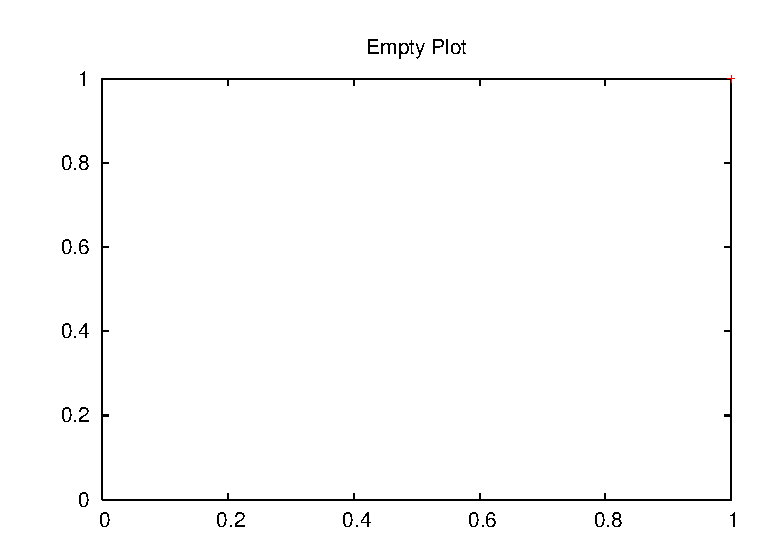
\includegraphics[height=1.4in]{F/empty.eps}
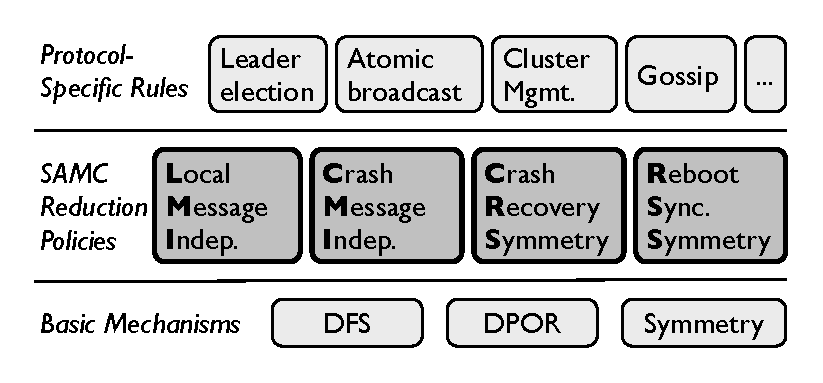
\includegraphics[height=2in]{F/samc/samc.eps}
}
\vminfive
\mycaption[SAMC Architecture]{fig-samc}{SAMC Architecture}{}
%\vminfive
\end{figure}

 % ------ fig samc

% 4 approaches and benefits
Our main contribution lies within our four novel {\em semantic-aware
  reduction policies}: local-message independence (LMI), crash-message
independence (CMI), crash recovery symmetry (CRS), and reboot
synchronization symmetry (RSS).  To the best of our knowledge, none of
these approaches have been introduced in the literature.  At the heart
of these policies are {\em generic event processing patterns} (\ie,
patterns of how messages, crashes, and reboots are processed by
distributed systems).  Our policies and patterns are simple and
powerful; they can be applied to many different distributed systems.  Testers
can extract the patterns from their target protocols (\eg,
leader election, atomic broadcast) and write protocol-specific
rules in few lines of code.

In the next section, we first present our four reduction policies
along with the processing patterns.  Later, we will discuss ways to
extract the patterns from target systems (\sec\ref{sam-extract}) and
then show the protocol-specific rules for our target systems
(\sec\ref{imp-targets}).



\section{Semantic-Aware Reduction Policies}
\label{sam-pol}



We now present four semantic-aware reduction policies that enable us to
define fine-grained event dependency/independency and symmetry beyond
what black-box approaches can do.




% policies

% ------------------------
\subsubsection{Local-Message Independence (LMI)}
\label{sam-lmi}

% LMI basic
We define {\em local messages} as messages that are concurrently in
flight to a given node (\ie, intra-node messages).  As shown in
Figure~\ref{fig-pol}a, a black-box DPOR treats the message processing
semantic inside the node as a black box, and thus must declare the
incoming messages as dependent, leading to 4! permutation
of \ma\mb\mc\md.  On the other hand, with white-box knowledge,
local-message independence (LMI) can define {\em independency
relationship among local messages}.  For example, illustratively in
Figure~\ref{fig-pol}b, given the node's local state (\ls) and the
processing semantic (embedded in the \ts{if} statement), LMI is able
to define that \ma\ and \mb\ are dependent, \mc\ and \md\ are
dependent, but the two groups are independent, which then leads to
only 4 re-orderings.  This reduction illustration is similar to the
one in Section~\ref{mot-state}, but this time LMI enables DPOR
application on local messages.


% LMI question
LMI can be easily added to a dmck.  A dmck server typically has a
complete view of the local states (\sec\ref{mot-bgterms}).  What is
needed is the {\em message processing semantic}: how will a node (\nn)
process an incoming message (\mm) given the node's current local state
(\ls)?  The answer lies in these four simple {\em message processing
patterns} (discard, increment, constant, and modify):


{\small
\begin{alltt}
     \underline{Discard:}           \underline{Increment:}  
     if (pd(m,ls))      if (pi(m,ls))
      (noop);             ls++;       

     \underline{Constant:}          \underline{Modify:}  
     if (pc(m,ls))      if (pm(m,ls))
       ls = Const;        ls = modify(m,ls);
\end{alltt}
}

% LMI pattern .....
In practice, \ls\ and \mm\ contain many fields.  For simplicity, we
treat them as integers.  The functions with prefix \pp\ are boolean
read-only functions (predicates) that compare an incoming message
(\mm) with respect to the local state (\ls); for example, \pd\ can
return true if \ts{m<s}.  The first pattern is a {\em discard} pattern
where the message is simply discarded if \pd\ is true.  This pattern
is prevalent in distributed systems with votes/versions; old
votes/versions tend to be discarded (\eg, our example
in \sec\ref{sam-ex}).  The {\em increment} pattern performs an
increment-by-one update if \pi\ is true, which is also quite common in
many protocols (\eg, counting commit acknowledgements).  The {\em
constant} pattern changes the local state to a constant whenever \pc\
is true.  Finally, the {\em modify} pattern changes the local state
whenever \pm\ is true.


% LMI policy
Based on these patterns, we can  apply LMI in the following
ways.
%
(1) \mx\ is independent of \my\ if \pd\ is true on any of \mx\ and \my.
That is, if \mx\ (or \my) will be discarded, 
then it does not need to be re-ordered 
with other messages.
%
(2) \mx\ is independent of \my\ if \pi\ (or \pc) is true on both \mx\ and \my.
That is, the re-orderings do not matter because the local state is
monotonically increasing by one (or changed to the same constant).
%
(3) \mx\ and \my\ are dependent if \pm\ is true on \mx\ and 
\pd\ is not true on \my.  
That is, since both messages modify the local state in unique ways, then the
re-orderings can be ``interesting'' and hence should be exercised.
%
All these rules are continuously evaluated before every event is
enabled.  If multiple cases are true, dependency has higher precedence
than independency.







% LMI, application 
Overall, LMI allows dmck to smartly skip redundant re-orderings by
leveraging simple patterns.  The job of the tester is to find the
message processing patterns from a target protocol and write {\em
protocol-specific rules} (\ie, filling in the content of the four LMI
predicate functions (\pd, \pi, \pc, and \pm) specific to the target
protocol).  As an example, for our simple leader election protocol
(\sec\ref{sam-ex}), \pd\ can be as simple as:
return \ts{m.vote} \ts{<}
\ts{ls.myVote}.









\begin{figure}[t]

\centerline{
%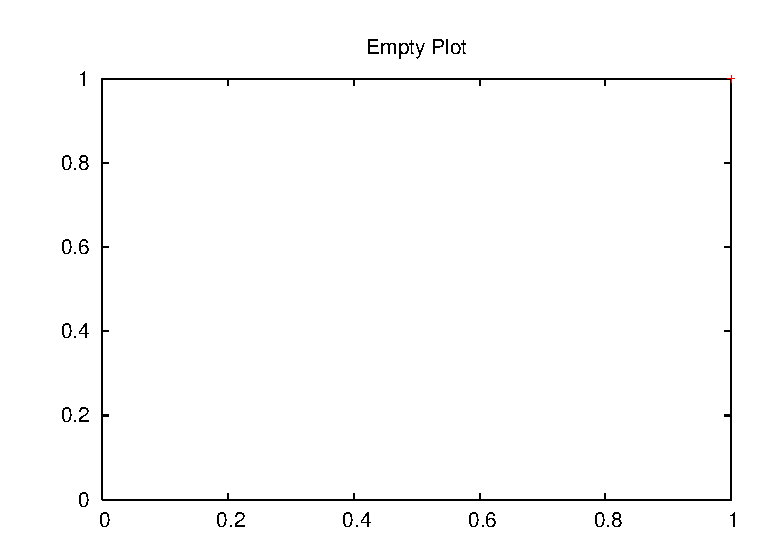
\includegraphics[height=1.2in]{F/empty.eps}
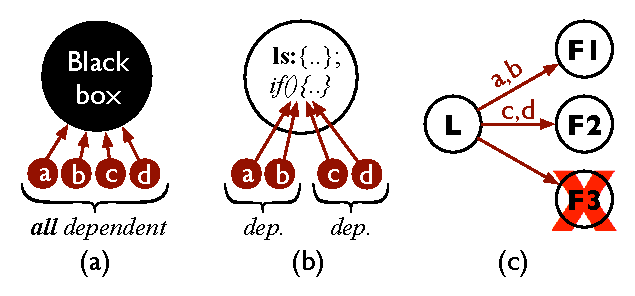
\includegraphics[height=2in]{F/pol/pol.eps}
}
\vminfive
\mycaption[LMI and CMI]{fig-pol}{LMI and CMI}{The figures
illustrate (a) a black-box approach, (b) local-message
independence with white-box knowledge, and (c)
crash-message independence.}
\vminten
\end{figure}





\subsubsection{Crash-Message Independence (CMI)}
\label{sam-cmi}


% CMI motivation
Figure~\ref{fig-pol}c illustrates the motivation behind our next
policy.  The figure resembles an atomic broadcast protocol where a
leader (\ts{L}) sends commit messages to the followers (\ts{F}s).
Let's assume commit messages \ts{ab} to \fone\ and \ts{cd} to \ftwo\
are still in flight (\ie, currently outstanding in the dmck; not
shown).  In addition, the dmck would like to crash \ftri, which we
label as a crash event \xx.  The question we raise is: how should \xx\
be re-ordered with respect to other outstanding messages
(\ma, \mb, \mc, and \md)?


% CMI problem dmck
As we mentioned before, we find {\em no} single dmck that incorporates
crash semantics into reduction policies.  As an implication, in our
example, the dmck must reorder \xx\ with respect to other outstanding
messages, generating executions \ts{Xabcd}, \ts{aXbcd}, \ts{abXcd},
and so on.  Worse, when \ts{abcd} are reordered, \xx\ will be
reordered again.  We find this as one major fundamental problem why
existing dmcks do not scale with the inclusion of failures.

% CMI pattern
To solve this, we introduce crash-message independence (CMI) which
defines {\em independency relationship between a to-be-injected crash
and outstanding messages}.  The key lies in these two crash reaction
patterns (global vs. local impact) running on the surviving nodes
(\eg, the leader node in Figure~\ref{fig-pol}c).


\begin{minipage}{\textwidth}
\begin{alltt}
\vfive
      \underline{Global impact:}       \underline{Local impact:}
      if (pg(X,ls))         if (pl(X,ls)) 
        modify(ls);           modify(ls);
        sendMsg();           
\end{alltt}
\vfive
\end{minipage}


% CMI pattern
The functions with prefix \pp\ are predicate functions that compare
the crash event \xx\ with respect to the surviving node's local state
(\eg, the leader's local state).  The \pg\ predicate in the {\em
global-impact} pattern defines that the crash \xx\ during the local
state \ls\ will lead to a local state change {\em and} new outgoing
messages (\eg, to other surviving nodes).  Here, no reduction can be
done because the new crash-induced outgoing messages must be
re-ordered with the current outstanding messages.  On the other hand,
reduction opportunities exist within the {\em local-impact} pattern,
wherein the \pl\ predicate specifies that the crash will just lead to
a local state change but not new messages, which implies that the
crash does not need to be re-ordered.  


% CMI policies
Based on the two crash impact patterns, we apply CMI in the following ways.
%
Given a local state \ls\ at node \nn, a peer failure \xx, and outstanding
messages (\mone...\mn) from \nn\ to other surviving peers, CMI performs:
%
(1) If \pl\ is true, then \xx\ and \mone...\mn\ are independent.
%
(2) If \pg\ is true, then \xx\ and \mone...\mn\ are dependent.
%
In Figure~\ref{fig-pol}c for example, if \pl\ is true in node \ts{L},
then \xx\ does not impact outstanding messages to \fone\ and \ftwo,
and thus \xx\ is independent to \ts{abcd}; exercising
\ts{Xabcd} is sufficient.


% CMI deployment
An example of CMI application is a quorum-based write protocol.  If a
follower crash occurs and quorum is still established, the leader will
just decrease the number of followers (local state change only).  Here,
for the protocol-specific rules, the tester can specify \pl\ with
\ts{\#follower} \ts{>=} \ts{majority} and \pg\ with the reverse. 
Overall, CMI helps dmck scale with the inclusion of failures, specifically by
skipping redundant re-orderings of crashes with respect to outstanding
messages.





% ---------------------------------
\subsection{Crash Recovery Symmetry (CRS)}
\label{sam-crs}


% RS Extra note
Before we discuss our next reduction policy, we emphasize again the
difference between message event and crash/reboot event.  Message
events are generated by the target system, and thus dmck can only
reduce the number of re-orderings (but it cannot reduce the events).
Contrary, crash events are generated by dmck, and thus there exists
opportunities to reduce the number of injected crashes.  For example,
in Figure~\ref{fig-pol}c, in addition to crashing \ftri, the dmck can
also crash \fone\ and \ftwo\ in different executions, but that might
not be necessary.

\input{code-crash}

% intuition: no individual node Ids, recovery depends on different states
To omit redundant crashes, we develop crash recovery symmetry (CRS).
The intuition is that some crashes often lead to symmetrical recovery
behaviors.  For example, let's assume a 4-node system with node
roles \ts{FFFL}.  At this state, crashing the first or second or third
node perhaps lead to the same recovery since all of them are
followers, and thereby injecting one follower crash could be enough.
Further on, if the system enters a slightly different
state, \ts{FFLF}, crashing any of the followers might give the same
result as above.  However, crashing the leader in the two cases
(\nfour\ in the first case and \ntri\ in the second) should perhaps be
treated differently because the recovery might involve the dead leader
ID.  The goal of CRS is to help dmck with crash decision.


% challenge
The main question in implementing CRS is: how to incorporate crash
recovery semantics into dmck?  Our solution is to compute {\em recovery
abstract global state} (\rags), a simple and concise representation of
crash recovery.  CRS builds \rags\ with the following steps:

First, we define that two recovery actions are symmetrical if they
produce the same messages and change the same local states in the same
way.

Second, we extract recovery logic from the code by flattening the
predicate-recovery pairs (\ie, recovery-related \ts{if} blocks).
Figure~\ref{code-crash} shows a simple example.  Different recovery
actions will be triggered based on which recovery predicate
(\prone, \prtwo, or \prtri) is true.  Each predicate depends on the
local state and the information about the crashing node.  Our key here
is to map each predicate-recovery pair to this formal pattern:


\vmintwo
{\small
\begin{alltt}
    if (\pri(ls, C.ls)) 
       modify(\ralsi); 
       \textit{(and/or)}
       sendMsg(\ralsi);
\end{alltt}
}
\vmintwo

Here, \pri\ is the recovery predicate for the i-th recovery action, and 
\ralsi\ is the recovery abstract local state 
(\ie, a subset of all fields of the local state involved in 
recovery).  That is, each recovery predicate defines what recovery
abstract local state that matters (\ie, \pri$\rightarrow$\{\ralsi\}).  For example, in Figure~\ref{code-crash},
if \prone\ is true, then \ralsone\ only contains the \ts{follower}
variable; if \prtri\ is true, \ralstri\ contains \ts{role}
and \ts{leaderId} variables.

Third, before we crash a node, we check which \pri\ will be true on
each surviving node and then obtain the \ralsi.  Next, we combine
\ralsi\ of all surviving nodes and {\em sort} them into a recovery
abstract global state (\rags);  sorting \rags\ helps us exploit
topological symmetry (\eg,  individual node IDs often do not matter).


Fourth, given a plan to crash a node, the algorithm above 
gives us the \rags\ that represents the corresponding recovery action.
We also maintain a history of \rags\ of previous injected crashes.
If the \rags\ already exists in the history, then the crash is skipped
because it will lead to a symmetrical recovery of the past.


% here here here
To recap with a concrete example, let's go back to the case
of \ts{FFFL} where we plan to enable crash(\none).  Based on the code
in Figure~\ref{code-crash}, the \rags\ is \{*, $\oslash$,
$\oslash$, \ts{\#follower=3}\}; 
* implies the crashing node, 
$\oslash$ means there is no true
predicate at the other two follower nodes, and \ts{\#follower=3} comes
from \ralsone\ of \prone\ of \nfour\ (the leader).  CRS will sort this
and check the history, and assuming no hit, then crash(\none) will be
enabled.  In another execution, SAMC finds that crash(\ntwo)
at \ts{FFFL} will lead to \rags:\{$\oslash$, *,
$\oslash$, \ts{\#follower=3}\}, which after sorting will hit the
history, and hence crash(\ntwo) is skipped.  If the system enters a
different state \ts{FFLF}, no follower crash will be injected, because
the \rags\ will be the same as above.  In terms of leader crash,
crashing the leader in the two cases will be treated differently
because in a leader crash, \prtri\ is true on followers and \prtri\
involves \ts{leaderId} which is different in the two cases.

% ...
In summary, the foundation of CRS is the computation of recovery
abstract global state (\rags) from the crash recovery logic extracted
from the target system via the \pri$\rightarrow$\{\ralsi\} pattern.
We believe this extraction method is simple because CRS does {\em not}
need to know the specifics of crash recovery; CRS just needs to know
what variables are involved in recovery (\ie, the \rals) .







\subsection{Reboot Synchronization Symmetry (RSS)}
\label{sam-rss}


Reboots are also essential to exercise (\sec\ref{mot-deep}), but if not
done carefully, will introduce more scalability problems.  Reboot reduction
policy is needed to help dmck inject reboots ``smartly''.  The intuition
behind reboot synchronization symmetry (RSS) is similar to that of CRS.
When a node reboots, it typically {\em synchronizes} itself with the peers.
However, a reboot will not lead to a new scenario if the current state of
the system is similar to the state when the node crashed.  To implement
RSS, we extract reboot-synchronization predicates and the corresponding
actions.  Since the overall approach is similar to CRS, we omit further
details.


In our experience RSS is extremely powerful.  For example, it allows
us to find deep bugs involving multiple reboots in the ZooKeeper
atomic broadcast (ZAB) protocol.  RSS works efficiently here because
reboots in ZAB are only interesting if the live nodes have seen new
commits (\ie, the dead node falls behind).  In contrast, a black-box
dmck without RSS initiates reboots even when the live nodes are in
similar states as in before the crash, prolonging the discovery of
deep bugs.





%\input{sam-ptop}
%\input{sam-pprio}



\subsection{Pattern Extraction}
\label{sam-extract}


% summary
We have presented four general, simple, and powerful semantic-aware
reduction policies along with the generic event processing patterns.
With this, testers can write protocol-specific rules by extracting the
patterns from their target systems.  
%
Given the patterns described in previous sections, a tester must
perform what we call as ``extraction'' phase.  Here, the tester must
extract the patterns from the target system and write
protocol-specific rules specifically by filling in the predicates and
abstractions as defined in previous sections; in
Section~\ref{imp-targets}, we will show a real extraction result (\ie,
real rules).  Currently, the extraction phase is manual; we leave
automated approaches as a future work (\sec\ref{discuss}).
Nevertheless, we believe manual extraction is bearable for several
reasons.  First, today is the era of
DevOps~\cite{Limoncelli+11-Devops} where developers are testers and
vice versa; testers know the internals of their target systems.  This
is also largely true in cloud system development.  Second, the
processing patterns only cover high-level semantics; testers just fill
in the predicates and abstractions but no more details.  In fact,
simple semantics are enough to significantly help dmck go faster to
deeper states.





\section{Implementation and Integration}
\label{sec-impl}

In this section, we first describe our SAMC prototype, \sampro, which we
built from scratch because existing dmcks are either
proprietary~\cite{Yang+09-Modist} or only work on restricted high-level
languages (\eg, Mace~\cite{Killian+07-LifeDeathMaceMC}).  We will then describe
\sampro\ integration to three widely popular cloud systems,
ZooKeeper~\cite{Hunt+10-ZooKeeperPaper}, Hadoop/Yarn~\cite{Kumar+13-Yarn},
and Cassandra~\cite{Lakshman+09-Cassandra}.  Prior to \sampro, there was no
available dmck for these systems; they are still tested via unit tests, and
the test code size is bigger than the main code, but the tests are far from
reaching deep bugs.






\section{\sampro}
\label{imp-pro}

\sampro\ is written in \numLinesSamPro\ lines of code in Java, which
includes all the components mentioned in Section~\ref{mot-bgterms} and
Figure~\ref{fig-dmck}.  The detailed anatomy of dmck has been
thoroughly explained in literature~\cite{Guerraoui+11-McNoNetwork,
  Guo+11-Demeter, Killian+07-LifeDeathMaceMC, Simsa+10-Dbug,
  Yang+09-Modist}, and therefore for brevity, we will not discuss many
engineering details.  We will focus on SAMC-related parts.

% access source code
We design \sampro\ to be highly portable; we do not modify the target code
base significantly as we leverage a mature interposition technology,
AspectJ, for interposing network messages and timeouts.
% local state
Our interposition layer also sends local state information to the
\sampro\ server.
% crashes and reboots
\sampro\ is also equipped with crash and reboot scripts specific to the
target systems.  The tester can specify a budget of the maximum number of
crashes and reboots to inject per execution.
% summ
\sampro\ employs basic reduction mechanisms and advanced reduction policies
as described before.
% checks
We deploy safety checks at the server (\eg, no two leaders).  If a
check is violated, the trace that led to the bug is reported and 
can be deterministically replayed in \sampro.
% other supports
Overall, we have built all the necessary features to show the case of
SAMC.  Other features such as intra-node thread
interleavings~\cite{Guo+11-Demeter}, scale-out
parallelism~\cite{Simsa+12-ScalablePOR}, and virtual clock for network
delay~\cite{Yang+09-Modist} can be integrated to \sampro\ as well.




\vten % orphan text

\section{Integration to Target Systems}
\label{imp-targets}


In our work, the target systems are ZooKeeper, Hadoop 2.0/Yarn, and
Cassandra.  ZooKeeper~\cite{Hunt+10-ZooKeeperPaper} is a distributed
synchronization service acting as a backbone of many distributed systems
such as HBase and High-Availability HDFS.  Hadoop
2.0/Yarn~\cite{Kumar+13-Yarn} is the current generation of Hadoop that
separates cluster management and processing components.
Cassandra~\cite{Lakshman+09-Cassandra} is a distributed key-value store
derived from Amazon Dynamo~\cite{DeCandia+07-Dynamo}.

In total, we have model checked \numProtocols\ protocols: ZooKeeper
leader election (ZLE) and atomic broadcast (ZAB), Hadoop cluster
management (CM) and speculative execution (SE), and Cassandra
read/write (RW), hinted handoff (HH) and gossiper (GS).  These
protocols are highly asynchronous and thus susceptible to message
re-orderings and failures.

Table~\ref{tab-policies} shows a real sample of protocol-specific
rules that we wrote.  Rules are in general very short; we only wrote
\numLinesRule\ lines/protocol on average.  This shows the simplicity
of SAMC's integration to a wide variety of distributed system protocols.




\begin{sidewaystable*}
\begin{center}
{\small
%---------------------------------
\begin{tabular}{p{1.9in}|p{2in}|p{2.1in}|p{2in}} 


\multicolumn{1}{c|}{{\bf Local-Message}} &
\multicolumn{1}{c|}{{\bf Crash-Message}} &
\multicolumn{1}{c|}{{\bf Crash Recovery}} &
\multicolumn{1}{c}{{\bf Reboot Synchronization}}
\\

\multicolumn{1}{c|}{{\bf Independence (LMI)}} &
\multicolumn{1}{c|}{{\bf Independence (CMI)}} &
\multicolumn{1}{c|}{{\bf Symmetry (CRS)}} &
\multicolumn{1}{c}{{\bf Symmetry (RSS)}}
\\


\hline  % =====================================================

% ----------------------------------------------- ZLE, LMI (1)

\vminten
{\footnotesize
\begin{alltt}
bool pd : !newVote(m, s);

bool pm : newVote(m, s);

bool newVote(m, s) : {
 if (m.ep > s.ep) 
   return true; 
 else if (m.ep == s.ep)
  if (m.tx > s.tx) 
   return true;
  else if (m.tx == s.tx &&
           m.lid > s.lid) 
   return true;
}
\end{alltt}
}

& % ----------------------------------------------- ZLE, CMI (1)

\vminten
{\footnotesize
\begin{alltt}
bool pg (s, X) : 
 if (s.rl == F && X.rl == L)
  return true;
 if (s.rl == L && X.rl == F
     && !quorumAfterX(s)
  return true;
 if (s.rl == S && X.rl == S) 
  return true;

bool pl (s, X) :
 if (s.rl == L && X.rl == F 
     && quorumAfterX(s)) 
  return true;

bool quorumAfterX(s) :
  ret ((s.fol-1) >= 
        s.all/2);
\end{alltt}
}

& % ----------------------------------------------- ZLE, CRS (1)

\vminten
{\footnotesize
\begin{alltt}
bool pr1(s,C):
 if (s.rl == L && C.rl == F
     && quorumAfterX(s))
  return true;
rals1:\{rl,fol,all\};

bool pr2(s,C):
 if (s.rl == L && C.rl == F 
     && !quorumAfterX(s))
 return true;
rals2: \{rl,fol,lid,ep,tx,clk\}

bool pr3(s,C):
 if (s.rl == F && c.rl == L)
  return true;
rals3: \{rl,fol,lid,ep,tx,clk\}

bool pr4:
 if (s.rl == S)
  return true;
rals4: \{rl,lid,ep,tx,clk\}
\end{alltt}
}


& % ----------------------------------------------- ZLE, RSS (1)

\vminten
{\footnotesize
\begin{alltt}
bool ps1(s,R):
 if (s.rl == L)
  return true;
sals1: \{rl,lid,ep,tx,clk\}

bool ps2(s,R):
 if (s.rl == F)
  return true;
sals2: \{rl,lid,ep,tx,clk\}

bool ps3(s,R):
 if (s.rl == S && 
     s.clk > R.clk)
  return true;
sals3: \{rl,lid,ep,tx,clk\}

bool ps4(s,R):
 if (s.rl == S && 
     moreUpdated(s, R))
  return true;
sals4: \{rl,lid,ep,tx,clk\}

bool moreUpdated(s, R):
 if (R.ep > s.ep)
  return true;
 else if (R.ep == s.ep)
  if (R.tx > s.tx) 
   return true;
  else if (R.tx == s.tx)
   if (R.lid > s.lid)
    return true;
\end{alltt}
}

\end{tabular}
}
%---------------------------------
\end{center}
%
\vminfive
\mycaption[Protocol-Specific Reduction Rules for ZLE]{tab-policies}{Protocol-Specific Reduction Rules for ZLE}{
%
The code above shows the actual protocol-specific rules for
ZLE protocol.  These rules are the inputs to the four reduction policies.
%
Many variables are abbreviated (ep: epoch, tx: latest
transaction ID, lid: leader ID, rl: role, fol: follower count, all: total
node count, clk: logical clock, L: leading, F: following, S: searching,
X/C: crashing node, R: rebooting node). LMI \pc\ and \pi\ predicates are not 
used for ZLE, but used for other protocols. 
%
}
%\vminfive
\end{sidewaystable*}


\if 0
zle-specific rule = 49
zab-specific rule = 33
mapreduce: 35 ..
protocol average = 
\fi




\section{Evaluation}

\subsection{Result}

We have built SAMC from scratch, and it took around 10,000 lines of code for all
mechanism.

We integrated to 7 protocols on 3 cloud systems, ZooKeeper, Cassandra,
MapReduce, including 10 version, new and old.

\subsection{Protocol-Specific Rules}

This is an example of protocol-specific rules from ZooKeeper leader election.

On average, it takes 35 lines of code for each protocols.

\subsection{Catching Old Bugs}

We can re-produce 12 old bugs that were reported by running SAMC with old
version of cloud systems.

We compare it with other state-of-the-art techniques, black-box DPOR that is
DPOR without domain-specific knowledge, random that is randomly re-ordering the
events, and random DPOR that is DPOR that start with random ordering.

Then we measure how many executions each model checker has to run until it reach
bugs.

By execution, I mean the ordering of events since the beginning up to
termination point or seeing some bugs.

This is SAMC.

This is black-box DPOR. This is random.

This is random DPOR.

5000+ means we have run 5000 executions but still not catch the bugs, and that
was around 2 days.

And here we compute speed-up.

Compare to black box, SAMC can do more than 94 times faster

And about 300 times faster compare to random and random DPOR.

\subsection{Reduction Ratio}

We also calculated reduction ratio compare to black- box DPOR on ZooKeeper
leader election protocol.

We also did fine-grained evaluation for each reduction policy too.

By trying different crashes and reboot, the result is shown in this table.

The reduction ratio increases when the number of crash and reboot increases. And
that means SAMC can find deep bugs faster than other techniques.

\subsection{Conclusion}

Today, we have cloud systems that quite complex, and deep bugs do happen to the
systems.

One approach to catch deep bugs is distributed system model checker, however,
the model checker treats the system as a black box and lead to state space
explosion

We are showing here that if we open the black box, make understanding of the
semantic, we can detect unnecessary ordering that lead to the same state, we
remove that and get one to two order of magnitude speedup

I believe that in the future we can use the principal of semantic awareness to
build more efficient reduction policies.



\chapter{A Case of Scalability Bug in Cloud-Scale Distributed Systems}
\label{chp-scb}

In this and next chapter, we will focus on scalability aspect of cloud backend.
As we mention in Section \ref{bg-sc}, the trend goes to horizontal scaling or
scale-out systems, and this introduces a new class of bugs that does not exist
in single-machine software or small-scale distributed systems, which we call
these bugs ``scalability bugs''. 
%
%Becuase these bugs are new, there have been few efforts pay attention to them.
There are a lot of efforts that try to improve scalability of different parts of
distributed systems \cite{Boutin+14-Apollo, Ousterhout+13-Sparrow,
Ganjam+15-C3Video, Glendenning+11-Scatter, Lloyd+11-COPS}, but we find little
work focusing on testing scalability of the systems \cite{Gupta+08-DieCast,
Wang+14-Exalt} so this is still an open problem.

The naive way to test system scalability is deploying systems on an actual large
cluster, however, doing so is very expensive and not all developers have access
to such luxurious resources (\eg, voluntary open-source developers). To
introduce an economical testing approach, we need more insights about these
bugs, yet we find no work performs study or analysis to understand them
in-detail. Thus, like the way we tackle DC bugs, we start our research on
combating scalability bugs by performing a study on them first. We study
\totAll scalability bugs from different popular scalable distributed systems. 
%
This chapter shows our observations from the study that will highlights an
urgency in tackling scalability bugs. Section \ref{sec-scb-mot} discusses
motivation in tackling scalability bugs and show an example of real a
scalability bug in Cassandra, and Section \ref{mot-observe} gives the
observations we gain from the study.
%
%This chapter highlights an urgency in tackling scalability bugs by studying
%deeply in \totAll scalability bugs from different popular scalable distributed
%systems. Section \ref{sec-scb-mot} discusses motivation in tackling
%scalability bugs and Section \ref{mot-observe} gives some observations we gain
%from the study.

\section{Motivation}
\label{sec-scb-mot}

% scale, scale ... 
Is scale a friend or a foe \cite{Ousterhout+11-ScaleFriendEnemy}?
% CACM, is scale friend or enemy, john ousterhout
On the positive side, scale surpasses the limit of a single machine in
meeting users' increasing demands of compute and storage, which led to
many inventions of ``cloud-scale'' distributed systems
\cite{Chang+06-BigTable, 
DeanGhemawat04-MapReduce, 
DeCandia+07-Dynamo,
Ghemawat+03-GoogleFS, 
Hindman+11-Mesos,
Verma+15-Borg}.  The field has witnessed a
phenomenal deployment scale of such systems;
%
Netflix runs tens of 500-node Cassandra clusters \cite{RunningNetflix13},
% Running Netflix on Cassandra in the Cloud (youtube), Adriak Crockcroft
% https://www.youtube.com/watch?v=97VBdgIgcCU
Apple deploys a total of 100,000 Cassandra nodes \cite{WikiCassandra}, 
% https://en.wikipedia.org/wiki/Apache_Cassandra
and Yahoo! recently revealed the use of 40,000 Hadoop servers,
with a 4500-node cluster as the largest one \cite{LargestHadoop}.
% Http://www.techrepublic.com/article/why-the-worlds-largest-hadoop-installation-may-soon-become-the-norm/

% dark side, foe
On the negative side, scale creates new development and deployment issues.
Developers must ensure that their algorithms and protocol designs
to be scalable.
However, until real deployment takes place, scalability bugs 
in the actual implementations are unforeseen.
% more and more
These scalability bugs are latent bugs that
are scale-dependent; they only surface in large-scale deployments, but not
in small/medium-scale ones. Their presence jeopardizes systems
reliability and availability at scale.

As an example, let us consider a bug in Cassandra, a highly-scalable
peer-to-peer key-value store.  If a user initially deploys a cluster of 50 nodes
and later scales it out with 50 additional nodes, the operation can be done
smoothly. However, if the user deploys a 200-node cluster and then adds 200
more nodes, the protocol that rebalances the key-range partitions (which nodes
should own which key ranges) becomes CPU intensive as the calculation has an
$O(N^3)$ complexity where $N$ is the number of nodes.  This combined with the
gossiping and failure detection logic leads to a scalability bug that makes the
cluster unstable (many live nodes are declared as dead, making some data not
reachable by the users). We give full detail of the Cassandra bug in Section
\ref{mot-bug}.

% example
We perform an in-depth study of
\totAll scalability bugs reported from the deployments
of popular large-scale systems such as
Hadoop,
HBase,
HDFS,
Cassandra,
Couchbase,
Riak, and
Voldemort.
%
From this study, we observed many challenges in finding, reproducing, and
debugging scalability bugs.
%
As in the example above, bug symptoms sometimes surface only in large
deployment scales (\eg, $N$$>$100 nodes), hence small/medium-scale testing
is not enough.  Yet, not all developers have large test budgets, and even
when they do, debugging on hundreds of nodes is time consuming and
difficult.
%
Furthermore, protocol algorithms can be scalable in the design sketches,
but not necessarily in the real deployments; there are specific
implementation details whose implications at scale are hard to predict. We
discuss more about our observations on scalability bugs in Section \ref{mot-observe}.



\subsection{A Sample Cassandra Bug}
\label{mot-bug}

\begin{figure}

\centerline{
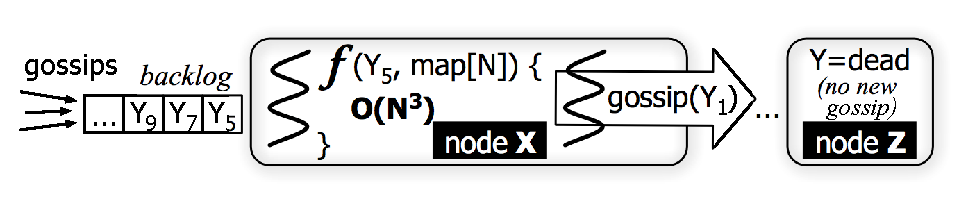
\includegraphics[height=0.8in]{F/cass1.eps}
%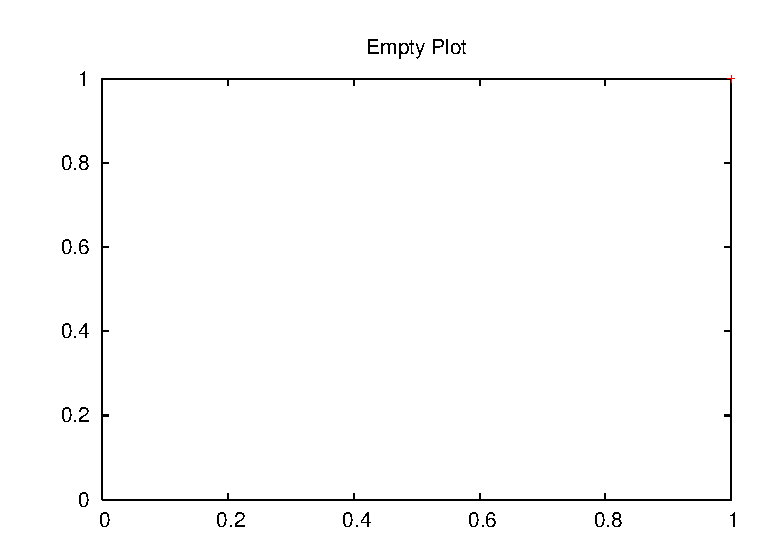
\includegraphics[height=0.6in]{F/empty.eps}
}
\vminfive
\mycaption{fig-cass1}{The problem of
gossip-based failure detection in Cassandra}{}
\vminfive
\end{figure}



We now describe in detail a scalability bug in Cassandra, which we use as a
sample bug.
%
Our journey in understanding scalability bugs began when we observed repeated
``flapping'' problems in large-scale Cassandra deployments (\ie, hundreds of
nodes).
%
Flapping is a cluster instability problem where node's up/down status
continuously flaps.  A ``flap'' is when a node X marks a peer node Y as down
(and soon marks Y as alive again).
%
We rigorously study a series of Cassandra bugs below that surfaced as the code
evolved.

%
%The bug surfaced on a cluster with hundreds of nodes and led to
%``\textit{\textbf{flapping}}'' nodes, a condition where node up/down status
%continuously changes;  tens of thousands of flaps\footnote{A ``\textbf{flap}''
%is when a node X marks a peer node Y as down.}  were observed.

To understand this bug, we need to understand the following protocols.

\begin{enumerate}

\item {\bf Bootstrap:} Each node first creates partition keys (\eg, 32 random
numbers) and gossips this information to peer nodes.
 
\item {\bf Gossip broadcast:} {\em Every second}, each node gossips to one
random node about a list of nodes and partitions it knows (including itself)
and their {\em version} numbers.  Each node also increments its version number
(``I'm still alive'') before gossiping.
 
\item {\bf Gossip processing:} The receiving node then finds any state
(metadata) differences between the two nodes to synchronize their views of the
ring.  Eventually, all nodes know about each other.
 
\item {\bf Failure detection:} {\em Every second}, a failure detection daemon
runs \cite{Lakshman+09-Cassandra}.  Put simply, if a node X has not received a
new gossip about Y {\em from anyone} (Y's version has not changed after some
period of time), X will declare Y dead (a flap).  When X receives a new gossip
about Y, it marks Y alive.

\end{enumerate}

% about the bug
There are two factors that induce the bug. The first is the {\em long latency
of scale-dependent state-update gossip processing during bootstrapping} (``f''
in Figure \ref{fig-cass1}).  While gossip processing is usually fast in a
stable cluster, it is expensive during bootstrapping as the gossips carry many
new state changes about the ring; the state-update processing time is
scale-dependent (\ie, greater than $O(N^3)$); the larger the cluster ($N$), the
larger the ring map, the longer the processing time is.
%
This long latency is caused by {\bf (1)} state-update checkpoint to on-disk
database and {\bf (2)} multi-map cloning and updates.
%
The first one is needed for fast fault tolerance; after a node crashes, it can
reboot fast as it knows the latest view of the ring.
%
The second one is preferred for simplicity; Cassandra clones its \ts{MultiMap}
ring table and applies changes one by one to alleviate long write locks.
%
% in order to prevent a long write lock on the ring table which can block other
% user-facing protocols.

% long
The second factor is the {\em single threaded} implementation of gossip
processing. As shown in Figure \ref{fig-cass1},  this inability to process
multiple gossips/state updates concurrently (for the sake of preventing
concurrency bugs) creates a {\em backlog} of new gossips.  For example, in {\em
every second}, Y tells someone it's alive with increasing version number (\eg,
Y$_7$), but the receiving nodes are still busy processing state changes and
only forward Y's old version number (\eg, Y$_1$).  As Y's new gossip is not
propagated on time,  other nodes (\eg, Z) will mark Y as dead.  This happens to
all nodes, not just Y.

% \ca{3831} -------------------------------------------------
The journey starts with Bug \#\ca{3831} \cite{CA-Two}, when a node D is
decommissioned from a cluster ring, D initiates a gossip telling that all other
nodes must rebalance the ring's key-ranges.  This scale-dependent ``pending
key-range calculation'' is CPU intensive with
%
% $O((n^2)log(n))$   % OLD
$O(MN^3log^3(N))$  % Tanakorn
%
complexity; $M$~is the list of key-range changes in the gossip message.  This
in turn leaves many gossips not propagated on time, creating flapping symptoms
that only appear at scale (at 200+ nodes; \sec\ref{sec-eval}). The developers
then optimized the code to
%
% $O(nlog(n))$  % OLD
$O(MN^2log^2(N))$ complexity.



% \ca{3881} -------------------------------------------------
Soon afterwards (Bug \#\ca{3881} \cite{CA-Tri}), Cassandra added the concept of
virtual partitions/nodes (\eg, $P$$=$$256$ per physical node).  As an
implication, the fix above did not scale as ``$N$'' becomes $N$$\times$$P$.
%
The bug was fixed with a complete redesign of the pending key-range
calculation, making it
% $O(log(N))$ OLD
$O(MNPlog^2(NP))$.

% \ca{5456} -------------------------------------------------
About a year later (\ca{5456} \cite{CA-Four}), Cassandra code employs
multi-threading between the pending key-range calculation and the gossip
processing with a coarse-grained lock to protect sharing of the ring
table.  Unbeknownst to the developers, at scale, the key-range calculation
can acquire the lock for a long time, causing flapping to reappear again.
The fix clones the ring table for the key-range calculation, to release the
lock early.



% \ca{6127} -------------------------------------------------
Later on (\ca{6127} \cite{CA-One}), a similar bug reappeared.  In the above
cases, the problems appeared when the cluster grows/shrinks gradually.
However, if user bootstrap a large cluster (\eg, 500+ nodes) from
scratch (\ie, all nodes do not know each other, with no established
key ranges),
%
the execution traverses a different code path that
performs a fresh ring-table/key-range construction with
$O(MN^2)$ % KORN
complexity.

% \tl{and there is no existing data stored in   the cluster}), 
% \tl{the offending function becomes the keyrange construction} 
%
% keyrange calculation which clones the ring table (a
% \ts{MultiMap}) becomes very expensive.  
%
% Including the cloning $O(N*P)$, we observed an 
% $O(N^3)$  $O(MN^2)$ % KORN complexity.

% ...............
The story continues on (\ca{6345}, \ca{6409}, \etc).  Fast forward today,
Cassandra developers recently started a new umbrella ticket for discussing
``Gossip 2.0,''  supposedly scalable to 1000+
nodes \cite{Gossip20, Gossip20Mail}.
% ---- 
Similar to Cassandra, other large-scale systems are prone to the same
problem.  So far, we have collected and analyzed \totCass Cassandra, \totCouch
Couchbase, \totHadoop Hadoop, \totHBase HBase, \totHDFS HDFS, \totRiak
Riak, and \totVold Voldemort scalability bugs, all caused user-visible
impacts.
%
This manual mining was arduous because there is no searchable jargon for
``scalability bugs''; we might have missed other bugs.
%



\section{Observations}
\label{mot-observe}

From the bug in previous section and all the bugs we studied, we make several
important observations.
%  regarding control-plane scalability bugs and distributed system designs.

\begin{itemize}
% only appear in large scale .. 
\item {\em Only appear at extreme scale:} \caone does not surface in 30-node
deployment.  In 128-node cluster, the symptom appears mildly (tens of
flaps).  From 200-500 nodes, flapping skyrockets from hundreds to 
thousands of flaps.  Testing in small/medium scales is not sufficient,
which is also true for other bugs we studied (\sec\ref{sec-eval}).





% theory is not enough
\item {\em Scalable in design, but not in practice.}  Related to \caone,
the accrual failure detector/gossiper
\cite{Hayashibara+04-PhiFailureDetector} was interestingly adopted by
Cassandra as it is scalable in design \cite{Lakshman+09-Cassandra}.
However, the design proof does not account gossip processing time during
bootstrap, which can be long.  To understand the bug, the developers tried
to ``do the [simple] math'' \cite{CA-One} but failed.  In practice, the
assumption that new gossips are propagated every second is not met (due to
the backlog).  The actual implementations overload gossips with many other
purposes (\eg, announcing boot/rebalance changes) beyond their original
design sketch.



% deep
\item {\em Implementation specific and hard to predict.}  The
backlog-induced flapping in \caone was caused specifically by Cassandra's
implementation choice: metadata checkpoint, multi-map cloning, and its
single-threaded implementation.  State-update processing time is hard to
predict (ranges from 0.001 to 4 seconds) as it depends on a 2-dimensional
input: the receiving node's ring table size and the number of new
state changes (\sec\ref{sec-eval}).

% a two-dimensional input; more in \sec\ref{sec-eval}).  

% not independent
\item {\em Cascading impacts of ``not-so-independent'' nodes.}  In 
cluster-wide control protocols, distributed nodes are  not
necessarily independent; nodes must communicate with each other
to synchronize their views of cluster metadata.  As the cluster grows, the
cluster metadata size increases.  Thus, unpredictable processing time in
individual nodes can create cascading impacts to the whole cluster.


% 
\item {\em Long and difficult large-scale debugging:} 
%
The bug report of \caone generated over 40 back-and-forth discussion
comments and took 2 months to fix.  It is apparent \cite{CA-One} that
there were many hurdles of deploying and debugging the buggy protocol at
real scale.  Important to note is that debugging is {\em not} a single
iteration; developers must {\em repeatedly} instrument the system (add
more logs) and re-run the system at scale to find and fix the bug, which
is not trivial.  The scalability bugs we studied took 6 to 157 days to
fix (27 on average).


\item {\em Not all developers have large test budgets:}
%
Another factor of delayed fixes is the lack of budget for large
test clusters.  Such luxury tends to be accessible to developers 
in large companies, but not to 
open-source developers.  When
\caone was submitted by a customer who had hundreds of nodes, the
Cassandra developers did not have an instant access to a test cluster of
the same scale.



% repeated 
\item {\em Quick fixes and repeated bugs:} Bugs are often fixed with quick
patches (development pressures), but the new fix might not eradicate the
problem completely \cite{Yin+11-FixesBecomeBugs}.
%
For example, for \caone, the patch simply disables failure detection during
bootstrap.  As the protocol was not redesigned, the bug still appeared in
another workload (\eg, scaling out from 128 to 256 nodes).
%
In the latest Cassandra, the simple fix has been removed and the gossip
protocol has been redesigned.
%
We also found that old fixes can become obsolete in 
protocol re-designs, which then can give birth to new scalability bugs. 
%
For example, the fix for \ca{3831} became obsolete as ``vnodes'' was
introduced, which then gave rise to a new 
vnode-related scalability bug
(\ca{3881}).
%
A scale-check could have ensured that new fixes remove old scalability bugs
entirely and similar bugs do not re-surface in new designs.
\end{itemize}


\if 0
Our observations above accentuate the need for scale-checking distributed
system {\em implementations} at {\em real scale}, not via simulation nor
extrapolation.  In this context, we now discuss the state of the art.
\fi


\section{Conclusion}


\chapter{\sck: A Single-Machine Approach for Finding Scalability Bugs in Cloud-Scale Distributed Systems}
\label{chp-sck}


In the previous two chapters, we discuss about distributed concurrency bugs
that how we make sense of them and how we advance the state of the art of model
checking to unearth them faster. In this chapter, we will focus on
scalability aspect of cloud backend. As we mention in Section \ref{bg-sc}, the
trend of cloud distributed systems goes to horizontal scaling or scale-out systems.
On the positive side, scale surpasses the limit of a single machine in
meeting users' increasing demands of computing and storage, which led to
many inventions of ``cloud-scale'' distributed systems
\cite{Chang+06-BigTable, 
DeanGhemawat04-MapReduce, 
DeCandia+07-Dynamo,
Ghemawat+03-GoogleFS, 
Hindman+11-Mesos,
Verma+15-Borg}. The field has witnessed a
phenomenal deployment scale of such systems;
%
Netflix runs tens of 500-node Cassandra clusters \cite{RunningNetflix13},
% Running Netflix on Cassandra in the Cloud (youtube), Adriak Crockcroft
% https://www.youtube.com/watch?v=97VBdgIgcCU
Apple deploys a total of 100,000 Cassandra nodes \cite{WikiCassandra}, 
% https://en.wikipedia.org/wiki/Apache_Cassandra
and Yahoo! recently revealed the use of 40,000 Hadoop servers,
with a 4500-node cluster as the largest one \cite{LargestHadoop}.
% Http://www.techrepublic.com/article/why-the-worlds-largest-hadoop-installation-may-soon-become-the-norm/

% dark side, foe
On the negative side, scale creates new development and deployment issues.
Developers must ensure that their algorithms and protocol designs to be
scalable.  However, until real deployment takes place, scalability bugs in the
actual implementations are unforeseen.
% more and more
These scalability bugs are latent bugs that are scale-dependent; they only
surface in large-scale deployments, but not in small/medium-scale ones. Their
presence jeopardizes systems reliability and availability at scale.

In this chapter, we show our observations from our initial study on scalability
bugs that highlights an urgency in tackling scalability bugs and our pilot work
to introduce a single-machine testing methodology to check scalability of the
systems. Section \ref{sec-sck-observe} discusses about our initial study and shows our
observations toward scalability bugs; Section \ref{mot-state} discusses about the state
of the art; Section \ref{sec-sck-sck}-\ref{sec-sck-eval} explains our pilot work on scalability
bug checking named \sck and some evaluations.


\section{Scalability Bug}
\label{sec-sck-observe}

% example
To begin our work on combating scalability bugs, we start by conducting a study
to see their nature and how critical they are.
%
We perform a study of
\totAll scalability bugs reported from the deployments
of popular large-scale systems such as
Hadoop,
HBase,
HDFS,
Cassandra,
Couchbase,
Riak, and
Voldemort.
%
From the study, we observed many challenges in finding, reproducing, and
debugging scalability bugs. For example, let us consider a bug in Cassandra, a
highly-scalable peer-to-peer key-value store. If a user decommissions a single
node from a cluster of 50 nodes, the operation can be done smoothly. However, if
the user decommissions a node from a cluster of 200 nodes, the protocol that
re-calculate the key-range partitions (which nodes should own which key ranges)
becomes CPU intensive as the calculation has an $O(N^3)$ complexity where $N$ is
the number of nodes.  This combined with the gossiping and failure detection
logic leads to a scalability bug that makes the cluster unstable (many live
nodes are declared as dead, making some data not reachable by the users). We
give a full detail of the Cassandra bug in Section \ref{mot-bug}.

%
As in the example above, bug symptoms sometimes surface only in large deployment
scales (\eg, $N$$>$100 nodes), hence small/medium-scale testing is not enough.
Yet, not all developers have large test budgets, and even when they do,
debugging on hundreds of nodes is time consuming and difficult.
%
Furthermore, protocol algorithms can be scalable in the design sketches, but not
necessarily in the real deployments; there are specific implementation details
whose implications at scale are hard to predict. We discuss more about our
observations on scalability bugs in Section \ref{mot-observe}.

\subsection{A Sample Cassandra Bug}
\label{mot-bug}

\begin{figure}

\centerline{
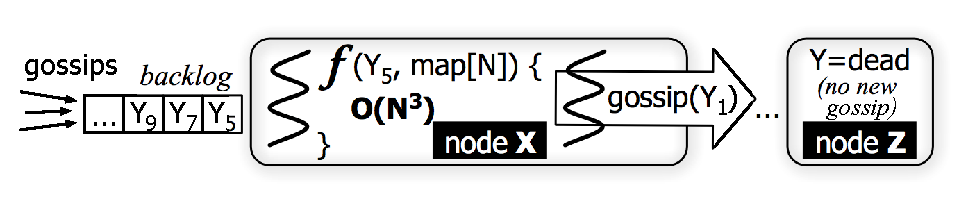
\includegraphics[height=0.8in]{F/cass1.eps}
%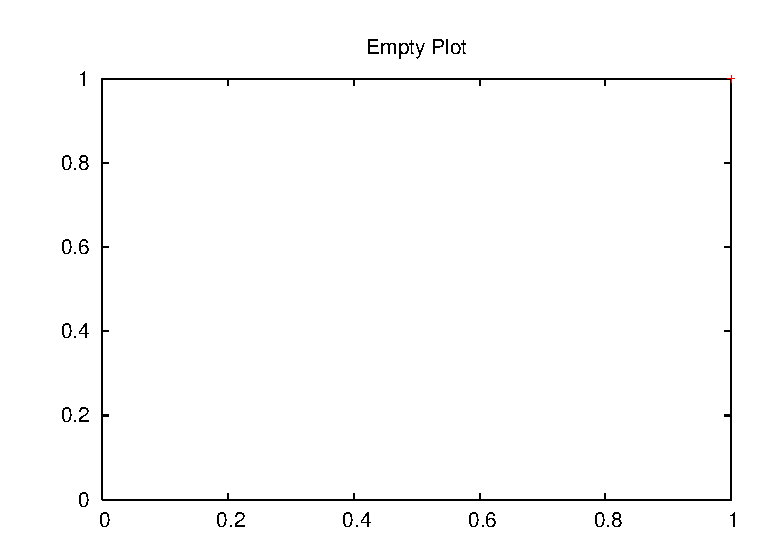
\includegraphics[height=0.6in]{F/empty.eps}
}
\vminfive
\mycaption{fig-cass1}{The problem of
gossip-based failure detection in Cassandra}{}
\vminfive
\end{figure}



We now describe in detail a scalability bug in Cassandra, which we use as a
sample bug.
%
Our journey in understanding scalability bugs began when we observed repeated
``flapping'' problems in large-scale Cassandra deployments (\ie, hundreds of
nodes).
%
Flapping is a cluster instability problem where node's up/down status
continuously flaps.  A ``flap'' is when a node X marks a peer node Y as down
(and soon marks Y as alive again).
%
We rigorously study a series of Cassandra bugs below that surfaced as the code
evolved.

%
%The bug surfaced on a cluster with hundreds of nodes and led to
%``\textit{\textbf{flapping}}'' nodes, a condition where node up/down status
%continuously changes;  tens of thousands of flaps\footnote{A ``\textbf{flap}''
%is when a node X marks a peer node Y as down.}  were observed.

To understand this bug, we need to understand the following protocols.

\begin{enumerate}

\item {\bf Bootstrap:} Each node first creates partition keys (\eg, 32 random
numbers) and gossips this information to peer nodes.
 
\item {\bf Gossip broadcast:} {\em Every second}, each node gossips to one
random node about a list of nodes and partitions it knows (including itself)
and their {\em version} numbers.  Each node also increments its version number
(``I'm still alive'') before gossiping.
 
\item {\bf Gossip processing:} The receiving node then finds any state
(metadata) differences between the two nodes to synchronize their views of the
ring.  Eventually, all nodes know about each other.
 
\item {\bf Failure detection:} {\em Every second}, a failure detection daemon
runs \cite{Lakshman+09-Cassandra}.  Put simply, if a node X has not received a
new gossip about Y {\em from anyone} (Y's version has not changed after some
period of time), X will declare Y dead (a flap).  When X receives a new gossip
about Y, it marks Y alive.

\end{enumerate}

% about the bug
There are two factors that induce the bug. The first is the {\em long latency
of scale-dependent state-update gossip processing during bootstrapping} (``f''
in Figure \ref{fig-cass1}).  While gossip processing is usually fast in a
stable cluster, it is expensive during bootstrapping as the gossips carry many
new state changes about the ring; the state-update processing time is
scale-dependent (\ie, greater than $O(N^3)$); the larger the cluster ($N$), the
larger the ring map, the longer the processing time is.
%
This long latency is caused by {\bf (1)} state-update checkpoint to on-disk
database and {\bf (2)} multi-map cloning and updates.
%
The first one is needed for fast fault tolerance; after a node crashes, it can
reboot fast as it knows the latest view of the ring.
%
The second one is preferred for simplicity; Cassandra clones its \ts{MultiMap}
ring table and applies changes one by one to alleviate long write locks.
%
% in order to prevent a long write lock on the ring table which can block other
% user-facing protocols.

% long
The second factor is the {\em single threaded} implementation of gossip
processing. As shown in Figure \ref{fig-cass1},  this inability to process
multiple gossips/state updates concurrently (for the sake of preventing
concurrency bugs) creates a {\em backlog} of new gossips.  For example, in {\em
every second}, Y tells someone it's alive with increasing version number (\eg,
Y$_7$), but the receiving nodes are still busy processing state changes and
only forward Y's old version number (\eg, Y$_1$).  As Y's new gossip is not
propagated on time,  other nodes (\eg, Z) will mark Y as dead.  This happens to
all nodes, not just Y.

% \ca{3831} -------------------------------------------------
The journey starts with Bug \#\ca{3831} \cite{CA-Two}, when a node D is
decommissioned from a cluster ring, D initiates a gossip telling that all other
nodes must rebalance the ring's key-ranges.  This scale-dependent ``pending
key-range calculation'' is CPU intensive with
%
% $O((n^2)log(n))$   % OLD
$O(MN^3log^3(N))$  % Tanakorn
%
complexity; $M$~is the list of key-range changes in the gossip message.  This
in turn leaves many gossips not propagated on time, creating flapping symptoms
that only appear at scale (at 200+ nodes). The developers
then optimized the code to
%
% $O(nlog(n))$  % OLD
$O(MN^2log^2(N))$ complexity.



% \ca{3881} -------------------------------------------------
Soon afterwards (Bug \#\ca{3881} \cite{CA-Tri}), Cassandra added the concept of
virtual partitions/nodes (\eg, $P$$=$$256$ per physical node).  As an
implication, the fix above did not scale as ``$N$'' becomes $N$$\times$$P$.
%
The bug was fixed with a complete redesign of the pending key-range
calculation, making it
% $O(log(N))$ OLD
$O(MNPlog^2(NP))$.

% \ca{5456} -------------------------------------------------
About a year later (\ca{5456} \cite{CA-Four}), Cassandra code employs
multi-threading between the pending key-range calculation and the gossip
processing with a coarse-grained lock to protect sharing of the ring
table.  Unbeknownst to the developers, at scale, the key-range calculation
can acquire the lock for a long time, causing flapping to reappear again.
The fix clones the ring table for the key-range calculation, to release the
lock early.



% \ca{6127} -------------------------------------------------
Later on (\ca{6127} \cite{CA-One}), a similar bug reappeared.  In the above
cases, the problems appeared when the cluster grows/shrinks gradually.
However, if user bootstrap a large cluster (\eg, 500+ nodes) from
scratch (\ie, all nodes do not know each other, with no established
key ranges),
%
the execution traverses a different code path that
performs a fresh ring-table/key-range construction with
$O(MN^2)$ % KORN
complexity.

% \tl{and there is no existing data stored in   the cluster}), 
% \tl{the offending function becomes the keyrange construction} 
%
% keyrange calculation which clones the ring table (a
% \ts{MultiMap}) becomes very expensive.  
%
% Including the cloning $O(N*P)$, we observed an 
% $O(N^3)$  $O(MN^2)$ % KORN complexity.

% ...............
The story continues on (\ca{6345}, \ca{6409}, \etc).  Fast forward today,
Cassandra developers recently started a new umbrella ticket for discussing
``Gossip 2.0,''  supposedly scalable to 1000+
nodes \cite{Gossip20, Gossip20Mail}.
% ---- 
Similar to Cassandra, other large-scale systems are prone to the same
problem.  So far, we have collected and analyzed \totCass Cassandra, \totCouch
Couchbase, \totHadoop Hadoop, \totHBase HBase, \totHDFS HDFS, \totRiak
Riak, and \totVold Voldemort scalability bugs, all caused user-visible
impacts.
%
This manual mining was arduous because there is no searchable jargon for
``scalability bugs''; we might have missed other bugs.
%

\subsection{Observations}
\label{mot-observe}

From all the bugs we studied, we make several important observations.
%  regarding control-plane scalability bugs and distributed system designs.

\begin{itemize}
% only appear in large scale .. 
\item {\em Only appear at extreme scale:} This Cassandra bug does not surface
in 30-node deployment.  In 128-node cluster, the symptom appears mildly (tens
of flaps). From 200-500 nodes, flapping skyrockets from hundreds to thousands
of flaps. Testing in small/medium scales is not sufficient, which is also true
for other bugs we studied.

% theory is not enough
\item {\em Scalable in design, but not in practice.}  Related to the Cassandra
bug, the accrual failure detector/gossiper
\cite{Hayashibara+04-PhiFailureDetector} was interestingly adopted by Cassandra
as it is scalable in design \cite{Lakshman+09-Cassandra}.  However, the design
proof does not account gossip processing time during bootstrap, which can be
long.  To understand the bug, the developers tried to ``do the [simple] math''
\cite{CA-One} but failed.  In practice, the assumption that new gossips are
propagated every second is not met (due to the backlog).  The actual
implementations overload gossips with many other purposes (\eg, announcing
boot/rebalance changes) beyond their original design sketch.

% deep
\item {\em Implementation specific and hard to predict.}  The backlog-induced
flapping in Cassandra was caused specifically by Cassandra's implementation
choice: metadata checkpoint, multi-map cloning, and its single-threaded
implementation.  State-update processing time is hard to predict (ranges from
0.001 to 4 seconds) as it depends on a 2-dimensional input: the receiving node's
ring table size and the number of new state changes.

% a two-dimensional input; more in \sec\ref{sec-eval}).  

% not independent
\item {\em Cascading impacts of ``not-so-independent'' nodes.}  In 
cluster-wide control protocols, distributed nodes are  not
necessarily independent; nodes must communicate with each other
to synchronize their views of cluster metadata.  As the cluster grows, the
cluster metadata size increases.  Thus, unpredictable processing time in
individual nodes can create cascading impacts to the whole cluster.

% 
\item {\em Long and difficult large-scale debugging:} 
%
Some bug reports like \caone generated over 40 back-and-forth discussion
comments and took 2 months to fix.  It is apparent \cite{CA-One} that
there were many hurdles of deploying and debugging the buggy protocol at
real scale.  Important to note is that debugging is {\em not} a single
iteration; developers must {\em repeatedly} instrument the system (add
more logs) and re-run the system at scale to find and fix the bug, which
is not trivial.  The scalability bugs we studied took 6 to 157 days to
fix (27 on average).


\item {\em Not all developers have large test budgets:}
%
Another factor of delayed fixes is the lack of budget for large test clusters.
Such luxury tends to be accessible to developers in large companies, but not to
open-source developers. When \caone was submitted by a customer who had hundreds
of nodes, the Cassandra developers did not have an instant access to a test
cluster of the same scale.

% repeated 
\item {\em Quick fixes and repeated bugs:} Bugs are often fixed with quick
patches (development pressures), but the new fix might not eradicate the
problem completely \cite{Yin+11-FixesBecomeBugs}.
%
For example, for \caone, the patch simply disables failure detection during
bootstrap.  As the protocol was not redesigned, the bug still appeared in
another workload (\eg, scaling out from 128 to 256 nodes).
%
In the latest Cassandra, the simple fix has been removed and the gossip
protocol has been redesigned.
%
We also found that old fixes can become obsolete in protocol re-designs, which
then can give birth to new scalability bugs. 
%
For example, the fix for \ca{3831} became obsolete as ``vnodes'' was introduced,
which then gave rise to a new vnode-related scalability bug (\ca{3881}).
%
A scale-check could have ensured that new fixes remove old scalability bugs
entirely and similar bugs do not re-surface in new designs.  

\end{itemize}


\if 0
Our observations above accentuate the need for scale-checking distributed
system {\em implementations} at {\em real scale}, not via simulation nor
extrapolation.  In this context, we now discuss the state of the art.
\fi


%From our observations in the previous chapter \xxx{in Chapter \ref{chp-bg}},
%the effective way for scalability checking is to check actual implement of the
%systems at real large scale, not simulation nor small scale setup, and that
%makes emulation approach as a desire choice. The limitation of emulation is
%resource contention which does not allow developers to test \textit{really
%large} scale. Some works address this limitaion, for example, Exalt
%\cite{exalt} addresses IO and storage contention so developers can test I/O-
%and space-intensive protocols like read/write protocols in HDFS.
%
%While Exalt targets data paths and I/O emulation, 47\%\footnote{The other 53\%
%are unexpected serializations of $O(N)$ operations.} of the scalability bugs
%that we studied involve complex scale-dependent CPU computations in data and
%control paths, which are not addressed in existing literature. Thus, in this
%chapter, we introduce \sck\, a methodology that allows developers to colocate
%severals nodes in a single machine and test CPU-intensive protocols

%In this section, we will explore state of the art of large-scale emulation.

%We discuss the-state-of-the-art techniques to test scalability
%and their limitations in Section \ref{mot-state}, and propose \sck, a
%methodology to reveal scalability bugs in distributed systems economically by
%using only a single machine in Section \ref{sec-sck}. We also evaluate how
%effective and accurate \sck\ is compared to real large-scale testing in Section
%\ref{sec-sck-eval}.

\section{State of the Art of Large-Scale Emulation}
\label{mot-state}

Our observations above accentuate the need for scale-checking distributed
system {\em implementations} at {\em real scale}, not via simulation nor
extrapolation. In this context, we now discuss the state of the art of
large-scale emulation..

\if 0
As we explain in Chapter \ref{chp-bg} and show in Chapter \ref{chp-scb}, we need
to check actual implement of the systems at real large scale, not simulation nor
small scale setup, and that makes emulation approach as a desire choice. In this
section, we focus on state of the art for large-scale emulation.
\fi

% --------------- emulation
%Real-scale emulation checks real implementations in an emulated
%environment.
%
DieCast \cite{Gupta+08-DieCast}, invented for network emulation, can colocate
many processes/VMs on a single machine as if they run individually without
contention.  The trick is adding ``time dilation factor'' (TDF) support
\cite{Gupta+06-TimeDilation} into the VMM (\eg, Xen).
%
For example, TDF=5 implies that for every second of wall-clock time, each
emulated VM on the VMM believes that time has advanced by only 200 ms.
%
The most significant drawback of DieCast is that high colocation factor (\eg,
TDF$=$100) is likely not desirable, for two reasons: prolonged testing time
(TDF$=$100 implies 100x longer run) and memory overcapacity.  DieCast was only
evaluated with TDF=10.


% co-location -- data compression -- exalt
Exalt \cite{Wang+14-Exalt} targets I/O-intensive scalability bugs.  With a
custom data compression, users' data is compressed to zero byte on disk (but the
size is recorded) while metadata is not compressed.  With this, Exalt can
colocate 100 emulated HDFS datanodes on one machine.  In its evaluation, most
of the bugs reproduced are in the HDFS namenode which runs alone on one machine.
As the authors stated, their approach ``may not discover scalability problems
that arise at the nodes that are being emulated [the datanodes]'' (\sec4.1 in
\cite{Wang+14-Exalt}). Thus, Exalt is not suitable for finding scalability bugs
in CPU-intensive distributed systems. 


% P2P systems \cite{sosp01-past}.

In summary, we did not find a fast and accurate single-machine approach that can
scale-check CPU-intensive protocols in cloud systems.
%
The scalability bugs could be caused by the scale-dependent processing time, not
network or I/O bottlenecks. As DieCast targets {\em network} emulation via time
dilation and Exalt targets {\em storage} space emulation via compression. 

%\sck uniquely targets {\em processing time} emulation, completing a missing
%piece.







\begin{figure}[t]

\centerline{
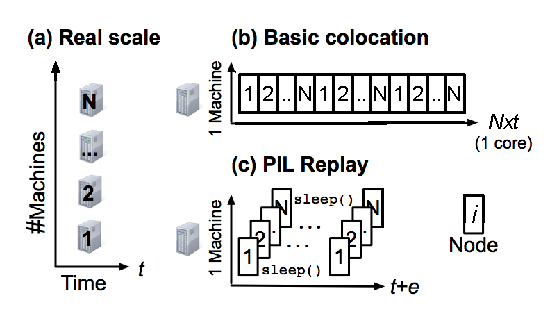
\includegraphics[height=1.75in]{F/ill/colo-hotos.eps}
%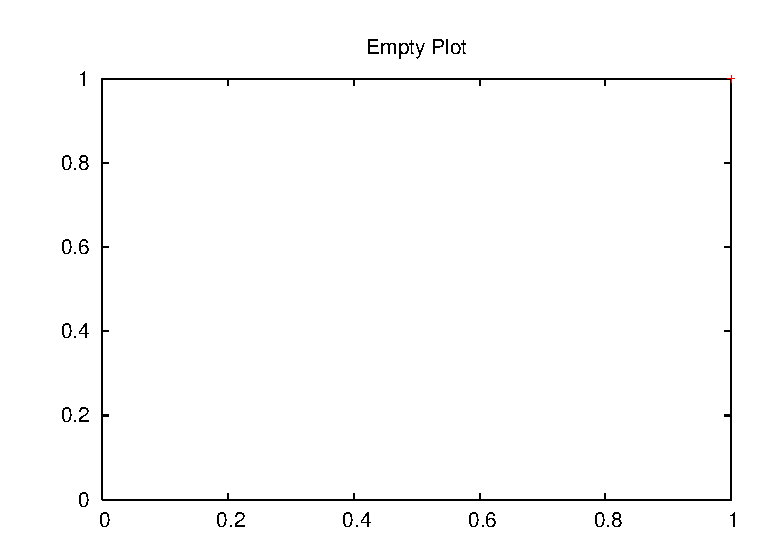
\includegraphics[height=1.75in]{F/empty.eps}
}

%\mycaption{fig-ill}{Real-scale testing, basic colocation, and scale check}{}
\mycaption{fig-ill}{Various scale-testing approaches}{The
left figure (a) illustrates a real-scale testing where the system/protocol
under test 
is deployed on $N$ machines, which illustratively takes $t$ time to complete.
%
The top figure (b) depicts a basic colocation where $N$ nodes
are packed into a single machine and exhibit CPU contention 
and context switching, which can take $N$$\times$$t$ time
to complete (in one-processor scenario).
%
The bottom figure (c) illustrates our 
processing illusion (PIL) as described in \sec\ref{sec-sck}. Here,
expensive functions are emulated with \ts{sleep()}, thus the test
time $t$$+$$e$ is similar to the real-scale testing. }


\end{figure}








\section{Scale Check}
\label{sec-sck}


We believe new methods are needed to help developers check their
systems/protocols implementation at real scale but without the hurdles of
running large test clusters.  
%
In our work, we explore a new approach to find and replay scalability bugs
in a ``cheap'' way such as on one machine, which we name {\em
  single-machine scale check} (or just ``scale check'' short).


The research question to address is: how to colocate a large number of
CPU-intensive nodes on one machine with limited resources and yet still
achieve high accuracy?
%
High accuracy implies that the colocated nodes generate a similar behavior
as if they run on independent machines.
%
The reason for inaccuracy is illustrated in Figures \ref{fig-ill}a
and \ref{fig-ill}b.
%
With real-scale testing (Figure \ref{fig-ill}a), the protocol under test
might finish in $t$ seconds.  However, with a basic colocation, the
CPU-intensive nodes contend with each other in one machine.  With only
just 1 processor core for example, the protocol under test might finish in
$N$$\times$$t$ seconds, hence the inaccuracy.
%

To address this, below we present the concept of processing
illusion (PIL) and how to find PIL-safe functions and generate output of
PIL-replaced functions.

% Figure \ref{fig-arch} depicts the major stages of our scale-check process:
% offensive function finder \textcircled{b}, memoizer \textcircled{d}, and
% replayer \textcircled{f}.



% Scalable debug time implies that the replay process can make the
% scalability bugs surface in a similar time frame ($t$$+$$\epsilon$) as in
% the real deployment ($t$), as compared in Figures \ref{fig-ill}c and
% \ref{fig-ill}a.



% Figure \ref{fig-arch} depicts the major stages of our scale-check process:
% offensive function finder \textcircled{b}, memoizer \textcircled{d}, and
% replayer \textcircled{f}.
%
% We describe each stage below in conceptual order, along with their
% technical challenges.







\def \fgw {0.85in}


\begin{figure*}[t]

\centerline{
%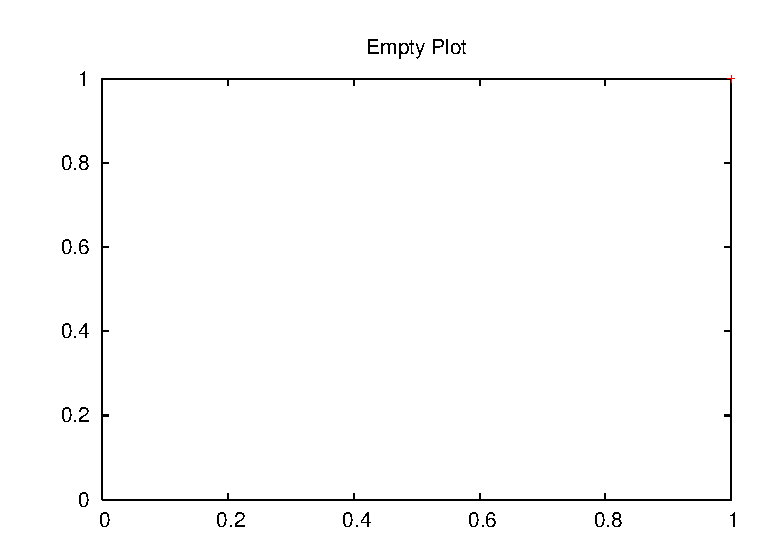
\includegraphics[height=\fgw]{F/empty.eps}
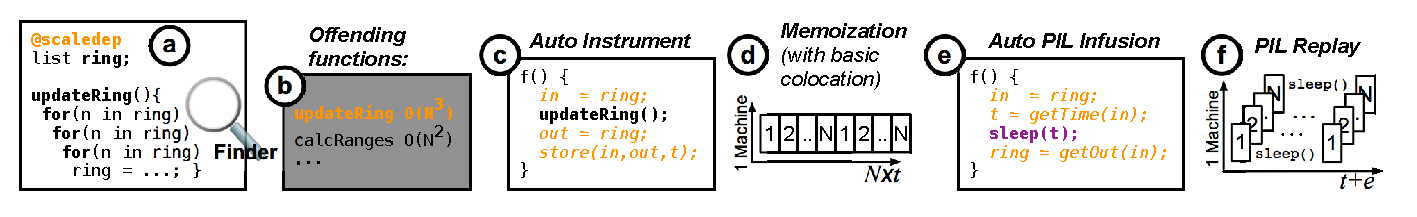
\includegraphics[height=\fgw]{F/ill/sck1-hotos.eps}
}

\mycaption{fig-arch}{The proposed flow of an automated scale-check process}{The 
figure is described in Section \sec\ref{sec-future}.}



\end{figure*}




% --------------------------------------------
\vnb\ {\bf Processing Illusion (PIL)}
%
To achieve accuracy, we must address the CPU contention delays
($N$$\times$$t$) in basic colocation (Figure \ref{fig-ill}b).
%
We propose  emulating CPU-intensive processing with {\em
  processing illusion} (PIL), which replaces an actual processing with
\sleep.
%
With PIL, an expensive function will sleep and wake up in accurate time
with the correct output.
% thus reducing contention delays and making
%replays fast (Figure~\ref{fig-ill}c).
%
As illustrated in Figure \ref{fig-ill}c, if some computations can be
emulated with \ts{sleep()} and the output data is automatically generated
given the input data, then the resulting time is more accurate ($t$$+$$e$)
to the one in real-scale testing.



PIL extends the intuition behind data-space emulation
\cite{Wang+14-Exalt}, where the insight is: ``how data is processed is not
affected by the content of the data being written, but only by its size.''
%
For PIL, our insight is that {\em ``the key to computation is not the
  intermediate results, but rather the execution time and eventual
  output.''}
%
In other words, what matters is the global cascading implication of the
long execution time of the individual nodes.


% ---------------------------------------------
\vnb {\bf Finding PIL-safe and offending functions:} One key question PIL
method raises is: which functions can be safely replaced with \sleep
\textit{without} changing the whole processing semantic?  We name them
``PIL-safe functions/code blocks.''
%
We set a rule that a PIL-safe function must have a memoizable output (\ie,
a deterministic output on a given input) and not have any side effects
such as disk I/Os, network messages, and blocking mechanisms such as
locks.  
%
Many functions satisfy the rule above, but not all PIL-safe functions
should ``take the PIL''; that is, they might not be the ``offending''
functions that lead to scalability bugs.  Thus, we raise another key
question: which functions are offending?


We learned that many offending functions contain loops that are
cluster-size dependent (\eg, a \ts{for}-loop that iterates a cluster-ring
data structure).  Some of the loops can also be a nested loop.
%
Finding such code blocks are unfortunately not straightforward.
Scale-dependent loops can span across multiple functions; in \caone,
$O(N^3)$ loops span 1000+ LOC across 9 functions.  Moreover, they can be
inside some \ts{if-else} branches reachable only from a certain
path/workload; in \caone, the last $O(N^2)$ loop is only exercised
if the cluster bootstraps from scratch.
%
All of these suggest that finding PIL-safe and offending functions require
an advanced program analysis (which we discuss later).  Such a tool will
guide the developers to decide which paths/protocols to test, to uncover
potential scalability bugs.




% -----------------------------------
\vnb {\bf Memoizing PIL-replaced functions:} PIL-safe and offending
functions will become ``PIL-replaced functions'' where their actual
processing will be skipped during replays with \ts{sleep(t)}.
%
Thus, two more questions to address are: how to produce the output if the
actual computation is skipped and how to predict the actual compute time
(\ts{t}) accurately?


The answer to the first question is {\em pre-memoization}.  That is, given
a PIL-replaced code block, we need to first execute the code block and
record the input/output around it.
%
The only way to do this on a single machine is to run the protocol with
basic colocation, which will consume some time due to the CPU contention
delays.
%
However, this will only be a {\em one-time} overhead, while the fast
PIL-infused replay stage can be repeated numerous times without
contention.



It is challenging to pre-memoize PIL-replaced functions with an offline
input-sampling method without running the protocol at least once.
%
The reason is that, in the context of large-scale, decentralized,
non-deterministic distributed systems, covering all possible input/output
pairs may require an ``infinite'' time and storage space.
%
In other words, input/output pairs depend on the precise order of message
arrivals, which can be random.
%
In a ring rebalancing algorithm for example, with $N$ nodes and $P$
partitions/node, there are $(N^{NP})^2$ input/output pairs given all
possible orderings.
%
Thus, to cap the state space, the pre-memoization stage also records
message ordering, which will be deterministically enforced during
PIL-infused replay.  With this ``order determinism,'' we do not have to
record all possible input/output pairs.  We simply record pairs that are
observed in one particular run of the protocol test.

% then the replay stage enforces order determinism.

The answer to the second question (predicting \ts{t}) is {\em in-situ time
  recording}; in addition to storing input/output pairs we also store
input/duration pairs (Figure \ref{fig-arch}c).
%
It is almost impossible to predict compute time with a
prediction/static-analysis approach.
%
As mentioned above, nested loops can span across multiple functions with
many \ts{if-else} conditions.  In a Cassandra bug, the duration of an
offending code block can range from 0.001 to 4 seconds depending on 
multi-dimensional inputs.
%
One might also wonder whether time recording is enough to hint the
developers of the potential scalability bugs (\eg, 4 seconds of compute
should raise a red flag).
%
As mentioned earlier, every implementation is unique (\sec\ref{sec-chal});
for example, in \ca{5456}, if the lock is fine-grained, the long compute
will not cause cascading impacts.
%
Furthermore, patches of scalability bugs do not always remove the
expensive computation.
%
Put simply, scalability bugs are not merely about the expensive functions,
but rather their global implications.








\section{Implementation and Integration}
\label{sec-impl}



%To make them scale-checkable on one machine, we added \locCass, \locRiak,
%and \locVold LOC respectively.




\begin{table}[t]
\begin{center}
\small
\centering
%---------------------------------
\begin{tabular}{l|r|r|r} 
{\bf } & {\bf Cassandra} & {\bf Riak} & {\bf Voldemort} \\
\hline
System               &    95757     &   18250      &  63485        \\
Unit Tests           &    18891     &   1341       &  15820        \\
\hline
(a) $+$ \sck-able        & \locCassMod  & \locRiakMod  &  \locVoldMod  \\
(b) $+$ \ts{sck} (tool)  & \locCassTool & \locRiakTool &  \locVoldTool \\
\hline
Total changes (\%)        &      5\%     &   4\%        &   2\%  
% $+$ \sck      &   \locCass  &   \locRiak   &  \locVold \\
\end{tabular}
%---------------------------------
\end{center}
\vminfive
\mycaption{tab-loc}{Integration (LOC)}{The table
quantifies our efforts in integrating \sck.
%
Riak's integration
is smaller due to the conciseness of Erlang.
%
Voldemort's integration does not include PIL for the old
bug we reproduced (more in \sec\ref{eval-colo}.)
}
\vminfive
\end{table}




We integrate our \sck methodology to three popular distributed key-value
stores: Cassandra \cite{Lakshman+09-Cassandra}, Riak \cite{RiakWeb}, and
Voldemort \cite{VoldemortWeb}.
%
The implementation of \sck involves two parts:
%
{\bf (a)} changes to make the target system ``\sck-able'' on one machine and
%
{\bf (b)} the \ts{sck} tool itself (specifically: \scass, \svold, and
\sriak).\footnote{As an analogy, part (b) is similar to specific \ts{fsck}s
  (\eg, \ts{fsck.ext3}, \ts{fsck.xfs}) while part (a) is
  similar to how file system code is modified to make \ts{fsck}
  fast \cite{Henson+06-Chunkfs, Ma+13-Ffsck}.}
% LOC
Part (a) involves
the integration of SPC, MFR, and GEDA, as well as PIL interpositioning
points.  Part (b) is the code for pre-memoization, time profiling, and
other \ts{sck} setups.
%
Table \ref{tab-loc} quantifies the integration efforts.  
%Overall, our modifications add 2-4\% of code that provide a new powerful
%functionality.
%

\vni {\bf Generality:} We show the generality of \sck with two major efforts.
First, we picked three systems and scale-checked various control-path
protocols within them, for a total of \numProt protocols:
%
\numProtCass Cassandra (bootstrap, scale-out, decommission),
%
\numProtRiak Riak (bootstrap+rebalance), and 
%
\numProtVold Voldemort (rebalancing) protocols.
%
A protocol can be built on top of other protocols (\eg, bootstrap on
gossip and failure detection protocols).


Second, we migrated \sck to a total of \numVers old and new releases:
%
\numVersCass Cassandra (v0.8.9, v1.1.10, v1.2.0, v1.2.9, v2.2.5),
%
\numVersRiak Riak (v0.14.2, v2.1.3), and
%
\numVersVold Voldemort (v0.90.1, v1.10.21).
%
This effort is also important to show how \sck can find old and new
bugs. 



\vni {\bf Simplicity:}
%
Table \ref{tab-loc} shows \sck\ requires thousands of LOC, which we
believe is a justified cost for supporting scale-checkability.  We want to
emphasize that this is a {\em one-time} cost; subsequent migrations are
fast.  Our first complete integration to Cassandra (v1.2.9) took almost a
year; we needed to learn from scratch about Cassandra and its scalability
bugs and also design \sck.  However, after \sck techniques were solid,
migration to other versions (Cassandra-v0.8.9, v1.1.10, v2.2.5) only took
{\em 1~week} each.  Next, our first integration to Riak (v0.14.2) only
took {\em 4~weeks} (although Riak was completely new to us).  A subsequent
migration (Riak-v2.1.3) only took {\em 4~days}.  The efforts for
Voldemort is also similar.
%
Overall, we expect \sck integration can be done more seamlessly with
today's DevOps practice \cite{Limoncelli+11-Devops}, where developers are
testers and testers are developers.







\if 0
All \sck techniques are straightforward to integrate.  Below are more
specific integration items we did not discuss before.
\hsg{list of all problems, existing systems are not designed
with scale checkability in mind.}
- Global lock
- Small size thread pool
- Bounded queue
\fi

\if 0
\vni {\bf Pre-Memoization:} During the pre-memoization step (with Naive
Packing), failure-detection or all timeout-related logic has to be
converted to use logical time.  This is important to remove false
positives; for example, a node might not hear any new gossip of another
node after 10 seconds, but this is due to CPU contention (thread queueing
delay) in Naive Packing.  This is a similar concern in DieCast \cite{x},
hence the time-dilation support in their VMM.  In our case, we manually
modify the application ... \hsg{how??}
\fi









\if 0
{\bf Limitations:}
\hsg{define the target protocols. the target protocol, 
the target problem, to a methodology. many P2P systems have this problem.
it cannot debug bugs that are not caused by cascading CPU problems.
There are many scalability bugs.  Just like Exalt cannot be used for our
bugs, ours cannot be used for their bugs.  At the end Sck methodology
will grow more.  So far we are limited to one machine.
The limit is the core of the one machine. To scale up we can have
more cores (co-processors with large DRAM). 
%
Also why note 10 machines? why one machine?
SCk can be extended to 10 machines, but then we need to implement
batching, because in reality each node only receives XX messages per second,
but with 50 nodes, it receives 50x messages per second.
ONe must look into this effect.
} 
\fi





\section{Evaluation}
\label{sec-sck-eval}


We now evaluate our \sck integration to Cassandra, Riak,
and Voldemort.  Our evaluation answers the following questions.
%
\sec\ref{eval-colo}: What is the maximum colocation factor achieved?
%
\sec\ref{eval-accu}: How accurate is \sck compared to real deployments?
%
\sec\ref{eval-bugs}: Can \sck find old scalability bugs?
%
\sec\ref{eval-new}: Can \sck reveal new bugs?
%
% \sec\ref{eval-mem}: How long is the output and time memoization overhead?
%
\sec\ref{eval-other}: Does our evaluation compare well with other work?


We use the Nome cluster; each machine has 16-core AMD Opteron(tm) 8454
processors with 32-GB DRAM \cite{NomeNodes}.
% link to Nome spec on website, ask Korn
%
To measure \sck accuracy (\sec\ref{eval-accu}), we compare it with real
deployments of 32, 64, 128, 256, and 512 nodes, deployed on at most 128 Nome
machines.  
%
\footnote{Our target protocols only make at most 2 busy cores per
node, which justifies why we run 8 nodes per one 16-core machine for the real
deployment. }
%



\subsection{Colocation Factor}
\label{eval-colo}

\input{fig-eval-colo}


We first show the maximum colocation factor \sck can achieve as each
feature is added {\em one at a time} on top of the other.  To recap, the
features are: processing illusion (PIL; \sec\ref{sc-pil}),
single-process cluster (SPC; \sec\ref{sc-spc}), global event driven
architecture (GEDA; \sec\ref{sc-geda}), and memory footprint reduction
(MFR; \sec\ref{sc-mem}).  The results are based on a 16-core Nome 
machine \cite{NomeNodes}.


% define maximum colocation factor
\vni {\bf Maximum colocation factor (MaxCF):} A maximum colocation factor
is reached when the target system's behavior in \sck mode starts to
deviate from the real deployment behavior.
%
Deviation happens when one or more of the following bottlenecks are
reached:
%
(1) high average CPU utilization ($>$90\%),
%
(2) memory exhaustion (nodes receive out-of-memory exceptions and crash), and
%
(3) high event ``lateness''; 
queuing delays from thread context switching can make events late to be 
processed,
although CPU utilization is not high.
%
We instrument our target systems to measure {\em event lateness} of
relevant events (\eg, gossip sending, gossip processing, and failure
detection events).  For example, if gossips should be sent every 1 second,
but they are sent every 1.5 second on average, then the lateness is 50\%.
%
We use 10\% as the maximum acceptable event lateness.
%
Note that the residual limiting bottlenecks above come from the main logic
of the target protocols, which cannot be removed with general methods.


% figures
\vni {\bf Results and observations:} Figure \ref{fig-colo} shows {\em
  different sequences of integration} to our three target systems and the
resulting maximum colocation factors.  We discuss four important findings
from this figure.

% ..
First, when multiple techniques are combined, they collectively achieve a
high colocation factor (up to 512 nodes for the three
systems respectively).
%
For example, in Figure \ref{fig-colo}a, with just adding SPC+GEDA to
Cassandra, MaxCF only reaches 136.  But with SPC+GEDA+PIL, MaxCF
significantly jumps to 512.
%
When we increase the colocation factor (+100 nodes) beyond the maximum, we
hit the residual bottlenecks mentioned before; at this point, we do not test MaxCF
with small increments (\eg, +1 node) as pre-memoization 
and profiling (step 3 in
\sec\ref{sc-summ}) takes time.
%
The bug in Voldemort's rebalancing protocol (\voldone) involve sequential
operations (no parallel CPU-intensive computations), hence GEDA and PIL
are not necessary.  
%We will add GEDA and PIL to test Voldemort's latest
%stable code which involves parallel rebalancing.



% independent
Second, distributed systems of the same type (\eg, P2P key-value stores)
are implemented in uniquely different ways.  Thus, integrations to
different systems face different sequences of bottleneck.  To show this,
we tried different {\em integration sequences}.  For example, for
reproducing \caone in Cassandra (Figure \ref{fig-colo}a), our integration
sequence is: +SPC, +GEDA, and +PIL (as we continuously hit CPU
contention).
%
For \riakone (Figure \ref{fig-colo}c), we began with MFR
as we hit a memory bottleneck first in Riak (the excessive Erlang processes;
\sec\ref{sc-mem}).
%
For \voldone (Figure \ref{fig-colo}d), we began with SPC to reduce Java VM
memory overhead in Voldemort.


Third, not all features get the chance to show their benefits as the
fundamental bottlenecks are reached.  For example, for Cassandra \caone
(Figures \ref{fig-colo}a-b), MFR is unnecessary as we will hit CPU
contention in $>$512 nodes.  For Riak \riakone (Figure \ref{fig-colo}c),
GEDA is not needed as we will hit a memory bottleneck in $>$512 nodes, and
similarly for Voldemort \voldone (Figure \ref{fig-colo}d).

% showing its full potential
Fourth, an \sck technique can hit a different bottleneck before showing
its full potential.  For example, for Cassandra, we tried two different
integration sequences (Figure \ref{fig-colo}a-b).  With 
Naive Packing\footnote{All nodes run as processes on
one machine without modification.}, we
initially hit a MaxCF of 48 nodes due to CPU contention.  At this point,
there are two choices: add SPC+GEDA (to reduce process/thread context
switching) or PIL (to reduce expensive processing).  In Figure
\ref{fig-colo}b, we tried +PIL first and we found that it does not help
much as process/thread queueing delays are still the bottleneck.
Similarly, in Figure \ref{fig-colo}a, SPC+GEDA also can only reach a
certain maximum.  This again highlights that it is the {\em combination} 
of the
techniques that make \sck powerful.


So far, \sck is limited by the single machine's resources.  To increase
colocation factor, a higher-end machine can be used.  \sck\ can also be
extended to run on multiple machines (a future work).


\subsection{Accuracy}
\label{eval-accu}

% ------- for next section
\input{def-form}
\input{fig-form}

Next, we provide a detailed accuracy evaluation of \sck.  Due to space
constraints, this section only focuses on one bug (Cassandra \caone
\cite{CA-One}, as described earlier in Figure \sec\ref{fig-mot}).  The
next section (\sec\ref{eval-bugs}) will summarize the other bugs we reproduced.


% metrics
Figure \ref{fig-form}a-d presents the  internal metrics within
Cassandra failure detection protocol that we measured for {\em every pair}
of nodes.  That is, the algorithm runs on every node A for every peer B.
%
Figures \ref{fig-accu}a-d compare in detail the accuracy of \stest without
PIL (``\ts{SCk}'') and \stestp with PIL (``\ts{SCk+PIL}'') compared to
the real deployments (``\ts{Real}'').
%
For example, $x$$=$512 implies the comparison of 512-node colocation in
\sck versus a real deployment of 512 nodes.



% ------------------------ a
Figure \ref{fig-accu}a shows the total number of flaps (alive-to-dead
transitions) observed in the whole cluster during bootstrapping.  
As described in the introduction of \sec\ref{sc-pil}, 
\stest by itself will not be accurate if all nodes are CPU intensive. 
%
However, with PIL, \sck closely mimics real deployment scenarios.  Most
importantly here, a significant \flaps does not appear until 256-node
deployment, hence techniques such as small/medium-scale testing or
mini-cluster extrapolation are not sufficient (Chapter \ref{chp-bg}).
%
Next, Figure \ref{fig-form}a defines that \flaps depends on \phi
\cite{Hayashibara+04-PhiFailureDetector}.  Every node A maintains a \phi
value for a peer node B (a total of $N$$\times$$(N$$-$$1)$ variables to
monitor).  If \phi$>$8 for B, A will declare B dead (a flap).




% ------------------------ b
Figure \ref{fig-accu}b shows the maximum \phi values observed for every
peer node; for graph clarity, from here on we only show with-PIL results.
%
For example, for the 512-node setup, the whisker plots show the
distribution of the maximum \phi values observed for each of the 512
nodes.  As shown, the larger the cluster, more \phi values exceeds the
threshold value of 8, hence the flapping.
%
Figure \ref{fig-form}b points that \phi depends on the average
inter-arrival time of when new gossips about B arrives at A (\gosAvg) and
the time since A heard the last gossip about B (\gosLast); the ``last
gossip'' is the last version number received (Figure \sec\ref{fig-mot}).
The point is that \gosLast should not be much higher than \gosAvg.



\input{fig-eval-accu}


% ------------------------ c
Figure \ref{fig-accu}c shows the whisker plots of gossip inter-arrival
times (\gosLast) that we collected for every A-B pair.  For example, for
the 512-node setup, the whisker plots represent the distribution of around
41 million gossip inter-arrival times; this large number is because a
message contains gossips of many peer nodes.  The figure shows that in
larger clusters, new gossips do not arrive as fast as in smaller clusters,
especially at high percentiles.
%
Figure \ref{fig-form}c shows that \gosLast depends on how far B's new
gossips propagate through other nodes to A (\hops) and the gossip
processing time in each hop (\gosProc).  The \hops is stable
at $log(N)$ on average in \sck and real deployment (not shown).  The
latter (\gosProc) is essentially state-update processing time (\supProc)
whenever there are state changes, which is the culprit.

% ------------------------ d
Figure \ref{fig-accu}d ({\em in log scale}) shows the whisker plots of
state-update processing time (\supProc); in the 512-node setup, we
measured around 25,000 state-update invocations.  The figure shows that at
high percentiles, \supProc is scale-dependent.  As shown in Figure
\ref{fig-form}d, \supProc complicatedly
depends on a scale-dependent 2-dimensional input (\ringTable and
\newStates); a node's \ringTable depends on how many nodes it knows,
including the partition arrangement ($\leq$$N$$\times$$P$) and \newStates
($\leq$$N$), which increases as cluster size increases.
%
%The bug was not expected because the median of \supProc is not
%scale-dependent.
%





We conclude that PIL-infused \sck mimics similar behaviors as in real
deployments and is accurate for reproducing scalability bugs.
%
As an additional note, we have applied the fix patch in both \sck (without
redoing memoization) and real deployment modes; Figure \ref{fig-accu}a
shows \flaps is always zero in both modes (``\ts{+Fix}'' lines).






\subsection{Bugs Reproduced}
\label{eval-bugs}



Table \ref{tab-bugs} lists all the \numEval bugs\footnote{Given the limited
time and number of students.}   we have reproduced (4
Cassandra, 1 Riak, and 1 Voldemort bugs).
We chose these \numEval bugs
(among the \numStudy bugs we studied) because the reports contain 
more detailed
descriptions about the bugs, the affected protocols, the affected code
version numbers, configuration setups, and the patches.  Table
\ref{tab-bugs} also shows the number of nodes needed for the bug symptoms
to surface and the quantifiable metrics of the symptoms.
%
Our first target system was Cassandra, hence the more bugs reproduced
compared to Riak and Voldemort; the latter two were added for  stronger
proof of concept.
%
Figure \ref{fig-bugs} shows the accuracy of \sck in reproducing the 6 bugs
using the metrics shown in Table \ref{tab-bugs}.
%
The first bug, \caone, has been described in \sec\ref{mot-bug} and
\sec\ref{eval-accu}.
%
We now briefly discuss the other five bugs 
(shown in Figure \ref{fig-bugs}) and then
%
make several important remarks.


Figure \ref{fig-bugs}a: In \catwo \cite{CA-Two}, 
when a node D is decommissioned from a
large cluster, all other nodes must own D's key-partitions.
This scale-dependent ``pending keyrange calculation'' is CPU intensive,
causing cluster-wide flapping, significantly observable in 256+ nodes.
The developers fixed it by caching outputs of slow methods.

Figure \ref{fig-bugs}b: \catri \cite{CA-Tri} 
is similar to the previous bug (\catwo),
but the fix was not efficient enough because in this new bug, the concept
of ``virtual nodes'' (multiple key-partitions per node) was added to
Cassandra.  The calculation is now scale-dependent to $N$$\times$$P$ and
becomes very CPU intensive.  This causes massive flapping during scaling out; 
the bug surfaced in 64+ nodes (when 32+ new nodes are added
to existing 32+ nodes). The bug was fixed with a complete 
redesign of the pending keyrange calculation.
%

\input{tab-bugs}




Figure \ref{fig-bugs}c: Interestingly, \cafour \cite{CA-Four} is 
a bug in the {\em same}
protocol as in the previous bug.  We wondered why the previous fix does
not work here.  We found that pending range calculation is now
multi-threaded; different range calculations can happen concurrently.
This new design however introduces a new coarse-grained lock that creates
a new problem;  it can block gossip processing for a long
time, thus introduce flapping (in 256+ nodes).  The fix changed the
lock management.
%
The figure also shows that, for this workload, offline time profiling
is not fully accurate as the bug is order sensitive at large scale.
We are now testing it with order determinism. 


Figure \ref{fig-bugs}d: In \voldone \cite{VOLD-One}, 
Voldemort's rebalancing was not
optimized for large clusters; it led to more stealer-donor partition
transitions as the cluster size grows (128+ nodes).  To fix this, the
developers completely changed the stealer-donor partition 
transition algorithm.


Figure \ref{fig-bugs}e: In \riakone \cite{RIAK-One}, Riak bootstrapping
employed a complex 3-stage rebalancing algorithm (claim-target,
claim-hole, full-rebalance) that each node runs to eventually converge and
achieve a  perfect balance of the ring.  Each node runs this
CPU-intensive algorithm on {\em every} bootstrap gossip received.  The
larger the cluster, the longer time perfect balance is achieved (observed in
128+ nodes).
% This decentralized
% rebalancing was fixed with a centralized rebalancing.  
For Riak, we profile the rebalancing time along with pre-memoization (with
order determinism; \sec\ref{sc-pil-3}-\ref{sc-pil-4}).  Figure
\ref{fig-bugs}f (similar to Figure \ref{fig-accu}d) compares the execution
time of the rebalance function invocations in \sck and real deployments.
The figure shows that \sck's PIL exhibits a high accuracy.


\input{fig-eval-bugs}



We make several remarks from this experience.
%
First, if \sck had existed in the first place, it might have {\em
  prevented} the Cassandra bugs; they all involve the same protocols
(gossip, rebalance, and failure detector) and create the same symptom
(high \flaps).  These bugs highlight that code evolution can introduce new
bugs in the same protocols.  In this context, \sck is highly useful.
%
Second, reproducing scalability bugs is relatively {\em easy} as we
achieve a high colocation factor.  Unlike non-deterministic bugs which
require complex timing reordering to reproduce 
\cite{Guo+11-Demeter, Leesatapornwongsa+14-Samc},
% \cite{Leesatapornwongsa+16-TaxDC},
symptoms of scalability bugs are ``deterministically scale-dependent.''
%
%
Third, different systems of the same type (\eg, key-value
store) implement similar protocols.  The {\em generality} of \sck methods
in scale-checking the protocols above can be useful to many other
distributed key-value stores.




% https://mail.google.com/mail/u/0/#inbox/1544ecd936258917






\subsection{New Bugs}
\label{eval-new}



We also scale-checked the latest stable versions of Cassandra (v2.2.5),
Riak (v2.1.3), and Voldemort (v1.10.21). 
%
In Cassandra, \sck\ shows that cluster-wide flapping resurfaces again but
only observable in 512-node deployment (\eg, decommissioning only one node
caused almost 100,000 flaps).  We submitted the bug few months back and it
is still unresolved (the fix might require new design).
%
Meanwhile, the developers suggested us to add/remove node one at a time
with 2-minute separation, which means scaling-out/down 100 nodes will take
over 3 hours; instant elasticity is not achievable.
%
%We then found out that Cassandra developers just recently started a new
%initiative and opened a new ``umbrella'' ticket (July 2016) for designing
%``Gossip 2.0'' \cite{Gossip20}, supposed to scale to
% https://issues.apache.org/jira/browse/CASSANDRA-12345
%1000+ nodes; the conversation just begun \cite{Gossip20Mail}.
% http://mail-archives.apache.org/mod_mbox/cassandra-dev/201609.mbox/%3CCAHjqPuJMkfZwp9DDX45PNBNhkoGXsPW4TFT6Zxv%2BTTz_Pg3Y%2Bg%40mail.gmail.com%3E
% maybe create a short google url ?
%
% The bug affects bootstrap, scale-out, and decommission protocols 
%
%We just submitted this new bug to the developers.  We can reproduce it in
%\sck and are currently debugging the root cause together with the
%developers.  
For Riak and Voldemort, we found that their latest-stable
bootstrap/rebalance protocols do not exhibit any scalability bug, up to
512 nodes.

\if 0
\hsg{maybe add the facts that developers suggest, 
to spread out the boot-up time. 
however, that has a challenge,
we can use Sck to find out what is a good separation,
without making the cluster not stable.}

\hsg{TODO???? the only TODO list here.}
\fi


%


\subsection{Evaluation Scope (vs. Other Work)}
\label{eval-other}

%We now compare the scale of our evaluation with Exalt's
%\cite{Wang+14-Exalt} and DieCast's \cite{Gupta+08-DieCast} in various
%dimensions:
%
\begin{enumerate}
\item {\bf Colocation factor:} DieCast is primarily evaluated with 10
nodes/machine.  Exalt runs up to 100 nodes per 16-core machine
% (limited by CPU bottlenecks).  
\sck can achieve up to \maxCF colocation factor.
However, in our view, Exalt and \sck \textit{complement each other} as
they target different types of bugs (data- vs. compute-intensive).
%
\item {\bf \#Target systems:} Exalt is integrated to two master-slave
systems (HBase and HDFS), DieCast to 3 systems (BitTorrent, RUBis, and
ISaaC), and \sck to three P2P key-value stores.
%
\item {\bf \#Target protocols:} Exalt and DieCast test write protocols and
\sck tests \numProt control-path protocols.
%
\item {\bf \#Bugs:} DieCast did not reproduce any bugs; it mainly
evaluates throughput/latency accuracy.
%
Exalt discussed 6 bugs in total (5 out of 6 are bugs in the Namenode, the
non-emulated node; \sec\ref{mot-state}).
%
\sck reproduced 6 bugs in emulated P2P nodes.
%
\item {\bf Types of bugs:} While most work focus on data-plane bugs
(\sec\ref{mot-control}, \sec\ref{mot-state}), \sck focuses on
control-plane protocols which are mainly about cluster stability (no
flapping, eventually balanced, \etc).

\end{enumerate}



\section{Conclusion}

In this chapter, we have presented our observations on scalability bugs that
highlight a need of an attention to combat them. Scalability bugs are latent
bugs that are scale-dependent that only manifest in large scale. We have also
presented our pilot work \sck, a methodology to enable developers to colocate
hundreds of nodes on one machine to emulate large-scale deployments; this helps
developers save cost of testing and speed up testing process. We have introduced
four techniques in this chapter:

\begin{enumerate}

\item {\bf Processing Illusion} (PIL) helps reduce CPU contention so
CPU-intensive nodes can be more colocated on one machine.

\item {\bf Single Process Cluster} (SPC) helps reduce memory consumption and
context switching.

\item {\bf Global Event Driven Architecture} (GEDA) helps reduce the number of
threads we need to run the systems.

\item {\bf Memory Footprint Reduction} (MFR) helps reduce memory consumption
further.

\end{enumerate}

\sck is a pilot work, it still needs a lot of manual efforts from developers to
do scale check, but we hope that this work can grab attention from system
community on combating scalability bugs.


\chapter{Related Work}
\label{chp-rel}

\chapter{Summary}
\label{chp-con}

In this proposal, we aim to unearth hidden bugs in cloud-scale distributed
systems that weaken reliability and scalability of the systems. For reliability
bugs, we focus in distributed concurrency (DC) bugs. For scalability bugs, we
focus in control-plane protocol bug, specifically in P2P storage systems.

%We started our work by performing bug studies. Based on our initial work for
%cloud bug study, we dissect DC bugs and study their critical characteristics.
%Then we look at scalability bugs that are related 

The key idea for unearthing DC bugs is advancing model checking techniques for
dmcks to tackle state-space explosion. Because existing dmcks treat every target
system as a complete \textit{black box}, and therefore perform unnecessary
reorderings of distributed events that would lead to the same explored states
(\ie, redundant executions).  To tackle the problem, we introduced
Semantic-Aware Model Checking (SAMC), a novel white-box model checking approach
that takes \textit{semantic knowledge} of how distributed events (specifically,
messages, crashes, and reboots) are processed by the target system and
incorporates that information in reduction policies. The policies are based on
sound reduction techniques such as DPOR and symmetry.

And for scalability bugs, we believe from the study that we need to scale check
distributed system implementation at real scale, not via simulation nor
extraploation. Our proposed solution is to colocate as many nodes as possible
(\eg, hundreds) on one machine without sacrificing accuracy by {\em emulate}
hardware resources such that the individual nodes behave as if they run on
independent machines. We propose four emulation concepts to mitigate hardware
contention problems. We are exploring these concepts to build scale check
methodology for checking control-plane protocols in P2P key-value stores.




% Format a LaTeX bibliography
\makebibliography

% Figures and tables, if you decide to leave them to the end
%\input{figure}
%\input{table}

\end{document}


